\documentclass{svmono}

\usepackage{type1cm}
\usepackage{makeidx}         % allows index generation
\usepackage{graphicx}        % standard LaTeX graphics tool
\usepackage{multicol}        % used for the two-column index
\usepackage[bottom]{footmisc}% places footnotes at page bottom
\usepackage{amsmath}
\usepackage{bm}
\usepackage{amssymb}
\usepackage{mathtools}
\usepackage{bbold}
\usepackage{subfigure}
\usepackage{hyperref}
\usepackage{cleveref}
\usepackage{lipsum}
\usepackage[utf8]{inputenc}
\usepackage[english]{babel}
\usepackage{pdfpages}
\usepackage[top=3cm,bottom=4cm,outer=3.5cm,inner=3.5cm]{geometry}
\usepackage[normalem]{ulem}
\usepackage{braket}
\usepackage{tikz}
\usepackage{ifthen}
\usepackage{dsfont}
\usetikzlibrary{tikzmark}

\newcommand{\todo}[1]{{\color{cyan} \scshape !!! #1 !!!}}

%!TEX root = thesis.tex
%%%%%%%%%%%%%%%%%%%%%
\def\ri{\mathrm i}
\def\re{\mathrm e}
\def\rd{\mathrm d}
\def\rD{\mathcal D}
\def\hc{{\rm h.c.}}
\def\tr{{\rm tr}}
\def\C{\mathcal{C}}
\def\DC{\Delta\C}
\def\GX{\Gamma X}
\def\DCav{\overline{\Delta\C}}
\def\up{\uparrow}
\def\down{\downarrow}
\def\pdag{{\vphantom\dag}}
\def\pp{\vphantom{n'}}
\def\Cav{\overline\C}
\def\MH{H}
\def\HS{\mathcal{H}}
\def\FS{\mathcal{F}}
\def\omegaT{\tilde{\omega}}
\def\tbc{{\\[1cm]\bf \color{red}[TO BE CONTINUED...]}}
\newcommand{\ave}[1]{\langle #1 \rangle}
\newcommand{\sign}[1]{\text{sign}\left( #1 \right)}
\newcommand{\commutator}[1]{\left[ #1 \right]}
\newcommand{\anticommutator}[1]{\left\{ #1 \right\}}
\newcommand{\brlr}[1]{\left( #1 \right)}
\newcommand{\abs}[1]{\left| #1 \right|}


\makeindex % used for the subject index
%%%%%%%%%%%%%%%%%%%%%%%%%%%%%%%%%%%%%%%%%%%%%%%%%%%%%%%%%%%%%%%%%%%%%%%%%%%%%%%%

\begin{document}

\author{Andreas Haller}
\title{On the tuning of particle transport,\\ the fabrication and the detection of\\ topological phases of matter}
\subtitle{PhD Thesis}

\maketitle

\frontmatter%%%%%%%%%%%%%%%%%%%%%%%%%%%%%%%%%%%%%%%%%%%%%%%%%%%%%%%%%%%%%%%%%%%%

%!TEX root = thesis.tex
%%%%%%%%%%%%%%%%%%%%%

\begin{dedication}
    Let's call it a PhD {\tiny (please)}
\end{dedication}

%!TEX root = thesis.tex
%%%%%%%%%%%%%%%%%%%%%
\chapter*{Acknowledgments}
\addcontentsline{toc}{chapter}{Acknowledgments}
Now that I am right at the finish line, besides being happy that the exhaustive part is finally over, I feel a great deal of gratitude.
I would simply not have made it through, were it not for the wonderful people that take part in my life.

First of all I want to thank the members of the examination board for taking the time to evaluate the dissertation.
I know that you are all incredibly busy, and truly appreciate your tremendous effort in training the next generation of scientists.

I want to express my deep gratitude towards {\it Prof. Michele Burrello}.
You are one of the first persons I approach for professional advice, and I am always astonished by how much you know about physics.
Thank you so much for your mentoring, and for inviting me to the Niels Bohr Institute.
Brainstorming with smart and inspiring people is one of the best experiences during my PhD.
One of the best examples out of of this ``equivalence class'' of individuals is {\it Prof. Pietro Massignan}.
I am looking forward to visiting the post-pandemic Primavera Sound Festival with you and Hélia.
Most of my academic collaborators are Italian, and although I am not a fan of cliches, I must admit that they are indeed very passionate:
Thank you, {\it Michele Filippone}, for your regular motivation speeches during the time we worked together, for having me around in Geneva, for showing me the Bains des Pâquis and warning me about drinking cold water after a Swiss Fondue.
Speaking of passionate Italians, I want to express my gratitude towards {\it Jun.-Prof. Jamir Marino}.
Thank you ``für den frischen Wind'' as we Germans like to say, for your feedback regarding my thesis and for putting so much effort in a lively scientific exchange, which is incredibly hard to maintain right now.
By now it is clear to me that an academic career is unavoidably linked to a level of uncertainty: be it compensation, doubting yourself or feeling unrecognized and irrelevant, it results in a lot of unnecessary distraction from actual work.
I am grateful to the head of our group, {\it Prof. Peter van Dongen}, who managed to eliminate most of these uncertainties during the period of my PhD.
Thank you for your scientific advice, for being part of the examination board, and for carefully reading this thesis.
I am glad that you consider me part of your little ``bubble'', and I wish you the best for the future.
I want to thank {\it Prof. Patrick Windpassinger} for writing a letter of recommendation to the graduate school and for being part of the examination board.
My PhD would have been impossible without the scholarship of the Graduate School Materials Science in Mainz (MAINZ) and the Max Planck Graduate Center (MPGC).
Special thanks to {\it Michael Fuchs}, {\it Katrin Klauer}, and to {\it Prof. Thomas Speck}.

My student's life would have been pretty sad and lonely without a group of fellows: {\it Matteo Campo}, {\it Álvaro Díaz Fernández}, {\it Achim Harzheim}, {\it William Janke}, {\it Johannes Jünemann}, {\it Philipp Schmoll} and {\it Niklas Tausendpfund}.
Thank you for taking the journey with me and for reading part of this thesis.
I already miss our discussions, joint conferences, lunches and coffee breaks.

Music is a big part of my life, and it hurts me very much that these past few months were exceptionally quiet.
To all my musician friends, in particular to {\it Simon Engelhardt}, {\it Carlos Wagner} and the Grundfunk family:
There will be a time when we enjoy once more the incredible joy of playing with real people, at a real stage, and in front of an audience.
Until then, hold on tight and keep on practicing.

Sometimes (mostly Tuesdays) I came in late due to the merciless morning squash matches between me and {\it Andreas Dittinger}, {\it Fabian Kolf} and {\it Maximilian Shaikh-Yousef}.
Before my passion for squash, I was happily climbing like an ape during my free evenings in the Blockwerk Mainz with {\it Johannes} and {\it Julia Hofmann}, {\it Ruben Hoffmann} and the ``BFE crew'', which again resulted in me coming in late to university.
At other times, I overslept because of a merry wine-drinking session with our favorite upstairs neighbors {\it Laura Hollegger} and {\it Max Henderson}.
To all of my dear friends: Thanks for the joy and happiness you bring into my life.

Family always comes first, although by now we live a bit detached from each other.
I want to thank my brother-in-law, {\it Stefan Stamer}, and my parents-in-law, {\it Helma Heinz-Stamer} and {\it Thomas Stamer}.
You know me for half of my life now, and I can only imagine how annoying it must have been for you to meet me while I was a long-haired teenager.
Joking aside, I always feel warm and welcome when I am around you, and I thank you deeply for trusting me with the biggest treasure you have:
{\it Susanne}, you are the love of my life.
I don't know if you remember our chat nine years ago, but you are the reason why I pursued a career as a Physicist, which, besides marrying you, was one of the best decisions of my life.
I want to thank my grandma, {\it Irmgard Heinz}, and I hope this message reaches you somehow.
You were the sweetest person of age that I know, always happy when we passed by, and never showed your disappointed if we were busy otherwise.
I remember our joint trip to the canary islands with Susanne like it was yesterday, because it woke my curiosity to travel the world.

To my siblings, {\it Michael Haller} and {\it Astrid Fengler}.
Thank you for your patience with me.
% I've not always been the best little brother, and certainly was a rascal when I was younger.
Despite all our differences, I know that I can always count on you, and I am deeply grateful for having you in my life.
% Since my parents do not understand english, but certainly deserve one of the biggest thanks, allow me to switch languages for a while.
{\it Liebe Mama, lieber Papa}, ihr habt mein Studium stets unterstützt, auch wenn ihr keinen Bezug zu dem Thema habt.
Euch war es stets das oberste Gut, dass wir die wichtigen Entscheidungen unseres Lebens unvoreingenommen und selbstständig getroffen haben.
Nur durch dieses große Vertrauen in uns sind wir zu den Personen geworden, die wir heute sind.
Dafür liebe ich euch und bin euch unendlich dankbar.

Al mio capo {\it Prof. Matteo Rizzi}:
You made all of this possible by shaping me into the scientist I am today.
I remember very well when I entered your office for the first time, not knowing what to expect, a little shy and intimidated by your wisdom.
Although I knew so little at the time we started working together, you never lost interest and aided me to the best of your abilities.
I could not have been guided better and I am proud to call myself your student.
With all of my heart, I deeply thank you for our joint time and wish the best to you, Michela, and Giovanni.

I am grateful to everyone that shaped and decorated the path of my PhD.
It has been a wonderful experience, and I would do it all over again.


\tableofcontents

%!TEX root = thesis.tex
%%%%%%%%%%%%%%%%%%%%%
\extrachap{Acronyms}
\begin{description}[PUTLONGEST]
    \item[ABC]{Spelled-out abbreviation and definition}
    \item[BABI]{Spelled-out abbreviation and definition}
    \item[CABR]{Spelled-out abbreviation and definition}
\end{description}

\extrachap{Definitions}
\begin{description}[PUTLONGEST]
    \item[$\MH$]{Full Hamiltonian (with interactions)}
    \item[$\MH_0$]{Kinetic Hamiltonian (tight-binding part)}
\end{description}



\mainmatter%%%%%%%%%%%%%%%%%%%%%%%%%%%%%%%%%%%%%%%%%%%%%%%%%%%%%%%%%%%%%%%%%%%%%

%%%%%%%%%%%%%%%%%%%%%%%%%%%%%%
%!TEX root = thesis.tex
%!TeX spellcheck = en-US,en-DE
%%%%%%%%%%%%%%%%%%%%%%%%%%%%%%
%
\chapter*{Introduction}
\addcontentsline{toc}{chapter}{Introduction}
%
In this thesis, we investigate the effects of interactions on several different quasi one-dimensional ladder models of fermions and bosons.
Our models are motivated from the ``building blocks'' of state-of-the-art experiments such as those employed in the framework of ultracold atoms trapped in optical lattices: complex tunneling amplitudes, diagonal cross hoppings and tunable (repulsive/attractive) interactions.

Taken the customary terminology for granted, let me start by a brief summary of the new results we established during the period of this thesis, presented in \cref{part:results}.
The analytical and numerical methods employed in our works build up on the theoretical concepts illustrated in \cref{part:theory}.

In fermionic systems, we found a possibility to flexibly tune the zero frequency component of the conductivity at zero temperature (a.k.a. the Drude weight) by repulsive density-density interactions (see \cref{drude_increased1}).
The enhancement of this quantity under repulsive interactions is contradicting the ``common wisdom'' for one-dimensional quantum which should always show a decreasing Drude weight.
The ``loophole'' is given through the slim 2D extension of our ladder, which allows to generate pseudospin polarized band structures which, ultimately, lead to the mentioned effects on the Drude weight.
Our results are therefore interesting for the modification of transport properties of coupled-wire systems in general.
The analytic concepts necessary to comprehend this paper are illustrated in \cref{sec:periodic_potentials,sec:tight_binding_systems,sec:tomonaga_LL,sec:LL_with_spin}.
In addition, we use matrix product state (MPS) simulations, which are presented in \cref{ch:matrix_product_states}.

We study the emergence of so-called helical liquids by repulsive interactions (see \cref{one_half1,integer1}) and density-assisted hoppings (see \cref{chiral1}).
In general, such phases result from a commensurability between particle density and flux, and share many similarities to the phases encountered in the Quantum Hall effect.
In this sense, some of the quasi one-dimensional helical phases can be interpreted as the predecessor of topological order, thus sometimes dubbed pre-topological, if they have a natural extension to 2D.
For fermions (see \cref{one_half1}), we study the emergence of an exotic phase located at particle filling factor $\nu=1/2$ which naturally extends to a fractional Quantum Hall phase, i.e. the bosonic $K=8$ state.
We then also study a similar phase in a ladder of hard-core bosons (see \cref{integer1}), located at filling factor $\nu=1$.
In both cases, we derive the phase diagram through renormalization group (RG) theory calculations and test our hypotheses through MPS simulations.
The introduction to the path integral formalism and RG is found in \cref{sec:properties_of_real_scalar_fields_and_their_correlations,sec:renormalization_group_theory}.

A natural quest in the context of topological insulators concerns the measurement of the topological invariant, especially in the case of interacting systems, where a priori it does not amount to a band dispersion quantity.
For chiral symmetric systems, we propose a simple dynamical protocol based on the mean chiral displacement which provides a tomography of the topological index (see \cref{mcd1}).
We furthermore provide a basic experimental blueprint in order to implement our proposition.
On the analytic side, we rely on standard band theory and test our hypotheses with MPS simulations.
The introduction to topological phases of matter in general is found in \cref{ch:topological_phases_of_matter}.

As an undergraduate student studying elementary physics, I always thought of quantum particles as plane waves living in the differential-geometric world of ``first quan\-ti\-zation'' which (at least for me) was both beautiful and frustrating at the same time as the task of solving the most simple problems may become quite involved, if not even impossible.
The modern approach is not a straightforward attempt to solve the real-space wave function by integrating a given Schrödinger equation: It rather sticks to an alternative representation in the algebraic world of ``second quantization'' where the action of operators dictates all physical consequences.
I must admit that I find the nomenclature of ``first'' and ``second'' somewhat confusing, as there is no such thing as two consecutive ways of quantization -- it's just two alternative and consistent ways of describing the same theory.
Ultimately, I've learned to accept this issue as a result of chronology: the original formulation of quantum mechanics is commonly called first quantization, in which the (motion of the) particle is quantized and possible electromagnetic fields or potentials are considered classical, whereas quantized fields have been formulated in the language of second quantization.
However, as we will see soon, the advantage of second quantization manifests itself in a simpler and more efficient way to describe many-body systems such that its development can be seen as the first major cornerstone in the emergence of quantum field theory.

Independent of the formulation, be it first or second, all quantum theories require certain basic concepts:
all quantum states are represented by state vectors $\{|q\rangle\}$ forming a complete basis of the Hilbert space and observables are defined through Hermitian operators acting on that space.
The states are given through a set of good quantum numbers $q$, e.g. for the electron of hydrogen $(n,l,m)$ associated with the total energy, angular momentum and its projection along the primary axis.

In \cref{part:theory}, I review these concepts in more detail.
The first sections, i.e. \cref{sec:creation_and_annihilation_operators,sec:representation_of_generic_operators,sec:periodic_potentials,sec:tight_binding_systems}, are aimed to guide undergraduate students which are new in the field of condensed matter.
To become familar with the basics, I review the tight binding approximation in \cref{sec:tight_binding_systems}, derived from the Kronig-Penney model in the strong potential limit (see \cref{sec:periodic_potentials}).
I then illustrate the treatment of interactions on top of a quadratic/non-interacting Hamiltonian which is a crucial tool in the understanding of quantum matter.
This becomes particularly easy in the concept of Luttinger liquids (see \cref{sec:tomonaga_LL}) as a first example of a quantum field theory satisfying the algebra of a quantum harmonic oscillator.
The key in Luttinger liquids is that the effective theory describing intrinsically interacting microscopic models remains quadratic at the operator level, and as such effectively non-interacting.
I then use the formalism of path integrals (see \cref{sec:properties_of_real_scalar_fields_and_their_correlations}) to derive analytic expressions of the correlation functions.
A common interaction which potentially melts the Luttinger liquid phase is a sine-Gordon term, which I derive in \cref{sec:LL_with_spin}.
In order to treat such higher-order interactions analytically, I introduce the concept of renormalization group theory (see \cref{sec:renormalization_group_theory}), which provides a platform to study if and when the Luttinger liquid basis must be exchanged in favor of the collective many-body basis dictated by the interactions.
One major drawback is that renormalization group theory relies on many simplifications along the way to make the calculation amendable, and microscopic details of the model are often lost in the approximations.
These details are exchanged in favor of ``universality'', an effective theory which describes the physical properties of a family of different microscopic models at long scales.
In this framework, it is thus not intended to provide quantitative predictions for the microscopic theories, such that numerical tools become essential.

A brute force calculation of a full solution scales exponentially with the number of constituents, such that exact diagonalization of interacting models is limited to small system sizes (e.g. $\sim 20$ sites for interacting spin-1/2 models in typical studies).
This stresses the need for more efficient numerical techniques in the study of non-perturbative regimes which cannot be amended analytically.
In this thesis, I mainly use matrix product states (MPS), and I illustrate the main concepts in \cref{ch:matrix_product_states}.
In \cref{sec:tensor_networks,sec:reduced_density_matrix_and_renyi_entropy}, I begin with a general introduction into the field of tensor networks and MPS.
A general discussion of scaling relations of the entanglement entropy is used to explain the effectivity of the MPS Ansatz (see \cref{sec:scaling_relations_of_the_entanglement_entropy}).
As a natural extension to MPS, I then introduce matrix product operators (MPO) in \cref{sec:matrix_product_operators} which are most useful to express the Hamiltonian, and to calculate observables in general.
After the preliminary introductions, I introduce the basic strategy to approximate ground states based on an MPS Ansatz in \cref{sec:variational_ground_state_search}.
This algorithm is quite similar to the (imaginary) time evolution presented in \cref{sec:time_evolution}, which can also be used to simulate finite temperature systems, presented in \cref{sec:finite_temperature}.
I conclude the chapter by a basic introduction into symmetry invariant MPS formulations, discussed in \cref{sec:exploiting_symmetries}.

Perhaps the most interesting behavior of quantum many-body physics is that of so-called emergent phenomena -- e.g. the appearance of quasi-particles which extend the canonical statistical properties of fermions and bosons in low dimensions, or the presence of robust quasi-particles at the boundaries of a topological insulator.
For a basic overview of this topic, I review the classification of non-interacting topological matter in \cref{ch:topological_phases_of_matter}.
The key concept for the full classification is based on topological band theory, presented in \cref{sec:topological_band_theory}, a genuinely non-interacting formulation of symmetry protected topological phases of matter.
The notion of the topological index arises from the Berry phase and the Berry connection, and I recap the original paper.
As an example, the Su-Schrieffer-Heeger chain is then explored in \cref{sec:the_SSH_chain} to apply the introduced concepts.
I conclude the third chapter by explaining the classification of topological insulators and superconductors in \cref{sec:Periodic_table_of_topological_insulators_and_superconductors}.

In \cref{part:results}, I summarize my original contributions to our published works, which are then presented in a thematic manner.
This thesis is concluded by a summary and perspectives about interesting future directions.


%!TEX root = thesis.tex
%%%%%%%%%%%%%%%%%%%%%

\begin{partbacktext}
    \part{Theoretical Prerequisites}
    \label{part:theory}
\end{partbacktext}

%!TEX root = thesis.tex
%%%%%%%%%%%%%%%%%%%%%
%%%%%%%%%%%%%%%%%%%%%%%%%%%%%%%%%%%%%%%%%%%%%%%%%%
%%%%%%%%%%%%%%%%%%%%%%%%%%%%%%%%%%%%%%%%%%%%%%%%%%
\chapter{The quantization of motion and fields}
\label{ch:the_quantization_of_motion_and_fields}
%%%%%%%%%%%%%%%%%%%%%%%%%%%%%%%%%%%%%%%%%%%%%%%%%%
%%%%%%%%%%%%%%%%%%%%%%%%%%%%%%%%%%%%%%%%%%%%%%%%%%
%
%
% In the introductory sections I am being pragmatic on purpose, in a sense of trading mathematical rigor with a comprehensive introduction in the theory concepts to safely guide the reader through the computations performed later in this thesis.\\
As an undergraduate student studying elementary physics, I always thought of quantum particles as plain waves living in the differential-geometric world of ``first quan\-ti\-zation'' which (at least for me) is both beautiful and frustrating at the same time as the task of solving the most simple problems may become quite involved, if not even impossible.
The modern approach is not a straightforward attempt to solve the real-space wave function by integrating a given Schrödinger equation, it rather sticks to an alternative representation in the algebraic world of ``second quantization'' where the action of operators dictate all physical consequences.
I must admit that I find the nomenclature of ``first'' and ``second'' somewhat confusing, as there is no such thing as two consecutive ways of quantization -- it's just two alternative and consistent ways of describing the same theory.
Ultimately, I've learned to accept this issue as a result of chronology: the original formulation of quantum mechanics is commonly called first quantization, in which the (motion of the) particle is quantized and possible electromagnetic fields or potentials are considered classical, wheres quantized fields have been formulated in the language of second quantization.
However, as we will see soon, the advantage of second quantization manifests itself in a simpler and more efficient way to describe many-body systems such that its development can be seen as the first major cornerstone in the development of quantum field theory.
\\

Regardless on the formulation, be it first or second, all quantum theories require certain basic concepts:
all quantum states are represented by state vectors $\{|q\rangle\}$ forming a complete basis of the Hilbert space and observables are defined through Hermitian operators acting on that space.
The states are given through a set of good quantum numbers $q$, e.g. $(n,l,m)$ associated to the total energy, angular momentum and its projection along the primary axis for the electron of hydrogen.
The first section ``On the quantization of motion and fields'' reviews these basic concepts in more detail and outlines the solution of atoms trapped in a harmonic potential in both differential and algebraic formulation.
I will also illustrate the treatment of small perturbations on top of a quadratic/non-interacting Hamiltonian which is a crucial tool in the understanding of quantum matter.
The importance of these solutions becomes clear after I introduce Luttinger liquids as first example of a quantum field theory satisfying the algebra of a quantum harmonic oscillator.
\\

Ultimately, there is few detailed things to say analytically about truly many-body phases of matter as the complexity of finding a full solution scales exponentially with the number of constituents.
This stresses the need of numerical techniques in the study of non-perturbative regimes which cannot be amended analytically.
In this thesis, I mainly use matrix product states, which is why I provide a section here which highlights the basic ideas and outlines benefits and shortcomings compared to other techniques.

Perhaps the most interesting behavior of quantum many-body physics is that of so-called emergent phenomena -- e.g. the appearance of quasi-particles which extend the canonical statistical properties of fermions and bosons in low dimensions, or the presence of robust quasi-particles at the boundaries of a topological insulator.
In order to perceive a basic overview in this topic, I conclude the introduction with a review on the classification of non-interacting topological matter and finish with some general statements on interacting topological insulators.
\\

The present chapter is inspired by a number of excellent books and lectures such as~\cite{AshcroftMermin1978,AltlandSimons2010,BruusFlensberg2004,Czycholl2016,FetterWalecka2003,Giamarchi2003} extending the basic aspects of quantum mechanics to a modern way of understanding quantum field theory in general.

%%%%%%%%%%%%%%%%%%%%%%%%%%%%%%%%%%%%%%%%%%%%%%%%
\section{Creation and annihilation operators}
\label{sec:creation_and_annihilation_operators}
%%%%%%%%%%%%%%%%%%%%%%%%%%%%%%%%%%%%%%%%%%%%%%%%
Consider a complete set of quantum numbers $\{\alpha\}$ which label a normalized set of states $\{\ket{\alpha}\}$ spanning the full Hilbert space $\HS^1$ of a generic single particle system described by the (time-independent) Schrödinger equation
\begin{align}
    \MH \ket{\alpha} = \varepsilon_\alpha\ket{\alpha}.
\end{align}
The single particle wave function $\Psi_\alpha(r)$ of a quantum state occupying $\alpha$ is defined as the inner product of the vector $\ket{\alpha}$ with the real-space covector $\bra{r}\in\HS^*$, i.e.
\begin{align}
    \Psi_\alpha(r) \coloneqq \braket{r|\alpha}.
\end{align}
It is is thus understood as the coefficients for the basis transform $\ket{\alpha}\rightarrow\ket{r}$, i.e.
\begin{align}
    \ket{\alpha} = \int{\rm d}{r}\, \Psi_\alpha(r) \ket{r}.
\end{align}
According to the basic postulate of quantum mechanics, the two-particle wave function with quantum numbers $\alpha_1$ and $\alpha_2$ is given by the (anti-) symmetrized product
\begin{align}
    \Psi_{\alpha_1,\alpha_2,\nu}(r_1,r_2) = \frac1{\sqrt2}\left(\braket{r_1|\alpha_1}\braket{r_2|\alpha_2} + \nu\braket{r_2|\alpha_1}\braket{r_1|\alpha_2}\right),
\end{align}
depending on the particle statistics upon exchange of their position, i.e. $\nu=\pm1$ for bosons and fermions, respectively.
The two-particle wave function can thus be represented by a more simple inner product
\begin{align}
    \Psi_{\alpha_1,\alpha_2,\nu}(r_1,r_2) = \left(\bra{r_1}\otimes\bra{r_2}\right)\ket{\alpha_1 \alpha_2}_\nu
\end{align}
which is given by the symmetric Kronecker product
\begin{align}
    \ket{\alpha_1 \alpha_2}_\nu = \frac1{\sqrt2}\left(\ket{\alpha_1}\otimes\ket{\alpha_2} + \nu\ket{\alpha_2}\otimes\ket{\alpha_1}\right).
\end{align}
In general, the symmetric $N$-particle state vector is an element of the $N$-particle Hilbert space $\HS^N = \bigotimes_{i=1}^N\HS$ and reads
\begin{align}
    \ket{\alpha_1,\alpha_2,\dots,\alpha_N}_\nu = \frac1{\sqrt{N!\prod_{\alpha}(n_\alpha!)}}\sum_P \nu^{1-\sign{P}/2}\ket{\alpha_{P(1)}}\otimes\ket{\alpha_{P(2)}}\otimes\dots\otimes\ket{\alpha_{P(N)}}.
    \label{eq:symmetric_many_body_state}
\end{align}
In the above equation, we assume ordered quantum numbers (e.g. increasing positions along a wire, or increasing energies), denote the total number of particles with quantum number $\alpha$ as $n_\alpha$ and $\sign{P}$ the sign of the permutation $P\in S^N$ of the permutation group [$\sign{P}=\pm1$ if the permutation is even/odd].
\\

The representation in the ordered expression of \cref{eq:symmetric_many_body_state} is not particularly compact since equal values of $\alpha$ may appear $n_\alpha$ times in the $N$-letter long ket -- the occupation number representation removes this redundancy.
The states in this representation are then given by
\begin{align}
    \ket{n_1, n_2, \dots}_\nu = \ket{\underbrace{\alpha_1,\alpha_1,\dots,\alpha_1}_{n_1}, \underbrace{\alpha_2, \alpha_2,\dots, \alpha_2}_{n_2}, \alpha_3, \dots}
\end{align}
and they span the space $\FS^N$ of the symmetrized $N$-particle states $\sum_{i} n_i = N$.
Thus, the subset $\FS^N\subset \HS^N$ contains all $N$-particle states which transform according to the basic postulate of quantum mechanics such that any physical state $\ket{\Psi}\in\HS^N$ can be written as a linear superposition of the Fock states
\begin{align}
    \ket{\Psi}_\nu = \sum_{\sum_i n_i = N}c_{n_1,n_2,\dots}\ket{n_1,n_2,\dots}_\nu.
\end{align}
The full Fock space $\FS$ is defined as a direct sum of all vector spaces with fixed quantum number $N$, i.e.
\begin{align}
    \FS = \bigoplus_{N=0}^\infty \FS^N
\end{align}
including the one-dimensional vacuum space commonly denoted by $\{\ket{0}\}=\FS^0$.
\\

Let us now impose a linear map $a^\dag_i:\FS\rightarrow\FS$ connecting the individual subsets through
\begin{align}
    a^\dag_i\ket{n_1,\dots,n_i,\dots}_\nu = \sqrt{n_i+1}\nu^{\sum_{j<i}n_j}\ket{n_1,\dots,n_i+1,\dots}_\nu
    \label{eq:creation}
\end{align}
in which fermionic states must be understood ${\rm mod}_2$ such that the Pauli exclusion principle is explicitly satisfied: $a^\dag{}^2\ket{0}=a^\dag\ket{1}={\rm mod}_2(1+1)\ket{{\rm mod}_2(1+1)} = 0\ket{0} = 0$.
Notice that through the linear map we can express the canonical basis of any subset $\FS^N\subset\FS$ as
\begin{align}
    \ket{n_1,n_2,\dots}_\nu = \prod_i\frac1{\sqrt{n_i!}}\left(a^\dag_i\right)^{n_i}\ket{0}_\nu,
    \label{eq:Fock_basis}
\end{align}
and as such have a tool which promotes the vacuum to any state of the full Fock space.
\begin{figure}
    \centering
    \subfigure[]{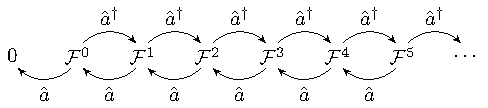
\includegraphics{figures/connected_fock_space_bosons.pdf}}
    \hfil
    \subfigure[]{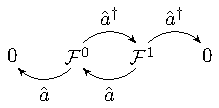
\includegraphics{figures/connected_fock_space_fermions.pdf}}
    \caption{(a) Subspaces $\FS^N$ of $N$-particle bosonic states $\ket{N}$ characterized by a single quantum number. Adjacent spaces are connected through the linear maps $a^{(\dag)}$ defined in \cref{eq:creation,eq:annihilation}. (b) Subspaces for a fermionic system characterized by a single quantum number.}
    \label{fig:my_label}
\end{figure}
Notice the absence of the phase $\nu$ on the right hand side which is due to the fact that the product is ordered.
For this reason, the linear maps $a^\dag_i$ are commonly called creation operators which is what we will call them in the remaining part of this thesis.
Two different linear maps $j<i$ satisfy the following equation
\begin{align}
    a^\dag_i a^\dag_j\ket{n_1,n_2,\dots}_\nu = \nu a^\dag_ja^\dag_i\ket{n_1,n_2,\dots}_\nu,
\end{align}
and thus span the famous (anti-) commutation relation
\begin{align}
    \commutator{a^\dag_i, a^\dag_j}_\nu \coloneqq a^\dag_i a^\dag_j - \nu a^\dag_j a^\dag_i = 0.
\end{align}
From the Hermitian adjoint of the equations before we get the condition
\begin{align}
   \braket{n_1,\dots,n_i,\dots | a^\pdag_i | m_1, \dots, m_i,\dots}_\nu =
   \sqrt{n_i+1}\nu^{\sum_{j<i}n_j} \delta_{n_1,m_1}\dots\delta_{n_i+1,m_i}\dots
\end{align}
and thus
\begin{align}
   a^\pdag_i \ket{n_1, \dots, n_i,\dots}_\nu =
   \sqrt{n_i}\nu^{\sum_{j<i}n_j} \ket{n_1, \dots, n_i-1,\dots}_\nu,
   \label{eq:annihilation}
\end{align}
from which we obtain the algebra relations of the creation/annihilation operators
\begin{align}
    \commutator{a^\pdag_i,a^\dag_j}_\nu = \delta_{i,j},
    \quad
    \commutator{a^\pdag_i,a^\pdag_j}_\nu = 0,
    \quad
    \commutator{a^\dag_i,a^\dag_j}_\nu = 0.
    \label{eq:Heisenberg_algebra}
\end{align}
Proceeding in a reversed manner,~\cref{eq:Fock_basis} is a consequence of the Stone-von Neumann theorem which states that, given the Heisenberg algebra defined through~\cref{eq:Heisenberg_algebra}, the action of the operators and the representation of the Fock basis is unique (up to unitary transformations)~\cite{Hall2013}.

To conclude this first section, a change of basis $\{\ket\alpha\}\rightarrow\{\ket\beta\}$ yields\footnote{Remember that $\mathbb1 = \sum_\alpha\ket{\alpha}\bra{\alpha}$, $\ket{\beta} = \sum_\alpha\ket{\alpha}\braket{\alpha|\beta}$ and $\ket{\beta}=a^\dag_\beta\ket{0}$, leading to \cref{eq:creation_annihilation_basis_rotation}.} a unitary transformation of the operators
\begin{align}
    a^\dag_\beta = \sum_\alpha \braket{\alpha|\beta}a^\dag_\alpha,
    \quad
    a^\pdag_\beta = \sum_\alpha \braket{\beta|\alpha}a^\pdag_\alpha
    \label{eq:creation_annihilation_basis_rotation}
\end{align}
which requires only a computation of the single-particle matrix elements $\braket{\alpha|\beta}$.
Before we move on to the representation of observables, a word on common notations: Quite often the authors assume a certain particle statistics and operator algebra at the beginning of their work which implies a constant (and thus dropped) subscript $\nu$.
In such cases, fermionic annihilation operators are mostly identified through the letter $c$ whereas $b$ often corresponds to bosonic operators.
Furthermore, a common convention identifies the commutator through crotchets
\begin{align}
    \left[\hat A,\hat B\right]\coloneqq\commutator{\hat A,\hat B}_+ = \hat A\hat B - \hat B\hat A
\end{align}
and the anticommutator through curly braces
\begin{align}
    \anticommutator{\hat A,\hat B}\coloneqq\commutator{\hat A,\hat B}_- = \hat A\hat B + \hat B\hat A.
\end{align}
Let me also provide a useful expression to evaluate the commutation relation of operator products recursively
\begin{align}
    \commutator{\hat A, \hat B \hat C}_\pm
    &= \hat A\hat B\hat C \mp \hat B\hat C\hat A + \hat B\hat A\hat C - \hat B\hat A\hat C
    \\
    &= \commutator{\hat A, \hat B}_\pm\hat C \mp \hat B\hat C\hat A \mp \hat B\hat A\hat C
    = \commutator{\hat A, \hat B}_\pm\hat C \mp \hat B\commutator{\hat A,\hat C}.
    \label{eq:recursive_commutation}
\end{align}
In many cases, the sets of quantum numbers are continuous (e.g. position $x$) and as such a sum in \cref{eq:creation_annihilation_basis_rotation} is promoted to an integral expression:
\begin{align}
    a(x) = \sum_\alpha \braket{x | \alpha} a_\alpha,
    \quad
    a_\alpha = \int{\rd x} \braket{\alpha | x} a(x).
\end{align}
This is commonly highlighted through a bracket notation of the continuous quantum number.
%
%
%%%%%%%%%%%%%%%%%%%%%%%%%%%%%%%%%%%%%%%%%%%%%%%
\section{Representation of generic operators}
\label{sec:representation_of_generic_operators}
%%%%%%%%%%%%%%%%%%%%%%%%%%%%%%%%%%%%%%%%%%%%%%%
Let us start with a general operator acting on a single particle of the full $N$-particle state (usually dubbed one-body operator).
Familiar examples are for example the momentum or the position operator $\hat x_i$, $\hat p_i$ acting on the $i$th particle, or compositions of those like single particle potentials $V(\hat x_i)$.
It is thus not surprizing that the general expression of such operators can be given in terms of the particle creation and annihilation operators we introduced in \cref{sec:creation_and_annihilation_operators}.
\\

A one-body operator $\hat o$ diagonal in an arbitrary single-particle basis $\{\alpha\}$ ($\hat o = \sum_\alpha o_{\alpha}\ket{\alpha}\bra{\alpha}$) is trivially extended to the $N$-particle states written in the same basis
\begin{align}
    \hat O_1
    = \sum_{\alpha_i} o_{\alpha_i}a^\dag_{\alpha_i}a^\pdag_{\alpha_i}.
\end{align}
This is most easily understood: one-body operators act on only a single entity of the full set of particles, leaving the others untouched.
In the diagonal basis of $\hat O_1$, the action of $\hat n_{\alpha_i}\coloneqq a^\dag_{\alpha_i}a^\pdag_{\alpha_i}$ just counts the number of particles in the state $\alpha_i$, which is then multiplied with the expectation value of the single-particle operator.
In a more general basis, the one-body operator transforms according to \cref{eq:creation_annihilation_basis_rotation} resulting in
\begin{align}
    \hat O_1 = \sum_{\alpha, \beta}\braket{\alpha | \hat o | \beta} a^\dag_\alpha a^\pdag_\beta = \sum_{\alpha,\beta}o_{\alpha,\beta}a^\dag_\alpha a^\pdag_\beta
    \label{eq:one_body_operator}
\end{align}
It is now straightforward to introduce generic $2$-body operators $\hat O_2$
\begin{align}
    \hat O_2 = \sum_{\alpha,\beta,\gamma,\delta}O_{\alpha,\beta,\gamma,\delta}a^\dag_\alpha a^\dag_\beta a^\pdag_\gamma a^\pdag_\delta
\end{align}
in which the expectation value reads $O_{\alpha,\beta,\gamma,\delta}\coloneqq \braket{\alpha,\beta | \hat o | \gamma,\delta}$.
For example, a generic two-point interaction $\hat V\ket{r_1,\dots,r_N}=1/2\sum_{n\neq m}V(r_n,r_m)\ket{r_1,\dots,r_N}$ in continuous space takes the second quantized form
\begin{align}
    \hat V = \frac12\int{\rd^d r}\int{\rd^d r'}V({\bf r}-{\bf r'})a^\dag({\bf r})a^\dag({\bf r'})a^\pdag({\bf r'})a^\pdag({\bf r}).
    \label{eq:two_point_interaction}
\end{align}
The generalization to generic $M$-body operators is now straightforward
\begin{align}
    \hat O_M = \sum_{\alpha_1,\dots,\alpha_M}\sum_{\beta_1,\dots,\beta_M}O_{\alpha_1,\dots,\alpha_M,\beta_1,\dots,\beta_M}a^\dag_{\alpha_1}\dots a^\dag_{\alpha_M}a^\pdag_{\beta_1}\dots a^\pdag_{\beta_M}.
\end{align}
%
%
%%%%%%%%%%%%%%%%%%%%%%%%%%%%%%%%
\section{Periodic potentials}
\label{sec:periodic_potentials}
%%%%%%%%%%%%%%%%%%%%%%%%%%%%%%%%
To really see when second quantization becomes useful, I go one step back and review basic properties of a single particle moving in a periodic potential which are effectively characterized by a Hamiltonian composed of generic one-body operators of the form \cref{eq:one_body_operator}.
In particular, the Hamiltonian considered here reads
\begin{align}
    \hat H_0 = \sum_s\int\rd^d r\, a^\dag_s({\bf r})\brlr{\frac{\hat p^2}{2m}+V_{ae}({\bf r})}a_s^\pdag({\bf r})
\end{align}
% and later impose generic two-body interactions
% \begin{align}
%     \hat V_{ee} = \frac12\sum_{s,s'}\int\rd^dr\int\rd^dr'\,V_{ee}({\bf r}-{\bf r'})a^\dag_s({\bf r})a^\dag_{s'}({\bf r'})a^\pdag_{s'}({\bf r}')a^\pdag_{s}({\bf r})
% \end{align}
with operators $a^\pdag_s({\bf r})$ annihilating a particle with flavor $s$ at position $\bf r$.
The local potential $\hat V_{ae}$ is a collection of $N_a$ local potentials
\begin{align}
    V_{ae}({\bf r}) = \sum_{i=1}^{N_a}V_{ae}({\bf R}_i - {\bf r})
\end{align}
and the value of $V_{ae}$ is determined by the relative distance from the position ${\bf R}_i$.
If the creation operators satisfy the anticommutator algebra in real space
\begin{align}
    \anticommutator{a^\pdag_s({\bf r}),a^\dag_{s'}({\bf r'})}=\delta_{s,s'}\delta({\bf r}-{\bf r'}),
\end{align}
the Hamiltonian defines a spinful fermionic system embedded in a crystal lattice (e.g. electrons of traditional solid state setups).
The bare (Bravais) lattice structure in $d$ dimensions is in general spanned by $d$ linearly independent (not necessary mutually perpendicular and normalized) vectors ${\bf x}_i$ and can thus be defined as the set
\begin{align}
    \mathcal{R} = \anticommutator{\sum_{i=1}^d n_i {\bf x}_i,\ n_i\in\mathds Z}.
\end{align}
Additional vectors $\{{\bf b}_i\}$ (sometimes called the basis) are used to define the position of the potential minima relative to the points of the Bravais lattice, such that every position in the primitive cell is given by ${\bf R}_j = \sum_i n_i {\bf x}_i + {\bf b}_j$ with integers $n_i\in\mathds Z$.
The beauty of this approach becomes visible as soon as we define the lattice translation operator
\begin{align}
    \hat T_{\bf n} : \psi_\alpha({\bf r}) \mapsto \psi_\alpha\brlr{{\bf r}+T_{\bf n}},\ T_{\bf n}\coloneqq\sum_i n_i {\bf x}_i={\bf n}\underline{\bf x}
\end{align}
which translates every function from one position to a distance parametrized through the $d$-dimensional vector ${\bf n}\in\mathds Z^d$ and the collection of all lattice vectors $\underline{\bf x}\coloneqq ({\bf x}_1,\dots,{\bf x}_d)^T$.
The local potential $V_{ae}({\bf r})$ is per definition invariant under lattice translations, and the two-body interaction $V_{ee}({\bf r}-{\bf r'})$ is clearly invariant under continuous translations, such that the full Hamiltonian $\hat H$ commutes with the translation operator and we can write the eigenfunctions of $\hat H$ as eigenfunctions of $\hat T_{\bf n}$.
The eigenfunctions of all translation operators $\hat T_{\bf n}$ are called Bloch waves and have the following properties\footnote{Note here that a further restriction on the values of the vector ${\bf k}$ arise from imposing boundary conditions. For instance, Born-von Karman boundary conditions imply a periodicity after $L_j$ unit translations $\psi_\alpha({\bf r}+ L_j{\bf R}_j)=\psi_\alpha({\bf r})$, which confines the allowed values of $k_j$ to integer multiples of $\frac{\bf G_j}{L_j}$ in which $\bf G_j$ is the reciprocal vector of ${\bf R}_j$, i.e. ${\bf G}_j {\bf R}_j = 2\pi/a$.}
\begin{align}
    \hat T_{\bf n}\psi_{\alpha}({\bf r}) &= c_{\bf n}\psi_{\alpha}({\bf r})\\
    c_{{\bf n}_1}c_{{\bf n}_2} &= c_{{\bf n}_1+{\bf n}_2} \Rightarrow c_{\bf n} = \re^{{\bf s}{\bf n}\underline{\bf x}},\ {\bf s}\in\mathds C^d\\
    1=\int_V\rd^dr\,\abs{\psi_{\alpha}({\bf r})}^2 &= \int_V\rd^dr\,\abs{\hat T_{\bf n}\psi_{\alpha}({\bf r})}^2 \Rightarrow 1=\abs{c_{\bf n}}^2 \Rightarrow {\bf s}=\ri{\bf k},\ {\bf k}\in\mathds R^d
\end{align}
It is now possible to phrase Bloch's theorem~\cite{Bloch1929}, which states that the eigenfunctions of a particle moving in periodic potentials assume the simple structure
\begin{align}
    \psi_\alpha({\bf r}) = \psi_{\alpha{\bf k}}({\bf r}) = \re^{\ri{\bf k}{\bf r}}u_{\alpha{\bf k}}({\bf r}).
    \label{eq:bloch_theorem}
\end{align}
Note that we introduced the translation operators eigenvalue argument $\bf k$ in the list of good quantum numbers.
In particular, $\psi$ is a weighted plane wave in which $u$ inherits the lattice periodicity
\begin{align}
    \hat T_{\bf n} u_{\alpha{\bf k}}({\bf r})
    =
    \re^{-\ri{\bf k}\brlr{{\bf r}+{\bf n}\underline{\bf x}}}c_{\bf n}\psi_{\alpha{\bf k}}({\bf r})
    =
    \re^{-\ri{\bf k}{\bf r}}\re^{-\ri{\bf k}{\bf n}\underline{\bf x}}c_{\bf n}\psi_{\alpha{\bf k}}({\bf r})
    =
    u({\bf r}).
\end{align}
The particular expression of the weights obviously depends on the potential, and even for simple problems obtaining general solutions becomes a hard task\footnote{Except maybe the trivial scenario $V_{ae}({\bf r})={\rm const.}$ which implies to set $u=1$ in \cref{eq:bloch_theorem}.}.
In general, the wave vector $\bf k$ seems to play the same role as the particle momentum $\bf p$ in the Sommerfeld theory of a free particle.
However, this is not true as is clear from the momentum operator being $\hat{\bf p}=-\ri\hbar\nabla$, and as such
\begin{align}
  \hat{\bf p}\psi_{\alpha{\bf k}}({\bf r}) = \hbar{\bf k}\psi_{\alpha{\bf k}} - \ri\hbar\re^{\ri{\bf k}{\bf r}}\nabla u_{\bf k}(\bf r).
\end{align}
The vector ${\bf k}$ is thus dubbed crystal momentum, remembering the fact that $\psi_{\alpha{\bf k}}$ is only an eigenstate of momentum if the potential is constant and thus $\nabla V_{ae}=0$.
Derivation of the effective potential $V_{ae}$ for real materials and analytic solutions of the Bloch weights $u$ are often quite involved and not of particular interest for this thesis (for more details, see~\cite{AshcroftMermin1978,Czycholl2016}).
Moreover, the introduction of tightly bound systems will make clear that a full knowledge of $u$ is not necessary to characterize the spectrum of such systems.
\\

However, to get an idea of the form of the Bloch functions, let us solve the Schrödinger equation of a particle moving along one-dimension in the potential
\begin{align}
    V_{ae}(x) = V_0 \Theta\brlr{b-{\rm mod}_{a}\commutator{x+b}},\ V_0,a,b\in\mathds R_+
    \label{eq:kronig_penney_potential}
\end{align}
such that the nontrivial contours are of size $b$ and displaced by a factor $a$ called the lattice spacing.
This model is called the Kronig-Penney model~\cite{KronigPenney1931} and provides analytic solutions of bound electrons in the limit $b\rightarrow0$ and $V_0\rightarrow\infty$ such that $bV_0=P$, which is depicted in \cref{fig:kronig_penney_potential}.
\begin{figure}
    \centering
    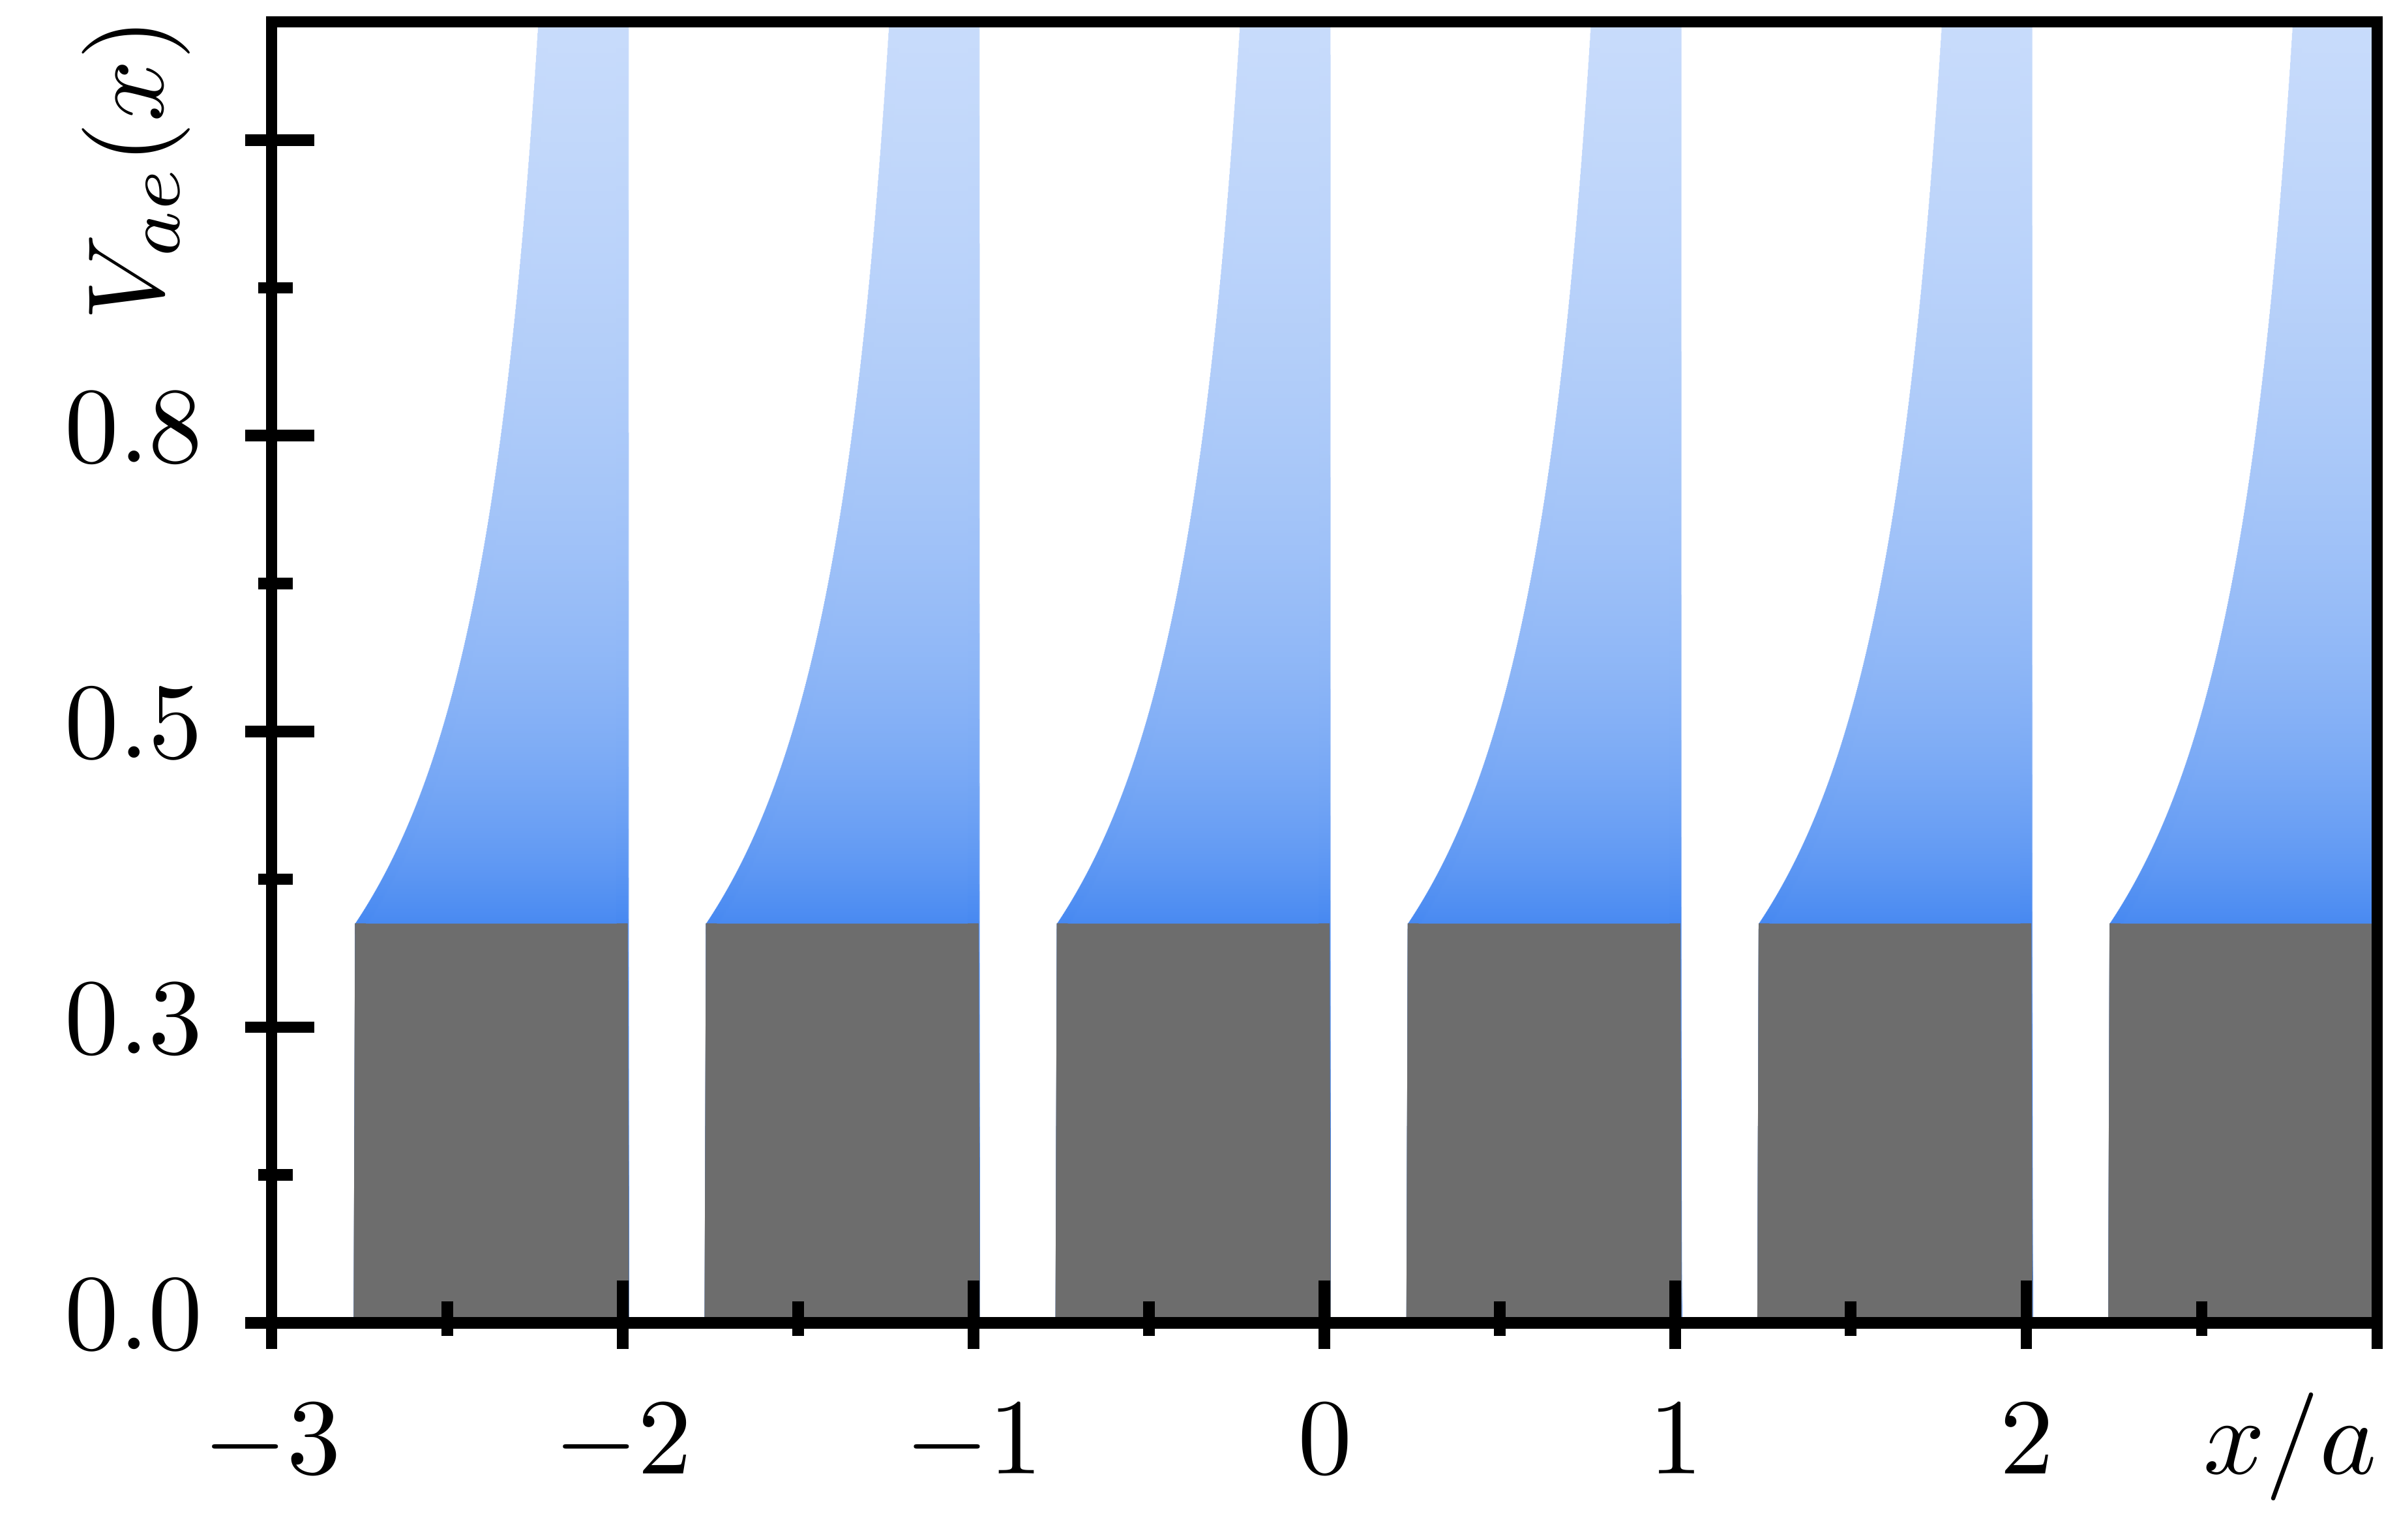
\includegraphics{figures/kronig_penney_potential.png}
    \caption{Contour of the periodic potential \cref{eq:kronig_penney_potential}. The shaded region in blue highlights the limits $b\rightarrow0$ and $V_0\rightarrow\infty$ while preserving a finite product $bV_0=P$ at all times.}
    \label{fig:kronig_penney_potential}
\end{figure}

% In order to preserve the periodicity of the potential, the system size must be commensurate to the lattice spacing $a$, i.e. $L\in a\mathds N$.
To simplify our problem, we can consider it to be a set of two different regions, i.e. (i) a free particle $-\frac{\hbar^2}{2m}\partial_x^2\psi_{\rm (i)}(x) = E\psi_{\rm (i)}(x)$ followed by (ii) a particle moving in a constant potential $-\frac{\hbar^2}{2m}\partial_x^2\psi_{\rm (ii)}(x) = (E-V_0)\psi_{\rm (ii)}(x)$.
In order to read-out the Bloch weights I conveniently factor a crystal momentum from the wave function
\begin{align}
    \psi_{\alpha k}^{\rm (i)}(x) = \re^{\ri kx}u_{\alpha k}^{\rm (i)}(x),
    \
    \psi_{\beta k}^{\rm (ii)}(x) = \re^{\ri kx}u_{\beta k}^{\rm (ii)}(x),
    \\
    u_{\alpha k}^{\rm (i)}(x) = A\re^{(\tau\alpha-\ri k) x} + A'\re^{-(\tau\alpha+\ri k) x},
    \
    u_{\beta k}^{\rm (ii)}(x) = B\re^{(\tau'\beta-\ri k) x} + B'\re^{-(\tau'\beta+\ri k) x},
\end{align}
with $\hbar^2\alpha^2 = 2m\abs{E}$, $\hbar^2\beta^2 = 2m\abs{(E-V_0)}$, $\tau^2=-\sign{E}$ and $\tau'^2=-\sign{E-V_0}$\footnote{Such that plane waves with $\tau=\tau'=\ri$ are obtained for $E>V_0$.}.
The wave functions are supposed to be smooth at the boundaries\footnote{I hereby use the notation of limits from above or below, i.e. $f(0^\pm)=\lim_{\epsilon\rightarrow0}f(\epsilon)$ for $\epsilon>0$.}, which results in
\begin{align}
    % \psi_{\alpha k}^{\rm (i)}(0^+)=\psi_{\beta k}^{\rm (ii)}(0^-),
    % \quad
    % {\psi_{\alpha k}^{\rm (i)}}'(0^+)={\psi_{\beta k}^{\rm (ii)}}'(0^-),
    % \\
    \psi_{\alpha k}^{\rm (i)}(-b+0^-)=\psi_{\beta k}^{\rm (ii)}(-b+0^+),
    \quad
    {\psi_{\alpha k}^{\rm (i)}}'(-b+0^-)={\psi_{\beta k}^{\rm (ii)}}'(-b+0^+),
\end{align}
and the Bloch functions inherit the potential's periodicity
\begin{align}
    u_{\alpha k}^{\rm (i)}(a+0^+) = u_{\alpha k}^{\rm (ii)}(0^-),
    \quad
    u_{\alpha k}^{\rm (i)}{}'(a+0^+) = u_{\alpha k}^{\rm (ii)}{}'(0^-).
\end{align}
In summary, the following matrix equation is derived
\begin{align}
    M=\begin{pmatrix}
        1 & 1 & -1 & -1\\
        %
        \tau\alpha & -\tau\alpha & -\tau'\beta & \tau'\beta\\
        %
        \re^{(\tau \alpha-\ri k)(a-b)}  & \re^{-(\tau \alpha+\ri k) (a-b)} &
        -\re^{-(\tau'\beta -\ri k)b}     & -\re^{ (\tau'\beta+\ri k)b} \\
        %
        (\tau \alpha-\ri k)\re^{(\tau \alpha-\ri k)(a-b)}  & -(\tau \alpha+\ri k)\re^{-(\tau \alpha+\ri k) (a-b)} &
        -(\tau'\beta -\ri k)\re^{-(\tau'\beta -\ri k)b}     & (\tau'\beta+\ri k)\re^{ (\tau'\beta+\ri k)b} \\
    \end{pmatrix},
\end{align}
satisfying $M(A,A',B,B')^T=0$.
For nontrivial results, the determinant of $M$ should be equal to zero, which is satisfied for solutions of the transcendental equation
\begin{align}
    \cos(ka)
    =
    \cosh(\alpha\tau(a-b))\cosh(b\beta\tau')
    +
    \frac{\alpha^2\tau^2+\beta^2\tau'^2}{2\alpha\beta\tau\tau'}\sinh(\alpha\tau(a-b))\sinh(b\beta\tau).
    \label{eq:kronig_penney_transcendental_equation}
\end{align}
To approximate the right hand side in the aforementioned limits, application of
\begin{align}
    b\rightarrow0,
    \quad
    V_0\rightarrow\infty,
    \quad
    bV_0 = {\rm constant}
    \\
    \Rightarrow
    b\beta^2\rightarrow 2mbV_0/\hbar^2,
    \quad
    \cosh(b\beta\tau')\rightarrow 1,
    \quad
    \sinh(b\beta\tau')\rightarrow b\beta\tau'
\end{align}
provides an exact solution of \cref{eq:kronig_penney_transcendental_equation} in the limit of narrow and strong periodic potentials\footnote{This limit is actually equivalent to a potential composed by delta-distributions.}
\begin{align}
    f(\alpha a) = \cosh(\alpha\tau a) + \tau'^2\frac{P}{\alpha\tau a}\sinh(\alpha\tau a),
    \quad
    P=mabV_0/\hbar^2.
    \label{eq:kronig_penney_transcendental_equation_approx}
\end{align}
If we assume bound states between the potential wells $0<E<V_0$, the signs become $\tau^2=-1$ and $\tau'^2=+1$, such that \cref{eq:kronig_penney_transcendental_equation_approx} evaluates to
\begin{align}
    f(\alpha a) = \cos(\alpha a) + \frac{P}{\alpha a}\sin(\alpha a).
    \label{eq:kronig_penney_transcendental_equation_approx_bound}
\end{align}
The right-hand-side of \cref{eq:kronig_penney_transcendental_equation_approx_bound} is in general not bound to the interval $[-1,+1]$ spanned by $\cos(ak)$ and establishes values of $\alpha$ (thus, the square-root of the energy $E$) for which no (real) momentum exists (see \cref{fig:kronig_penney_dispersion} (a)).
Such energies are called forbidden and realize a first understanding of band-gaps induced by the nonzero lattice potential $V_0>0$.
\\

If $P=0$, we are left with the energy-momentum relation of free electrons $k=\alpha$ and thus $E_0={\hbar^2k^2}/({2m})$.
If we approach $P\rightarrow\infty$, the allowed energies are formed by the roots of $f$, which are given by the dominating term and yield discretized energies
\begin{align}
    E_{\infty,n_b}=(\hbar n_b\pi)^2/(2ma^2)
    \label{eq:kronig_penney_energy_tb}
\end{align}
spanned by integer numbers ($n_b=1,2,\dots$).
The intermediate regimes $0<P<\infty$ can be solved by numerical evaluation of \cref{eq:kronig_penney_transcendental_equation_approx_bound} and are plotted in \cref{fig:kronig_penney_dispersion} (a).
Straightforward evaluation of $\arccos(f)$ evaluates the crystal momentum $ka$ and yields the so-called ``reduced zone scheme'' displayed in \cref{fig:kronig_penney_dispersion} (b).
\\

To get an analytic understanding of the wave functions in the above limit, let's focus on the region without potential (i) [$b$ is sent to zero anyhow]
\begin{align}
    \psi_{\alpha k}^{\rm (i)}(x) = \re^{\ri kx}u_{\alpha k}^{\rm (i)}(x),
    \quad
    u_{\alpha k}^{\rm (i)}(x) = A\re^{\ri(\alpha-k) x} + A'\re^{-\ri(\alpha+k) x},
    \quad
    u_{\alpha k}^{\rm (i)}(x+na)=u_{\alpha k}^{\rm (i)}(x)
    \label{eq:kronig_penney_wavefunctions}
\end{align}
in which the prefactors are related by\footnote{An additional constraint for $AA^*$ is found by requiring normalization of the wave functions, which allows to compute expectation values. However, it is not needed for the purpose of this section and I refer to \cite{KronigPenney1931}.}
\begin{align}
    A' = -A\frac{1-\re^{\ri(\alpha-k)a)}}{1-\re^{-\ri(\alpha+k)a}}.
    \label{eq:kronig_penney_constants}
\end{align}
Starting from \cref{eq:kronig_penney_transcendental_equation_approx_bound}, we see that for any solution $\alpha a$ satisfying $f(\alpha a)=\cos(k a)$ there are an infinite number of symmetric points in momentum space which fulfill the same equation, i.e. (a) $ka + 2n\pi$ and (b) $-ka+2n\pi$.
Close inspection of \cref{eq:kronig_penney_wavefunctions,eq:kronig_penney_constants} reveals that a transformation according to (a) leaves the wave function invariant, while (b) maps it to the solutions of $-ka$, $-\alpha a$.
In other words, (a) is merely a shift by a unit reciprocal vector and (b) flips the direction of the propagating wave, hence establishes a mirror symmetry at the $ka=0$ axis which is a consequence of the system being invariant under time-reversal.
The properties (a) and (b) allow to define the ``unfolding'' of the reduced zone scheme:
without loss of generality, a crystal momentum $n_b\pi\leq ka<(n_b+1)\pi$ can be uniquely connected to an energy value $n_b\pi\leq \alpha a<(n_b+1)\pi$ by introducing a band index $(n_b=0,1,\dots)$.
Here, the limit of free particles ($P=0$) is readily restored, since \cref{eq:kronig_penney_constants} vanishes for $\alpha a = ka$ [except for the special points $ka=n_b\pi$].
At the special points, \cref{eq:kronig_penney_constants} is actually ill defined and evaluates to the two viable solutions $A'=\pm A$, which can be understood from the two non-commuting limits
\begin{align}
    -\lim_{\alpha a \searrow n_b\pi}\frac{1-\re^{\ri(\alpha a-n_b\pi))}}{1-\re^{-\ri(\alpha a+n_b\pi)}}
    =
    -\lim_{\epsilon\searrow0}\frac{1-\re^{+\ri\epsilon}}{1-\re^{-\ri\epsilon}}
    =
    \lim_{\epsilon\searrow0}\re^{+\ri\epsilon}\frac{1-\re^{-\ri\epsilon}}{1-\re^{-\ri\epsilon}}
    =
    +1,
    \\
    -\lim_{k a \searrow n_b\pi}\frac{1-\re^{\ri(n_b\pi - ka))}}{1-\re^{-\ri(n_b\pi+ka)}}
    =
    -\lim_{k a \searrow n_b\pi}\frac{1-\re^{-\ri(n_b\pi + ka))}}{1-\re^{-\ri(n_b\pi+ka)}}
    =
    -1.
\end{align}
The two allowed eigenfunctions are standing waves $\propto \cos(kx),\sin(kx)$.
By reformulating the special points in terms of the particles de Broglie wavelength $\lambda=2\pi/k$, the formation of standing waves can be understood as a residual effect of (constructive) Bragg reflection on a periodic grid structure.
Standing waves are obtained if the particle's de Broglie wavelength and the spacing of the potential satisfy $2a=n_b\lambda$.
\begin{figure}
    \centering
    \subfigure[]{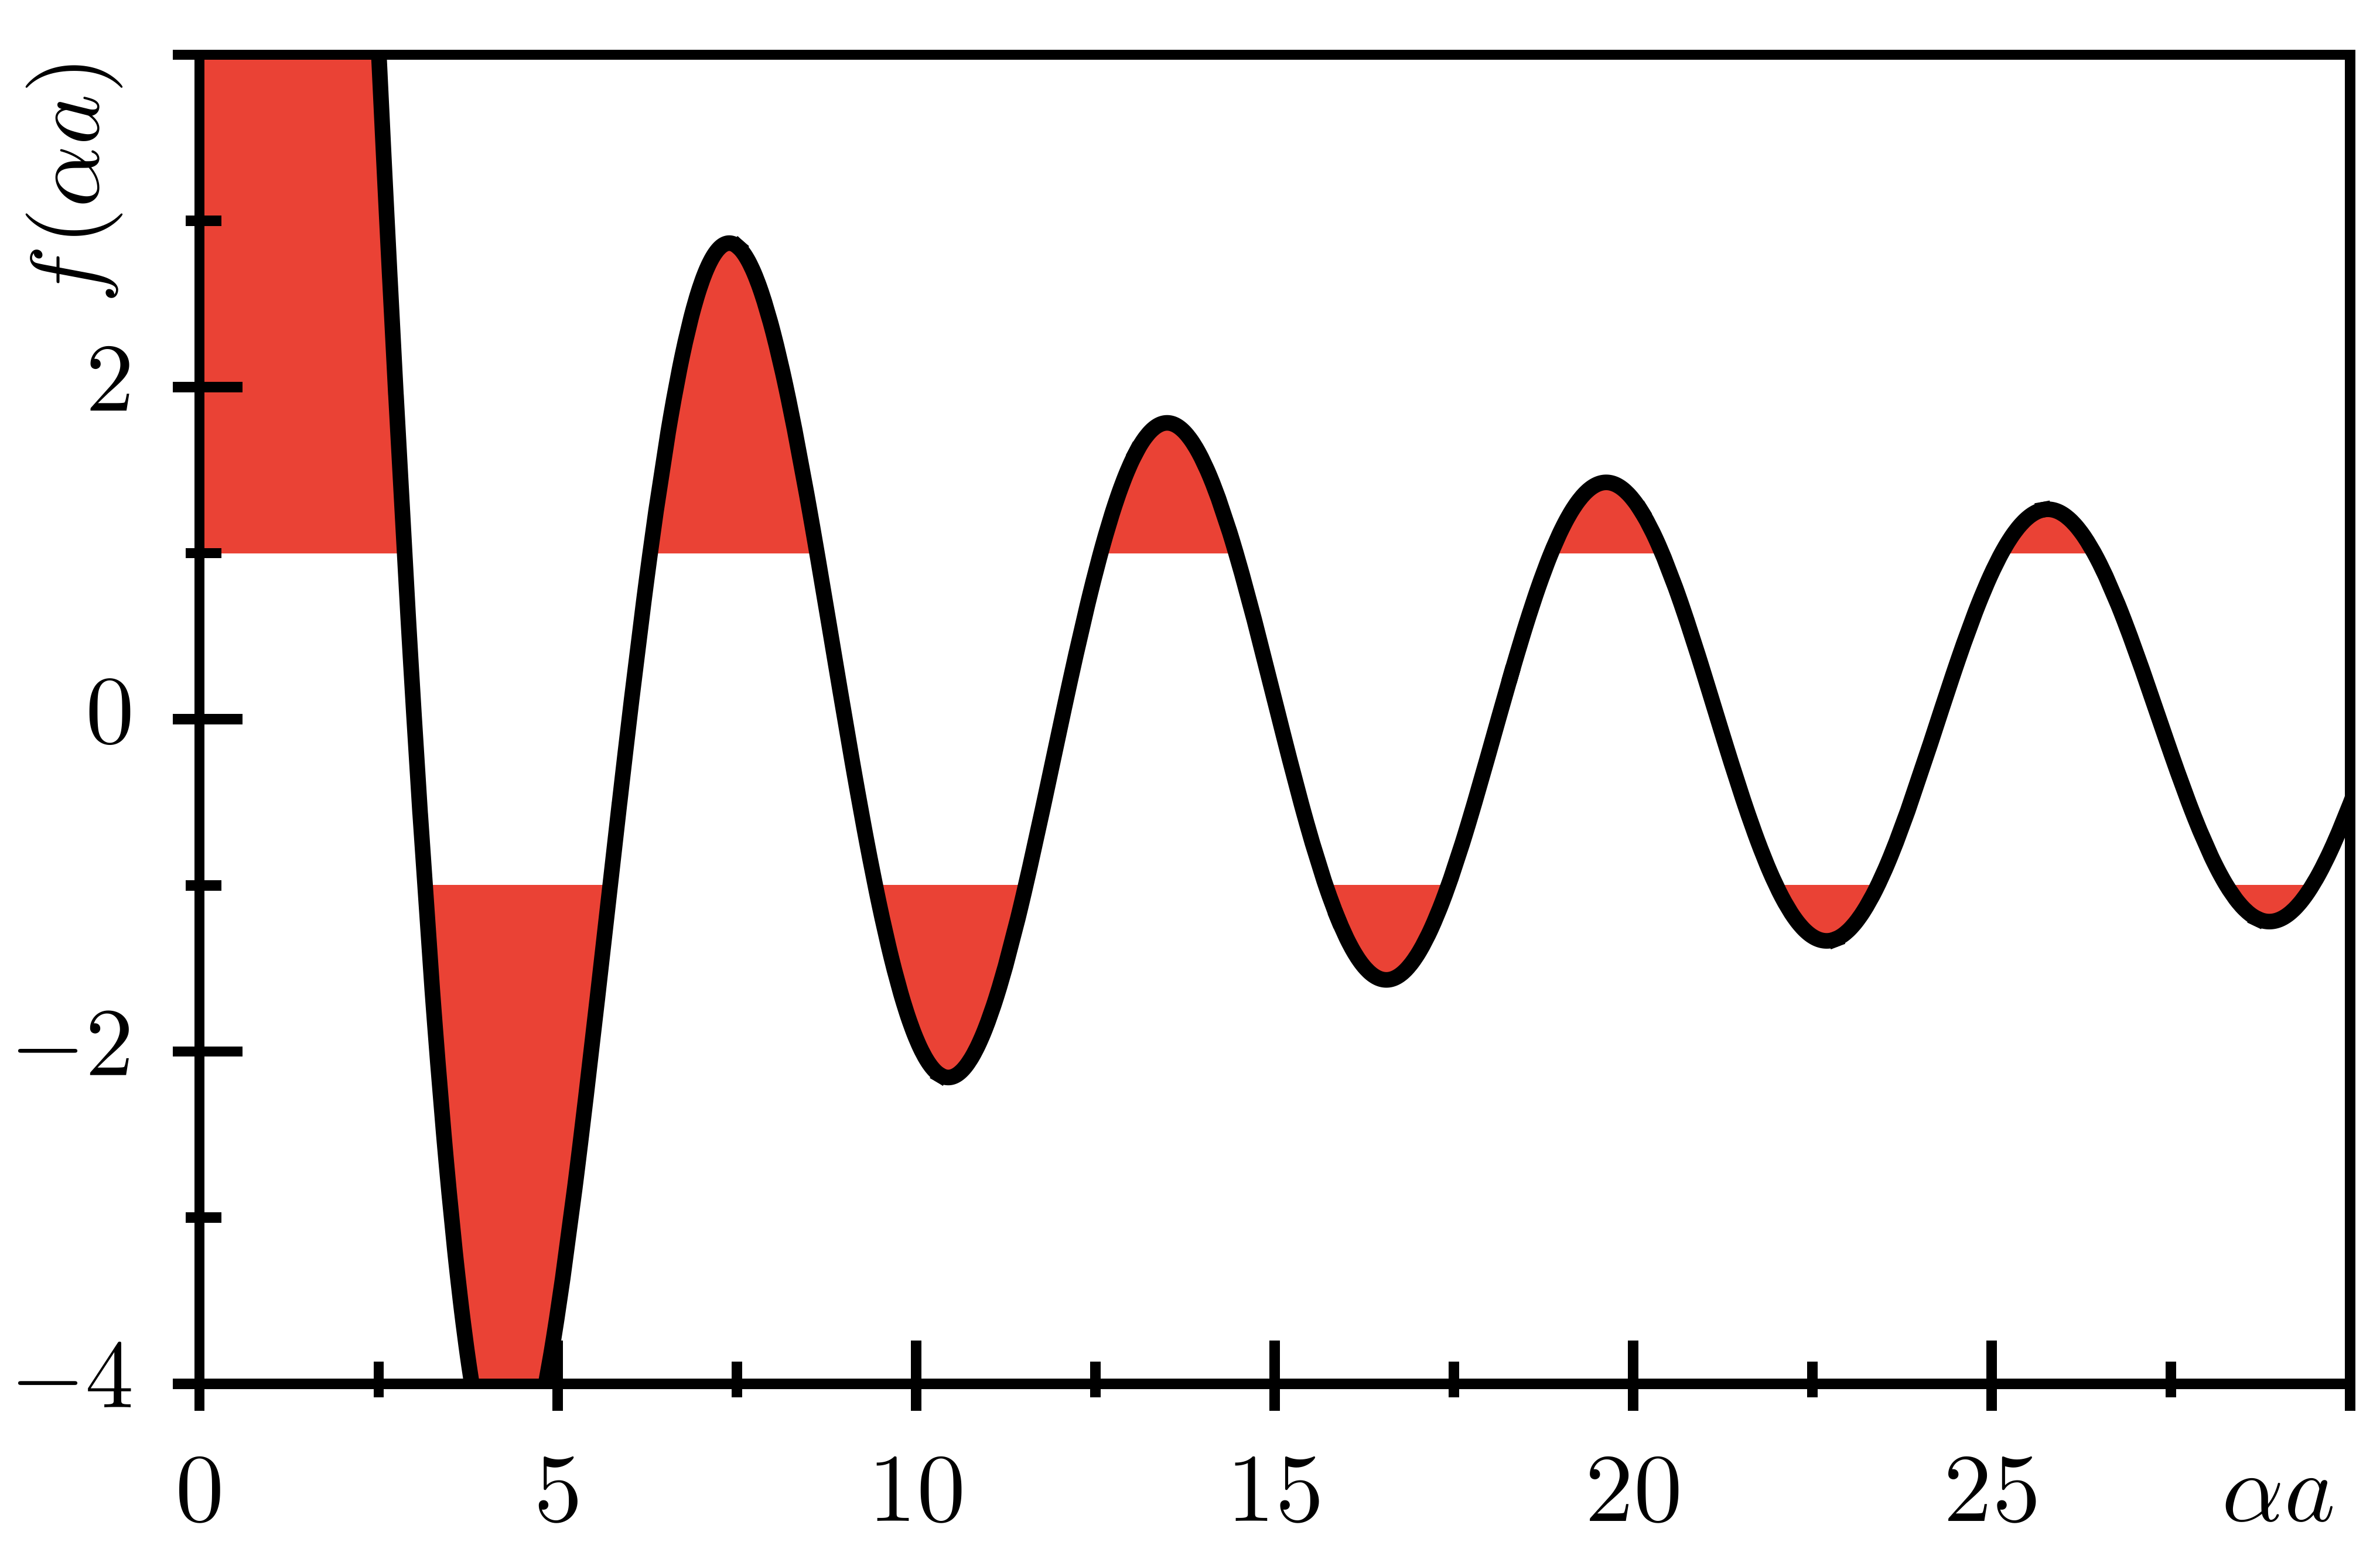
\includegraphics{figures/kronig_penney_transcendental.png}}
    \subfigure[]{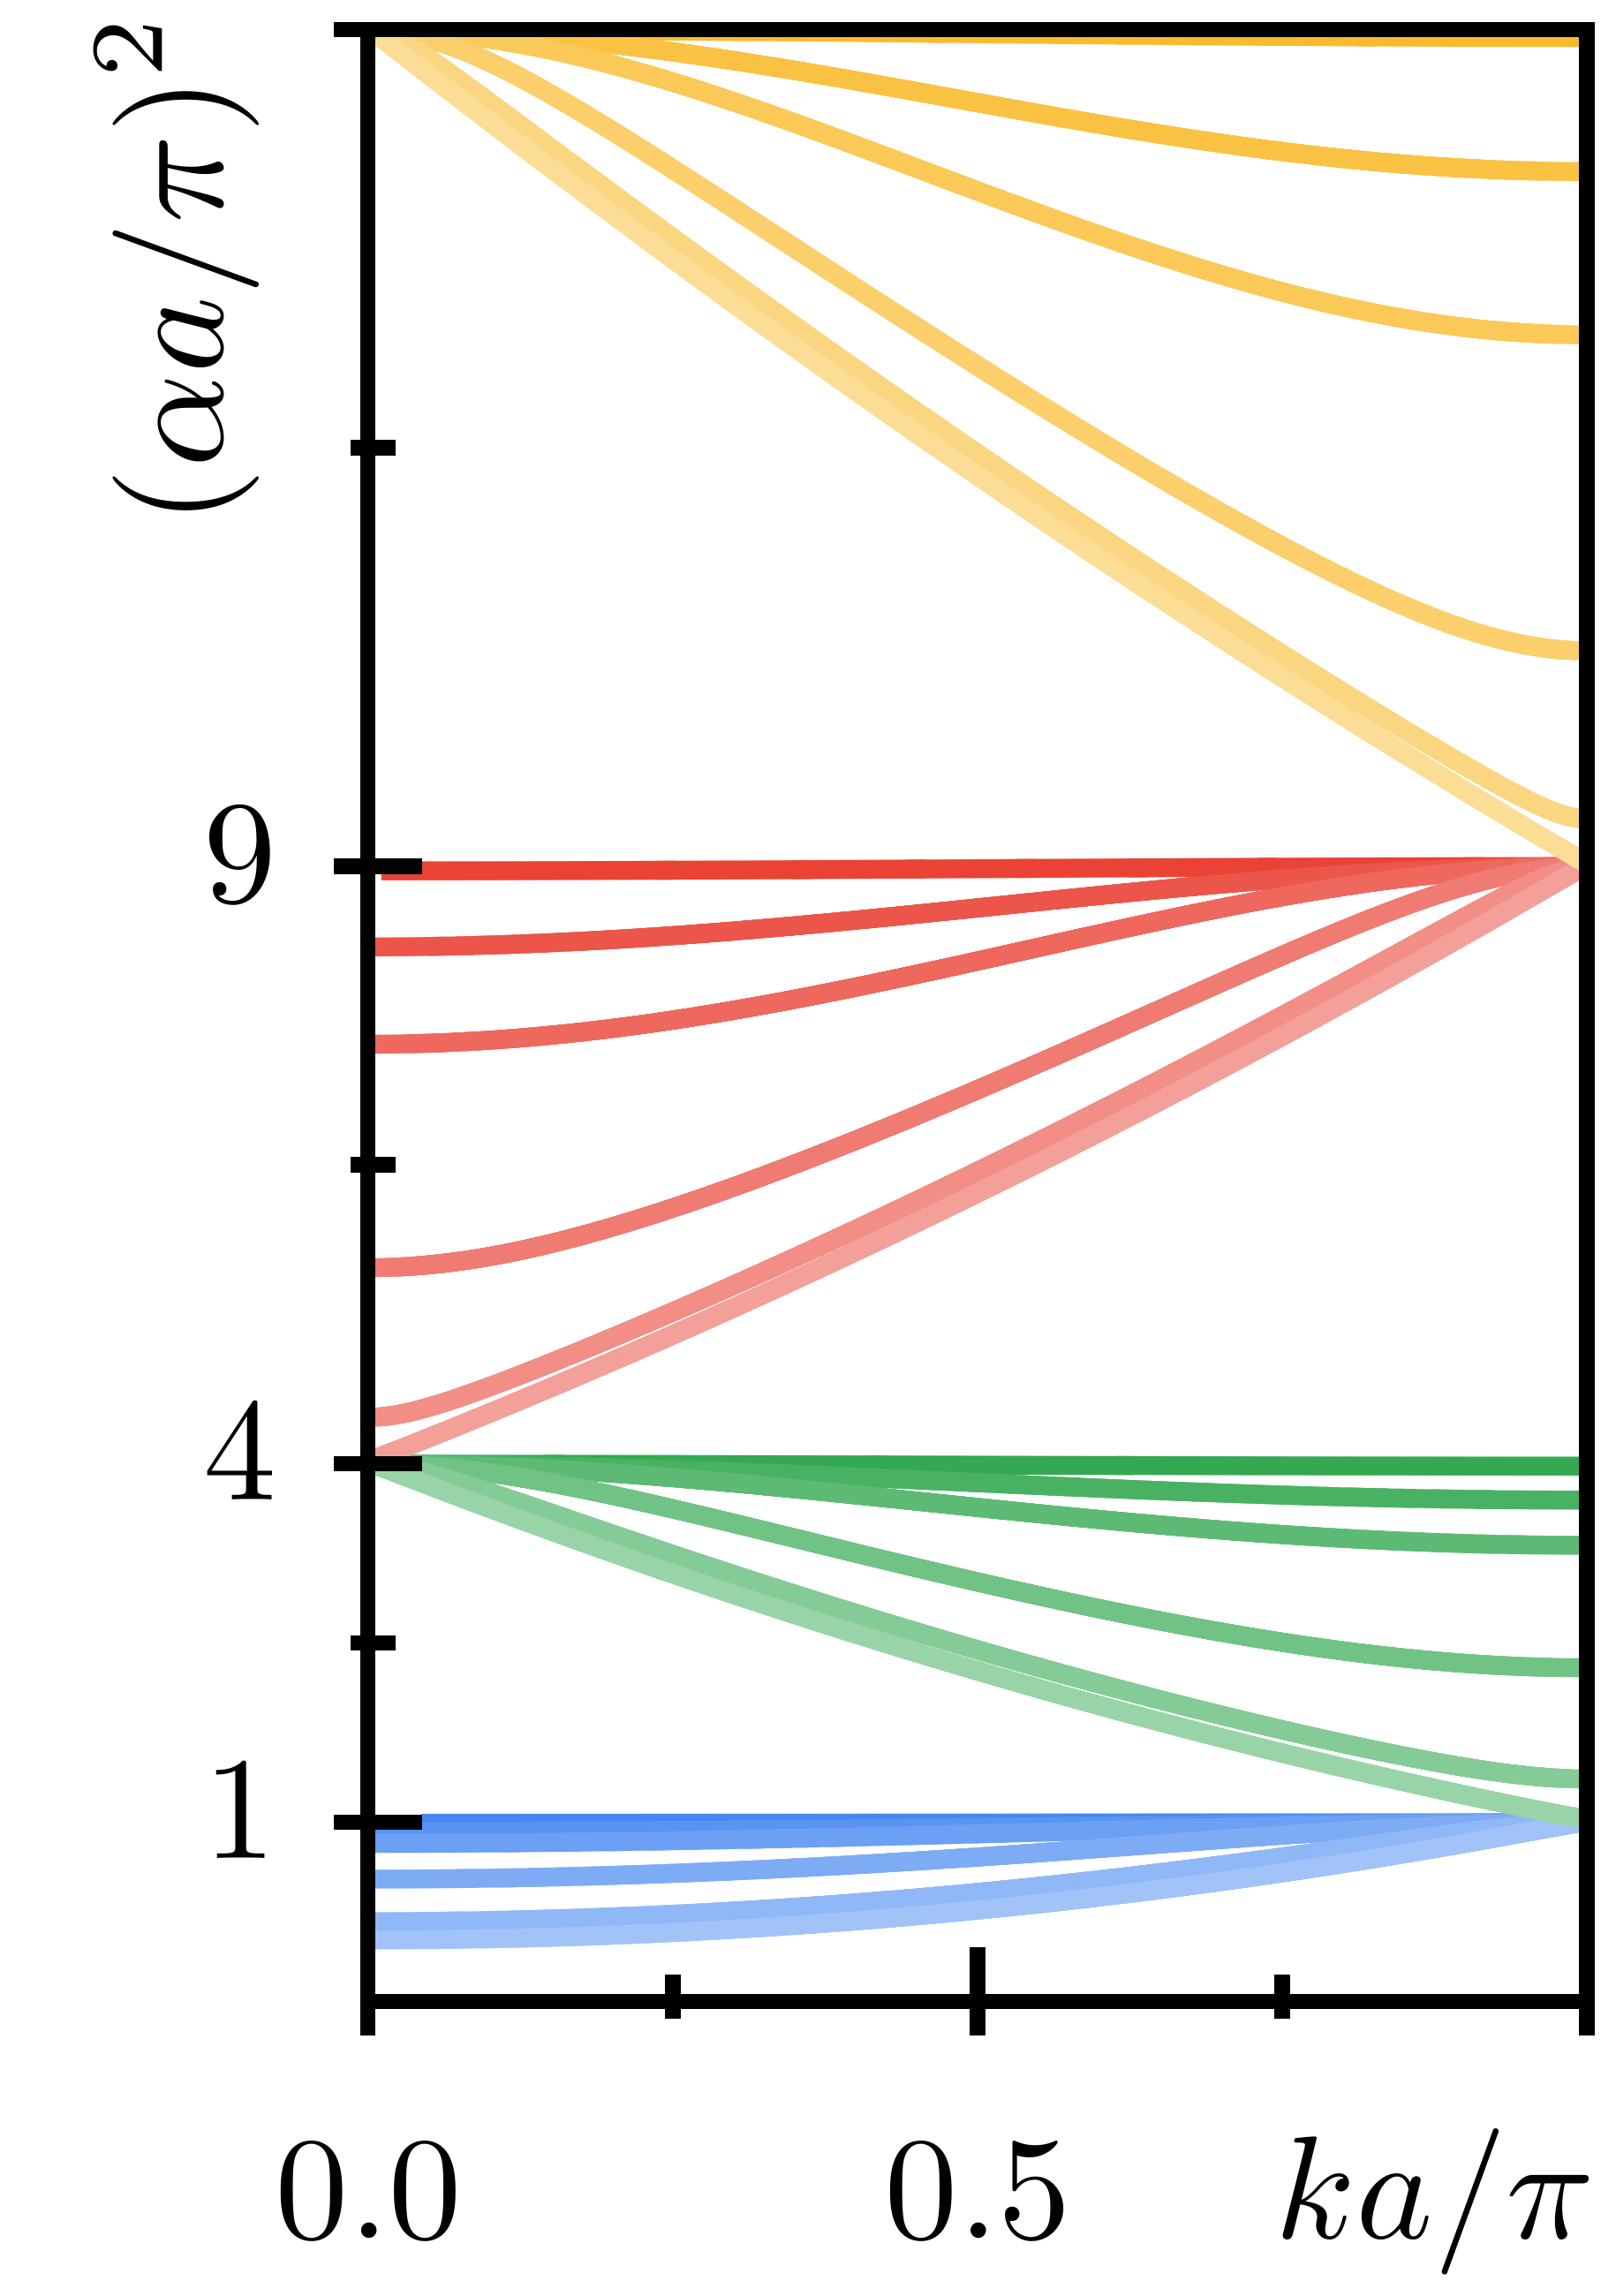
\includegraphics{figures/kronig_penney_dispersion_2.png}}
    \subfigure[]{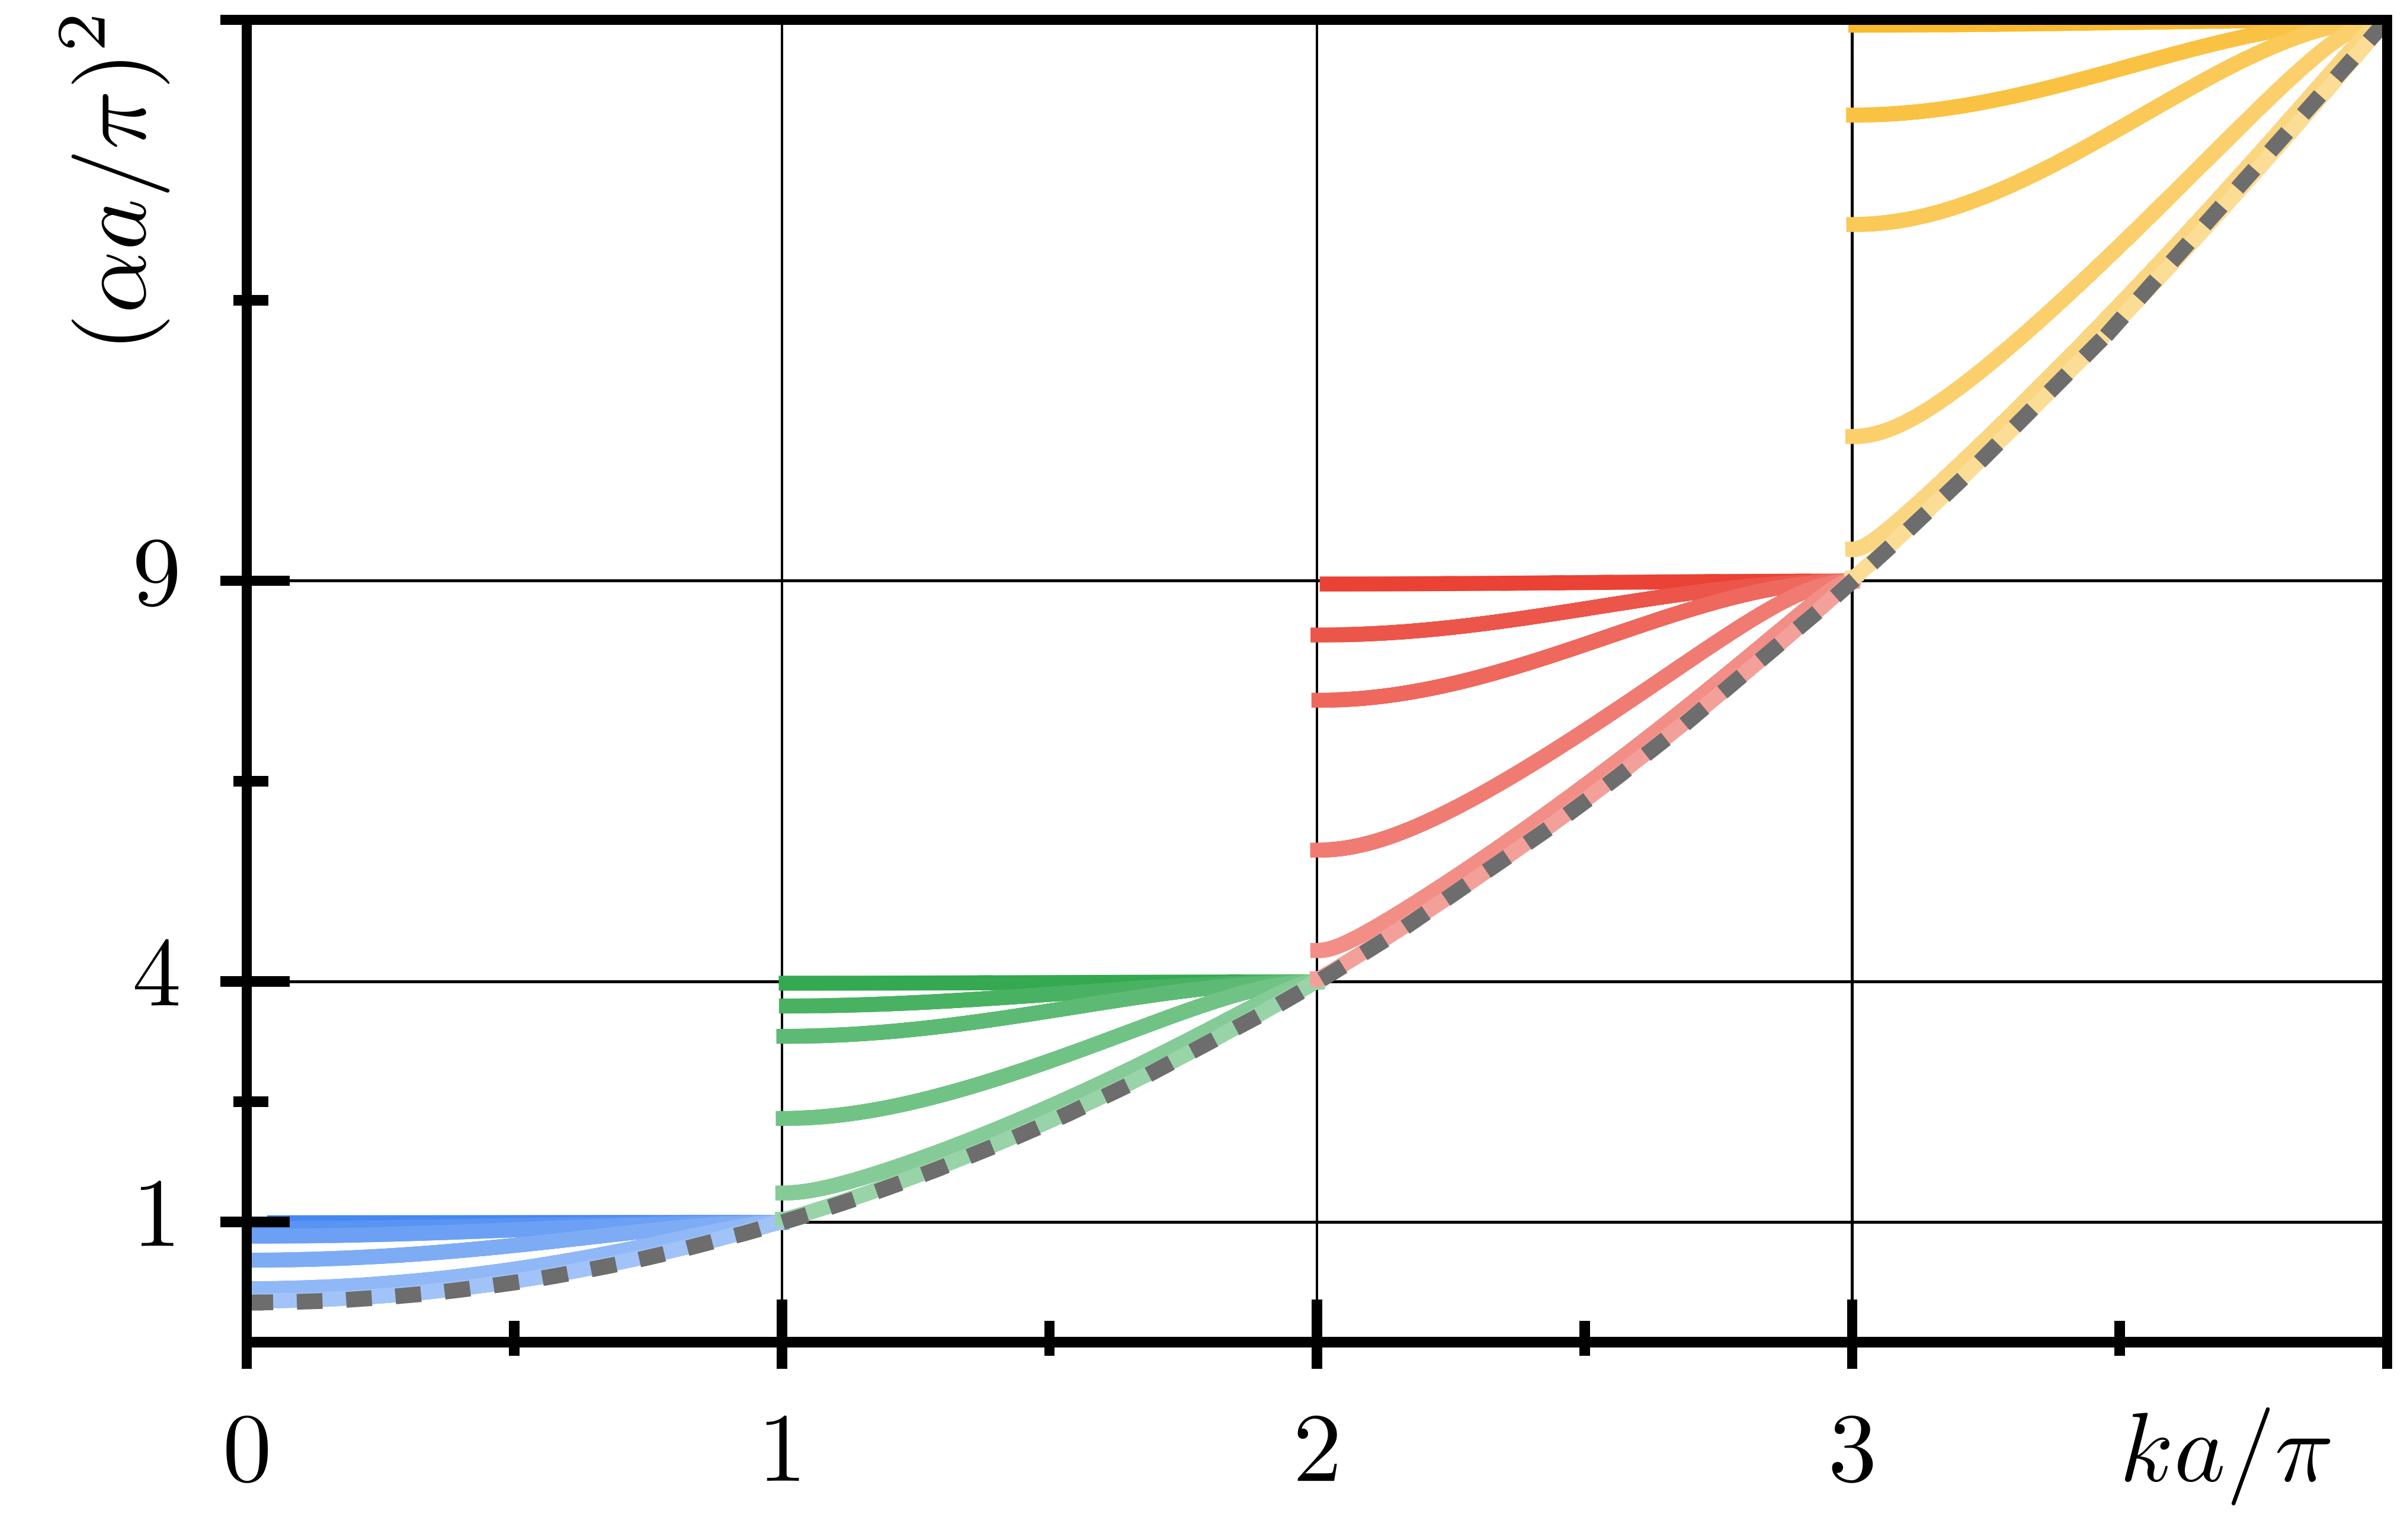
\includegraphics{figures/kronig_penney_dispersion_1.png}}
    \caption{
    (a) Plot of the right-hand-side of the transcendental equation. Solutions do not exist in the red regions.
    (b)-(c) Shapes of the dispersion relation $(\alpha a/\pi)^2$ versus crystal momentum $ka/\pi$ given by \cref{eq:kronig_penney_transcendental_equation_approx_bound}.
    Different opacity (transparent to colors) represent increasing values of $P\in\{0.1,1,5,20,50,1000\}$.
    (c) The properties of the wave functions allow to uniquely relate the crystal momentum $ka$ to an energy $\alpha a$ in which the limit of free electrons [i.e. $P\rightarrow0$] is pronounced.}
    \label{fig:kronig_penney_dispersion}
\end{figure}

In the limit $P\rightarrow\infty$, the energy $E_{\infty,n_b}$ assumes the discrete values in \cref{eq:kronig_penney_energy_tb} resulting in motionless eigenstates -- the resulting waves are tightly bound to the potential minimum.
If we relax this limit a bit, i.e. $P\gg 1$, a reasonable approximation of the lowest band curvature is obtained by a first order Taylor series of \cref{eq:kronig_penney_transcendental_equation_approx_bound} resulting in the typical dispersion relation for tight binding systems, i.e.
\begin{align}
    E_{P\gg1,1}\approx t_0 + t_1 \cos(k a),
    \quad
    t_0 = + E_{\infty,1} - \frac{\pi^2 \hbar^4}{a^3 m^2 b V_0},
    \quad
    t_1 = -\frac{\pi^2\hbar^4}{a^3 m^2 bV_0}.
    \label{eq:kronig_penney_tight_binding_dispersion}
\end{align}

A way to numerically solve generic potentials is obtained by expanding the Schrödinger equation in reciprocal space through the following identities\footnote{The reciprocal space provides a way to Fourier-transform as the functions $\re^{\ri {\bf G r}}$ form a basis on the primitive cell of the real lattice over the square-integrable functions. In particular, the functions satisfy the orthogonality equation $\delta_{\bf G, G'}=\frac1{\Omega}\int\rd^dr\,\re^{\ri({\bf G-G'}){\bf r}}$.}
\begin{align}
    V_{ae}({\bf r}) = \sum_{\bf G}V_{ae}{}_{\bf G}\re^{\ri {\bf G r}},
    \quad
    V_{ae}{}_{\bf G} = \frac1{V}\int\rd^dr\,V_{ae}({\bf r}){\bf G}\re^{-\ri {\bf G r}},
    \\
    u_{n{\bf k}}({\bf r}) = \sum_{\bf G}u_{n{\bf k}}({\bf r}){}_{\bf G}\re^{\ri {\bf G r}},
    \quad
    u_{n{\bf k}}({\bf r}){}_{\bf G} = \frac1{V}\int\rd^dr\,u_{n{\bf k}}({\bf r})\re^{-\ri {\bf G r}},
\end{align}
in which $V$ is the volume of the primitive unit cell.
Straightforward evaluation yields the algebraic eigenvalue problem for the unknown functions $u_{n{\bf k}}{}_{\bf G}$
\begin{align}
    \frac{\hbar^2}{2m}({\bf G}+{\bf k})^2u_{n{\bf k}}{}_{\bf G}+\sum_{\bf G'}V_{ae}{}_{\bf G-G'}u_{n{\bf k}}{}_{\bf G'} = E_{n{\bf k}}.
    \label{eq:periodic_lattices_numerics}
\end{align}
The dimension of the linear equation is infinite due to the sum over all reciprocal lattice vectors and has to be truncated if one wants to solve the equation numerically [the convergence of such a truncation has to be carefully checked for a serious investigation].
Clearly, strongly confined potentials such as delta functions are particularly bad candidates to solve numerically through evaluation of \cref{eq:periodic_lattices_numerics} because the resulting matrix equation will not be sparse and any truncation will have a significant error.
%
%
%%%%%%%%%%%%%%%%%%%%%%%%%%%%%%%%%%
\section{Tight binding systems}
\label{sec:tight_binding_systems}
%%%%%%%%%%%%%%%%%%%%%%%%%%%%%%%%%%
The systems considered here are those of tightly bound constituents to the lattice centers.
Such types can be found in traditional solid state scenarios where the nuclei are well separated beyond the typical Bohr radius of the valence electrons, in setups of ultracold atoms trapped in optical lattices, in optical waveguides or polaritons.
In \cref{part:results}, I will mostly cover theoretical aspects of tight binding models which can be experimentally realized in a variety of different setups.
For this reason, it will be useful to review briefly how these models are motivated in general from a more traditional solid state aspect, and how they can be understood in the more modern approach of second quantization.
\\

\begin{figure}
    \centering
    \subfigure[]{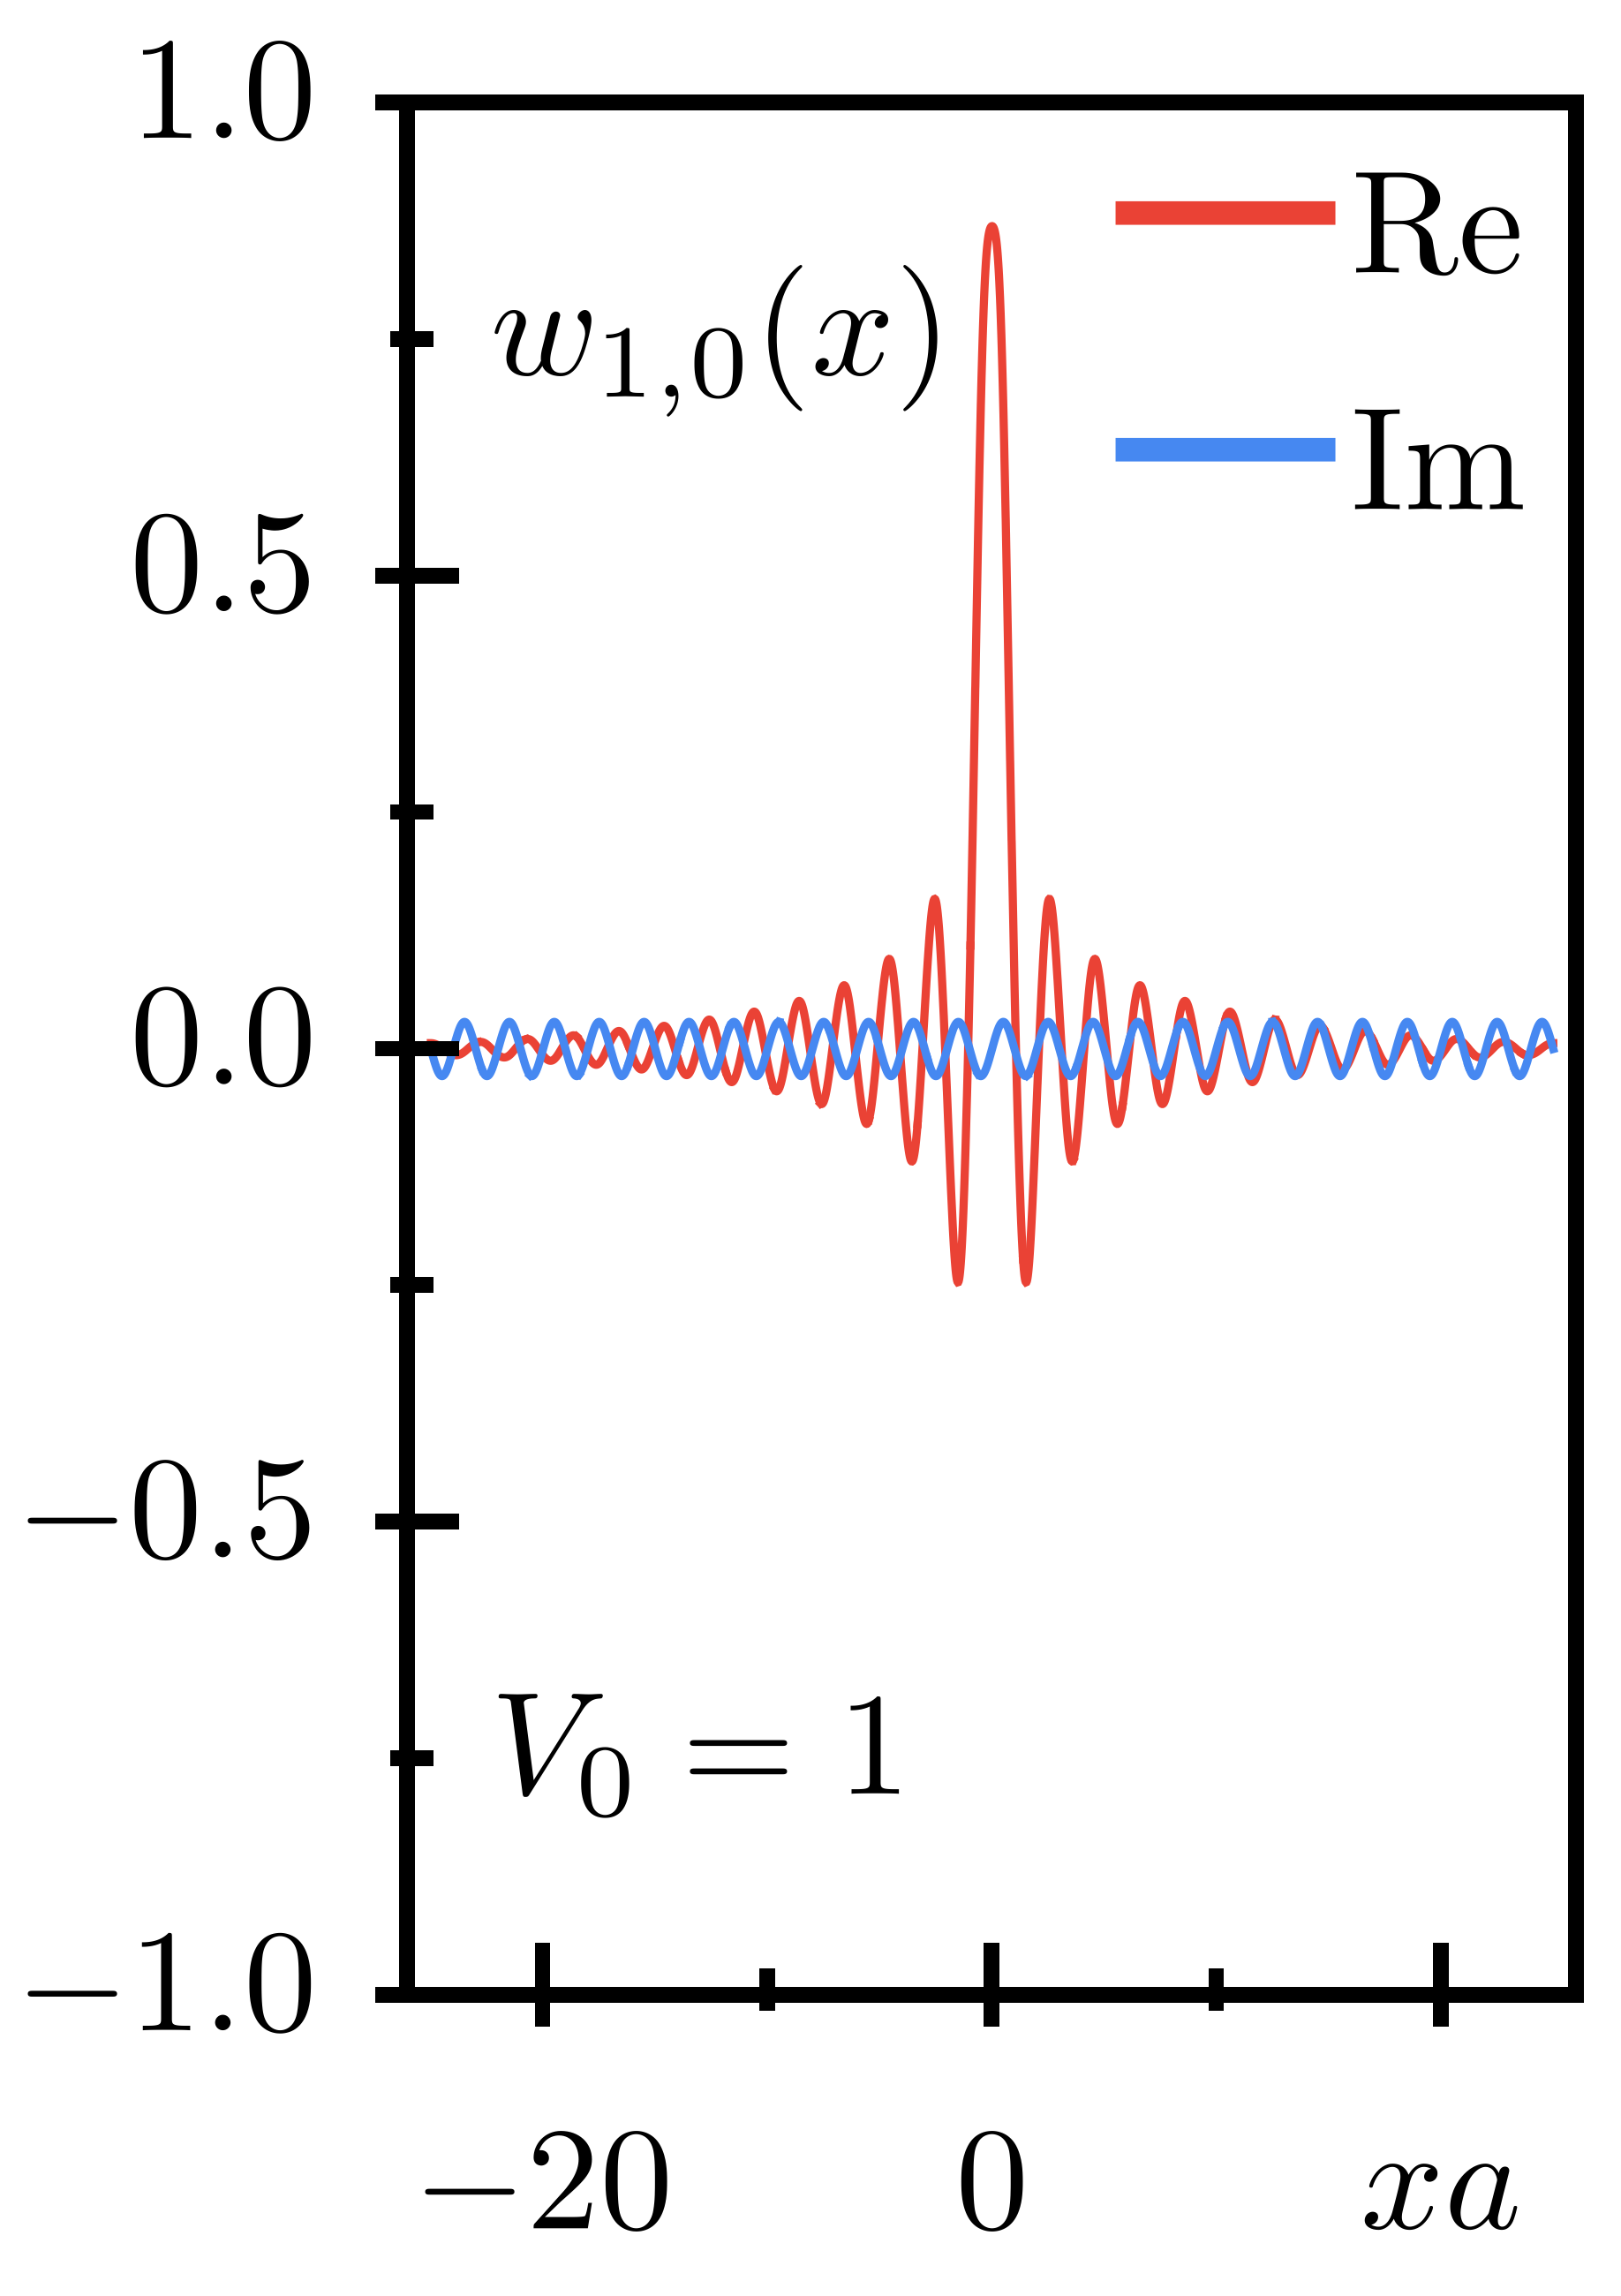
\includegraphics{figures/wannier1_1.png}}
    \subfigure[]{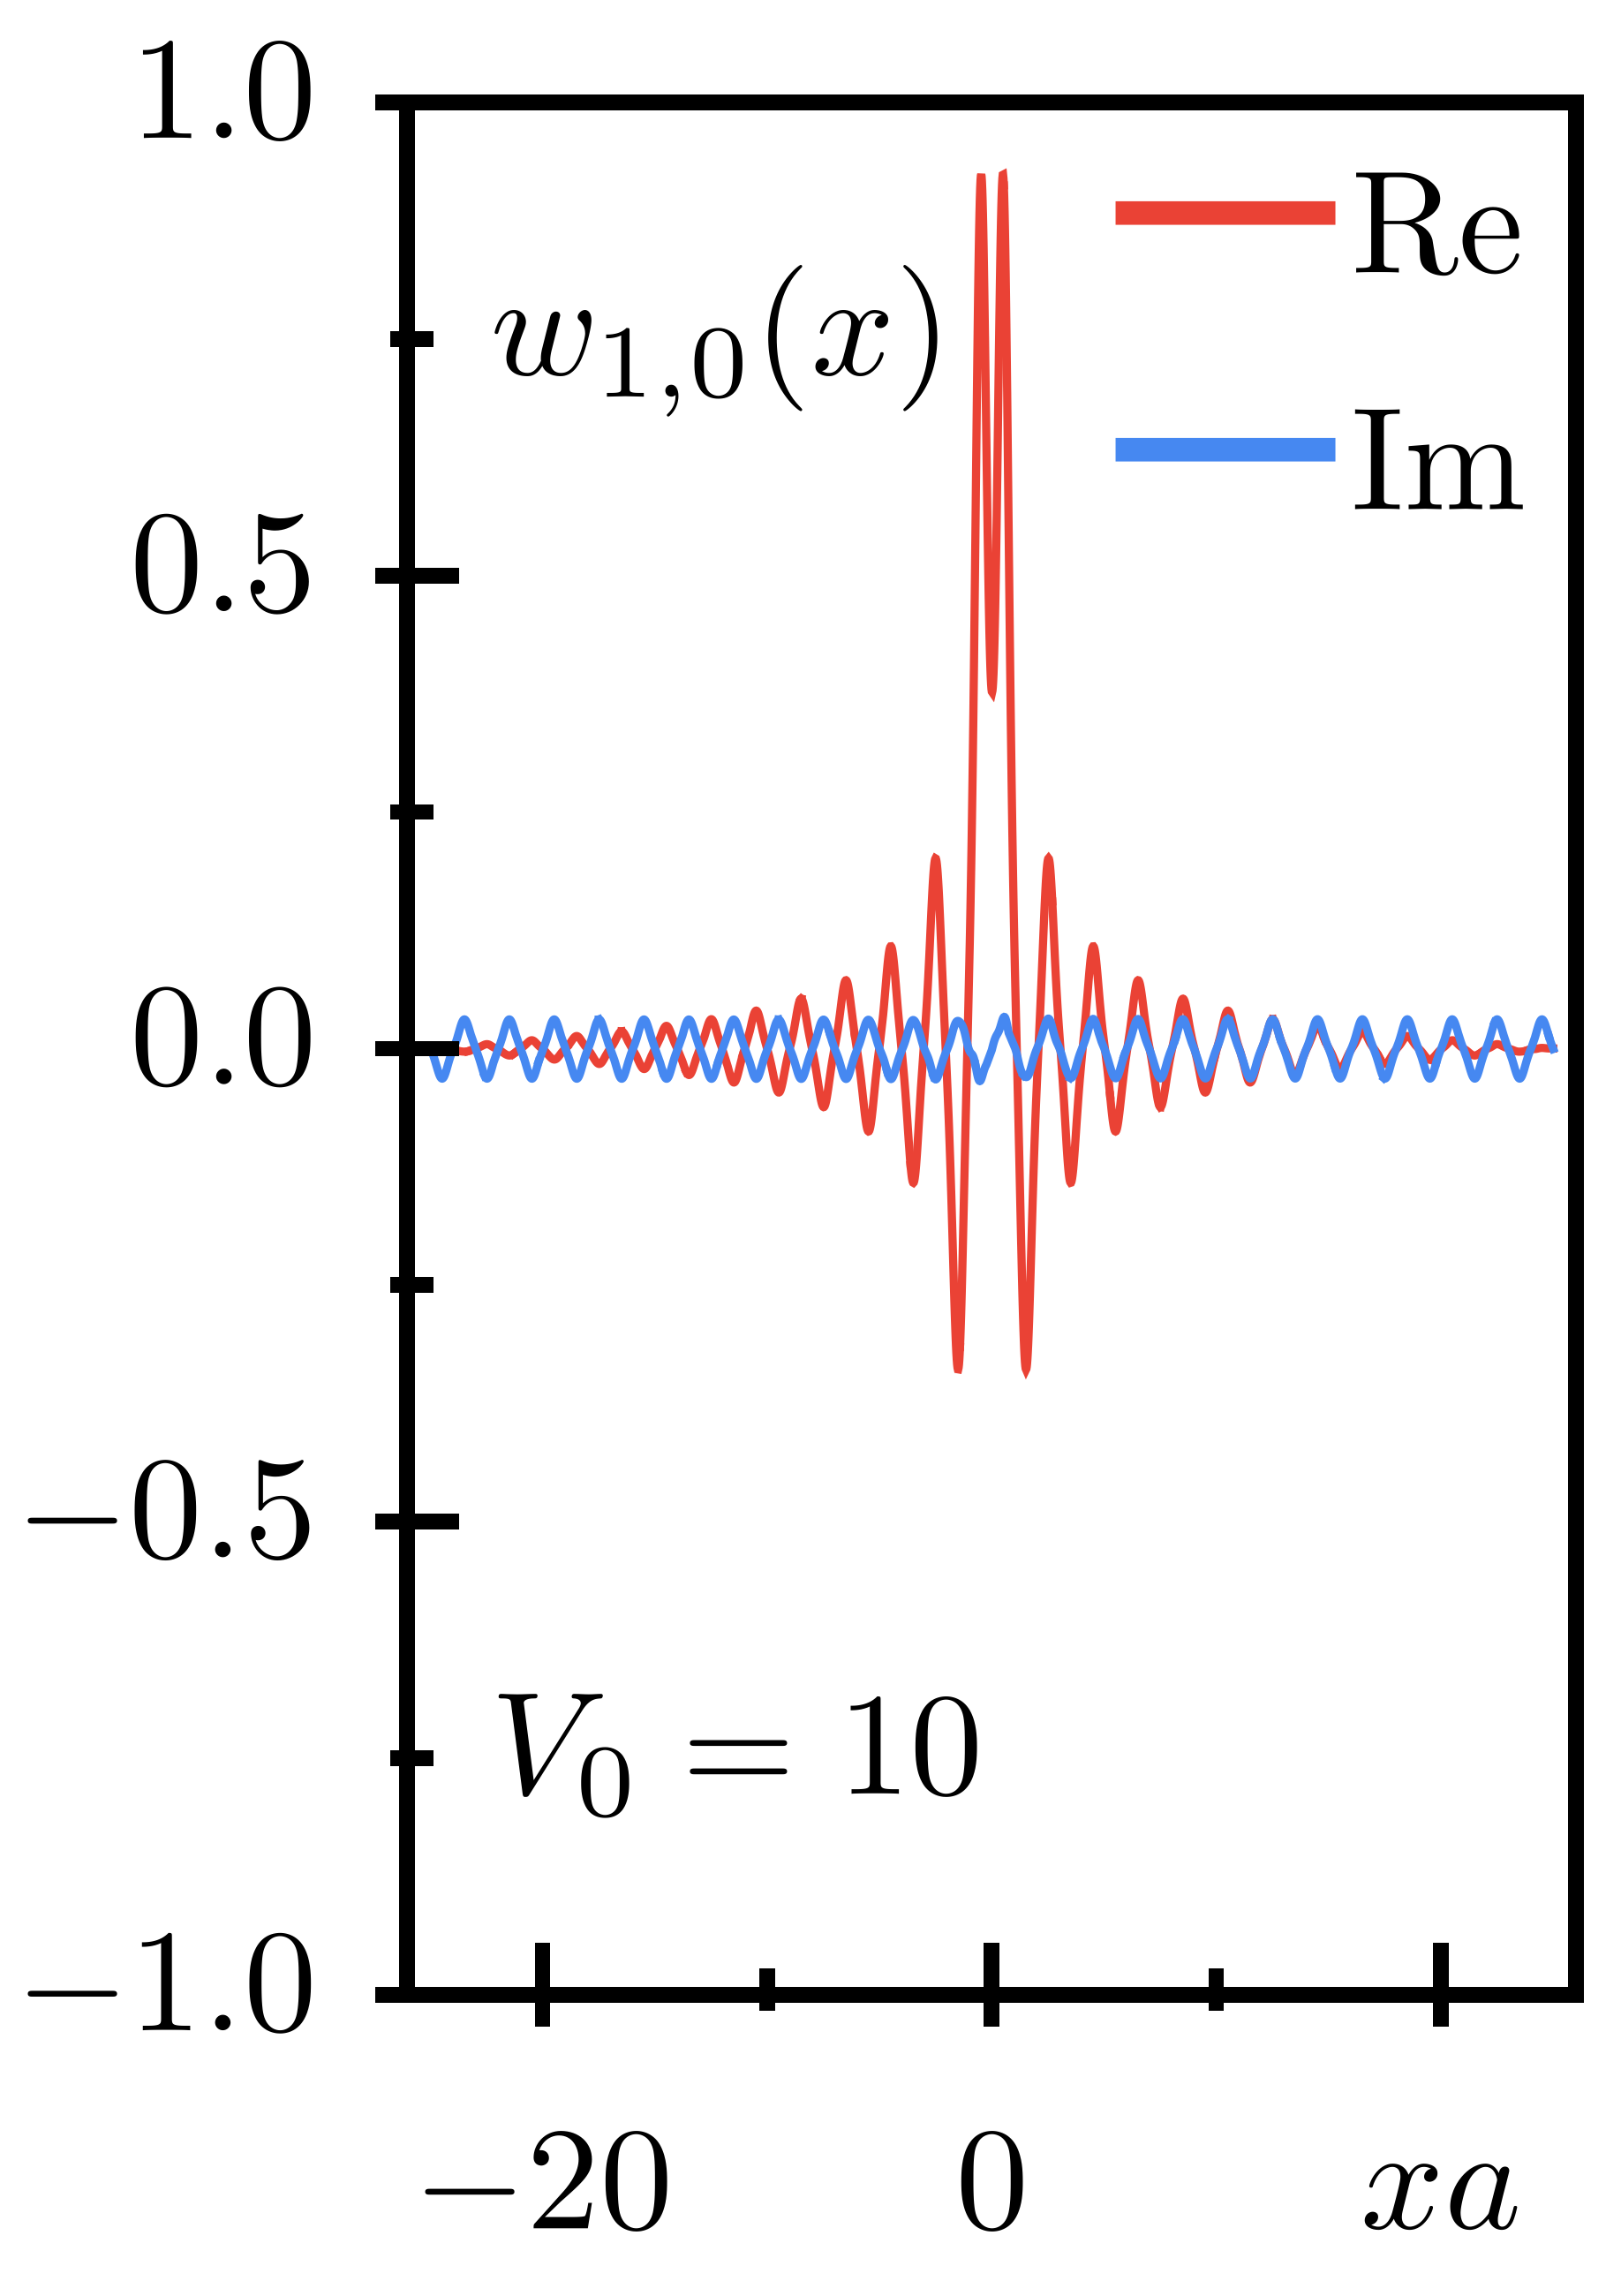
\includegraphics{figures/wannier1_10.png}}
    \subfigure[]{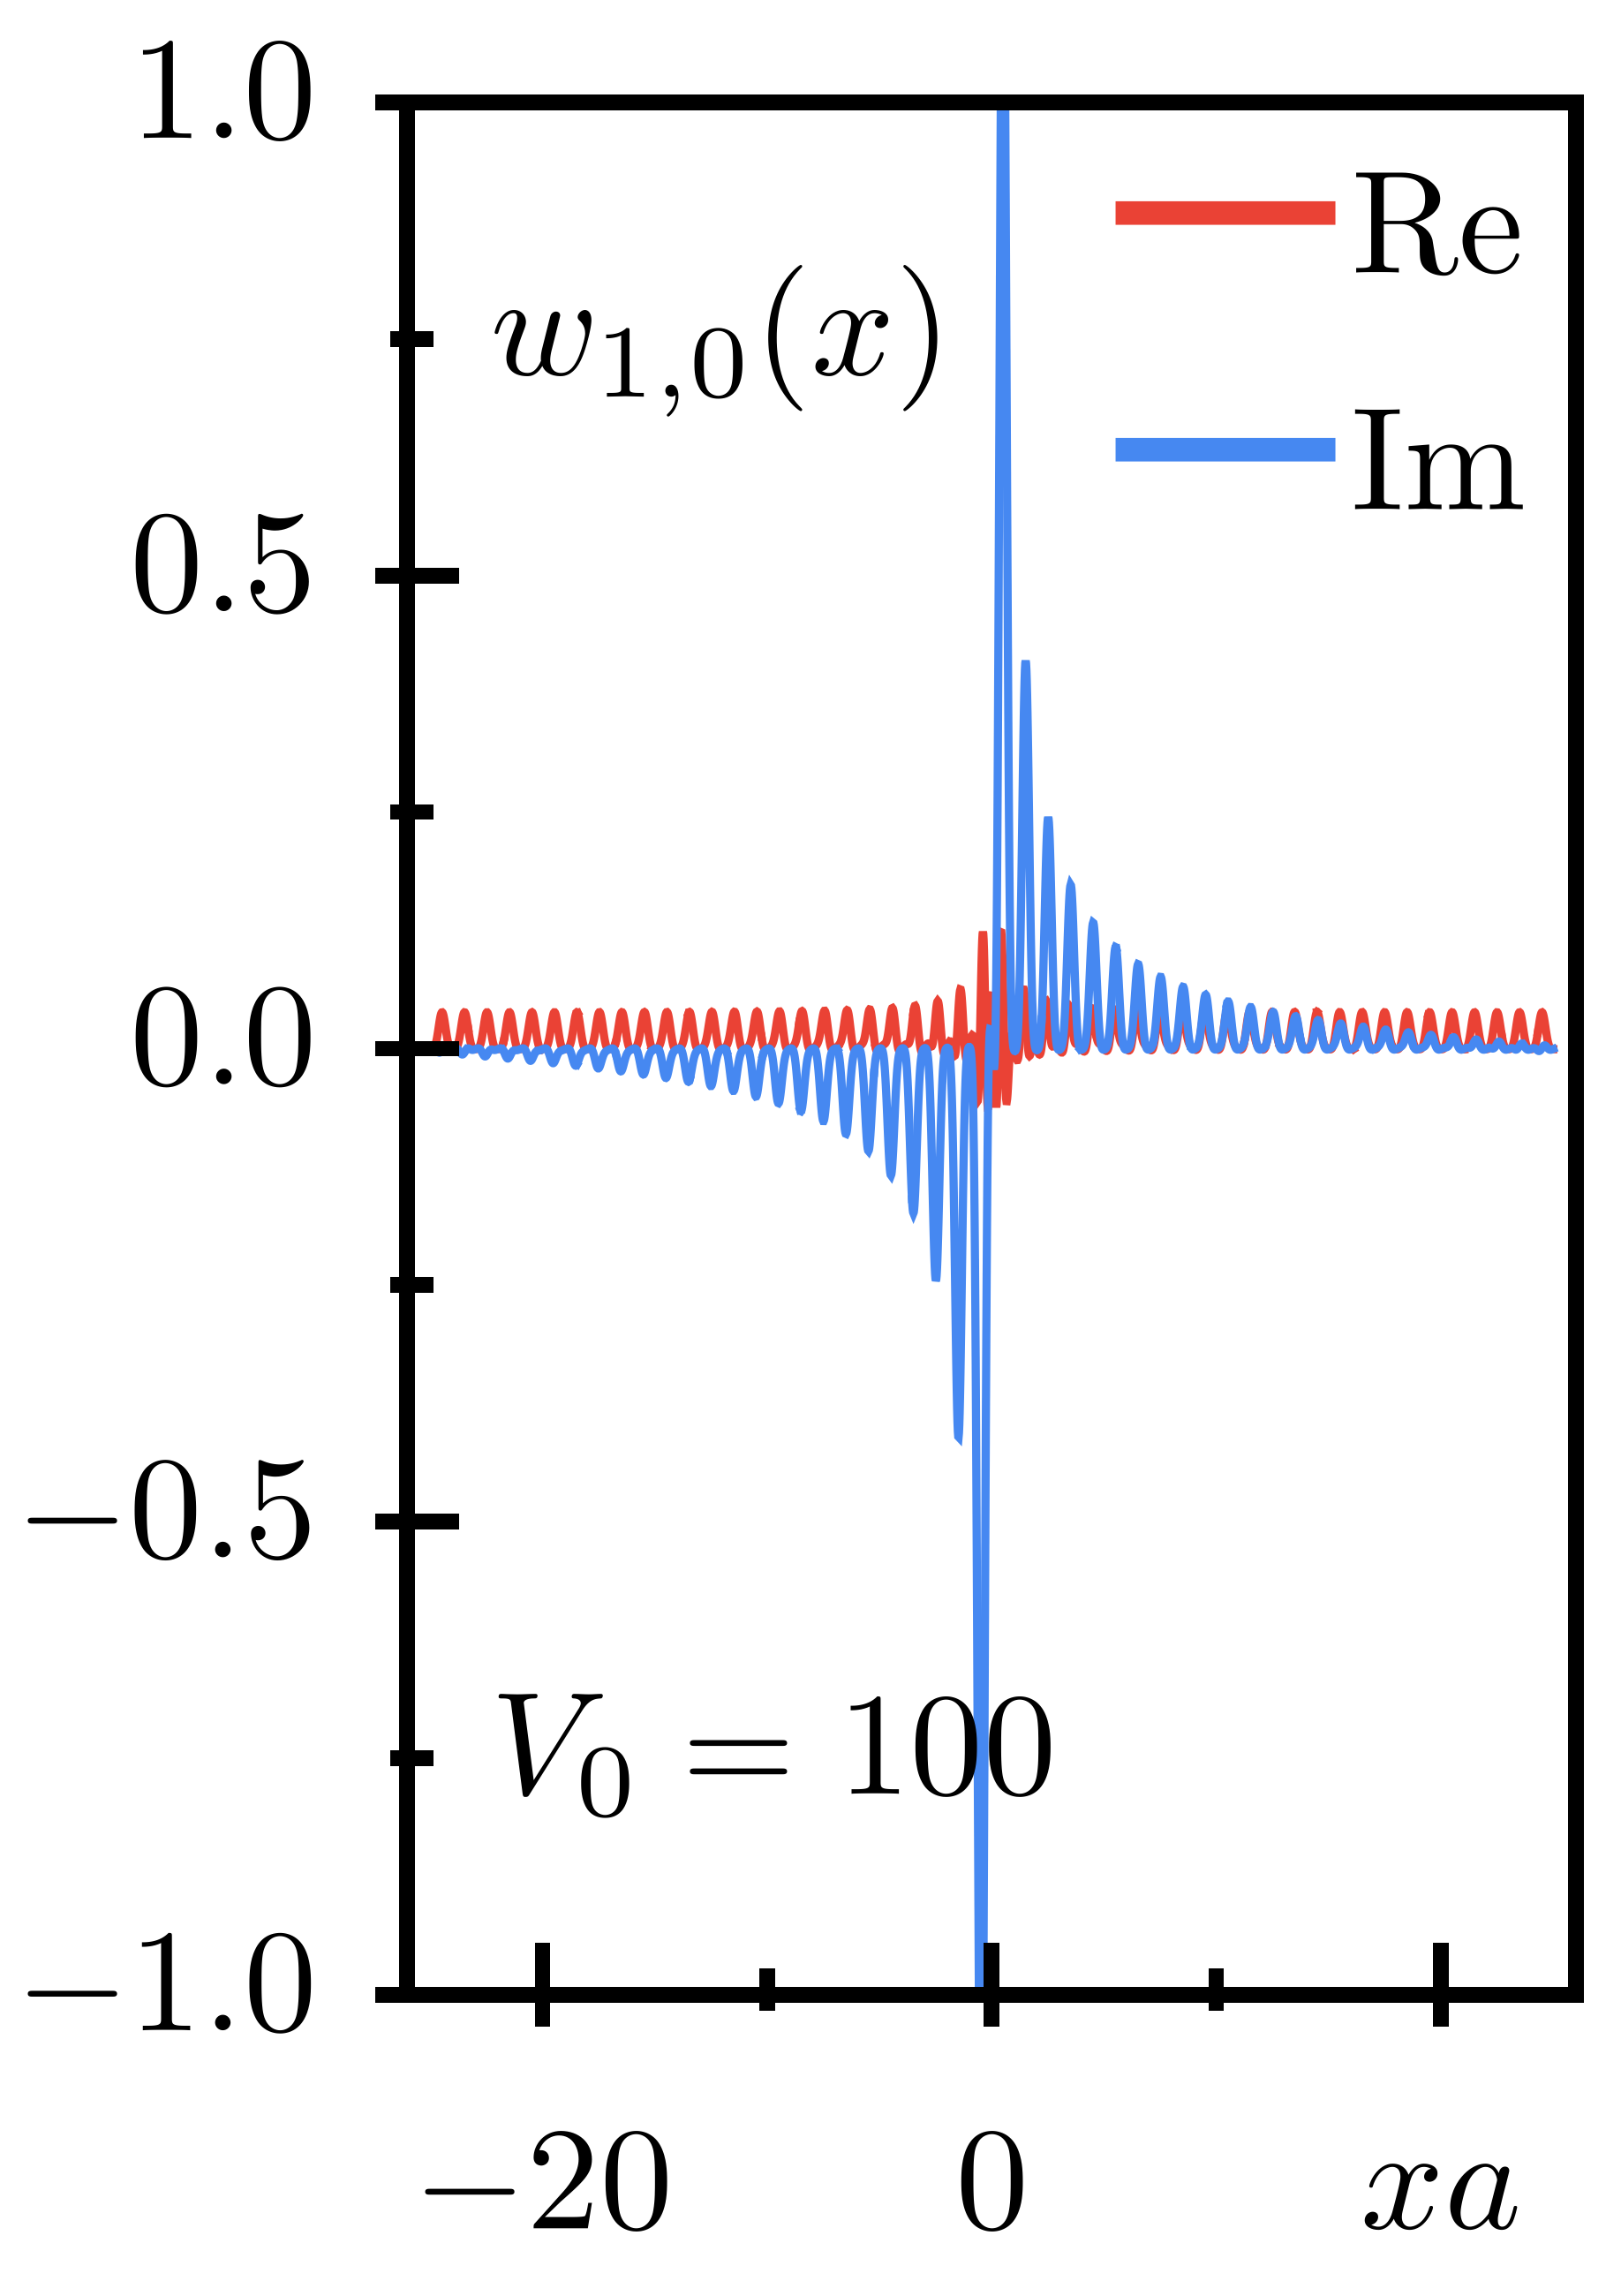
\includegraphics{figures/wannier1_100.png}}\\
    \subfigure[]{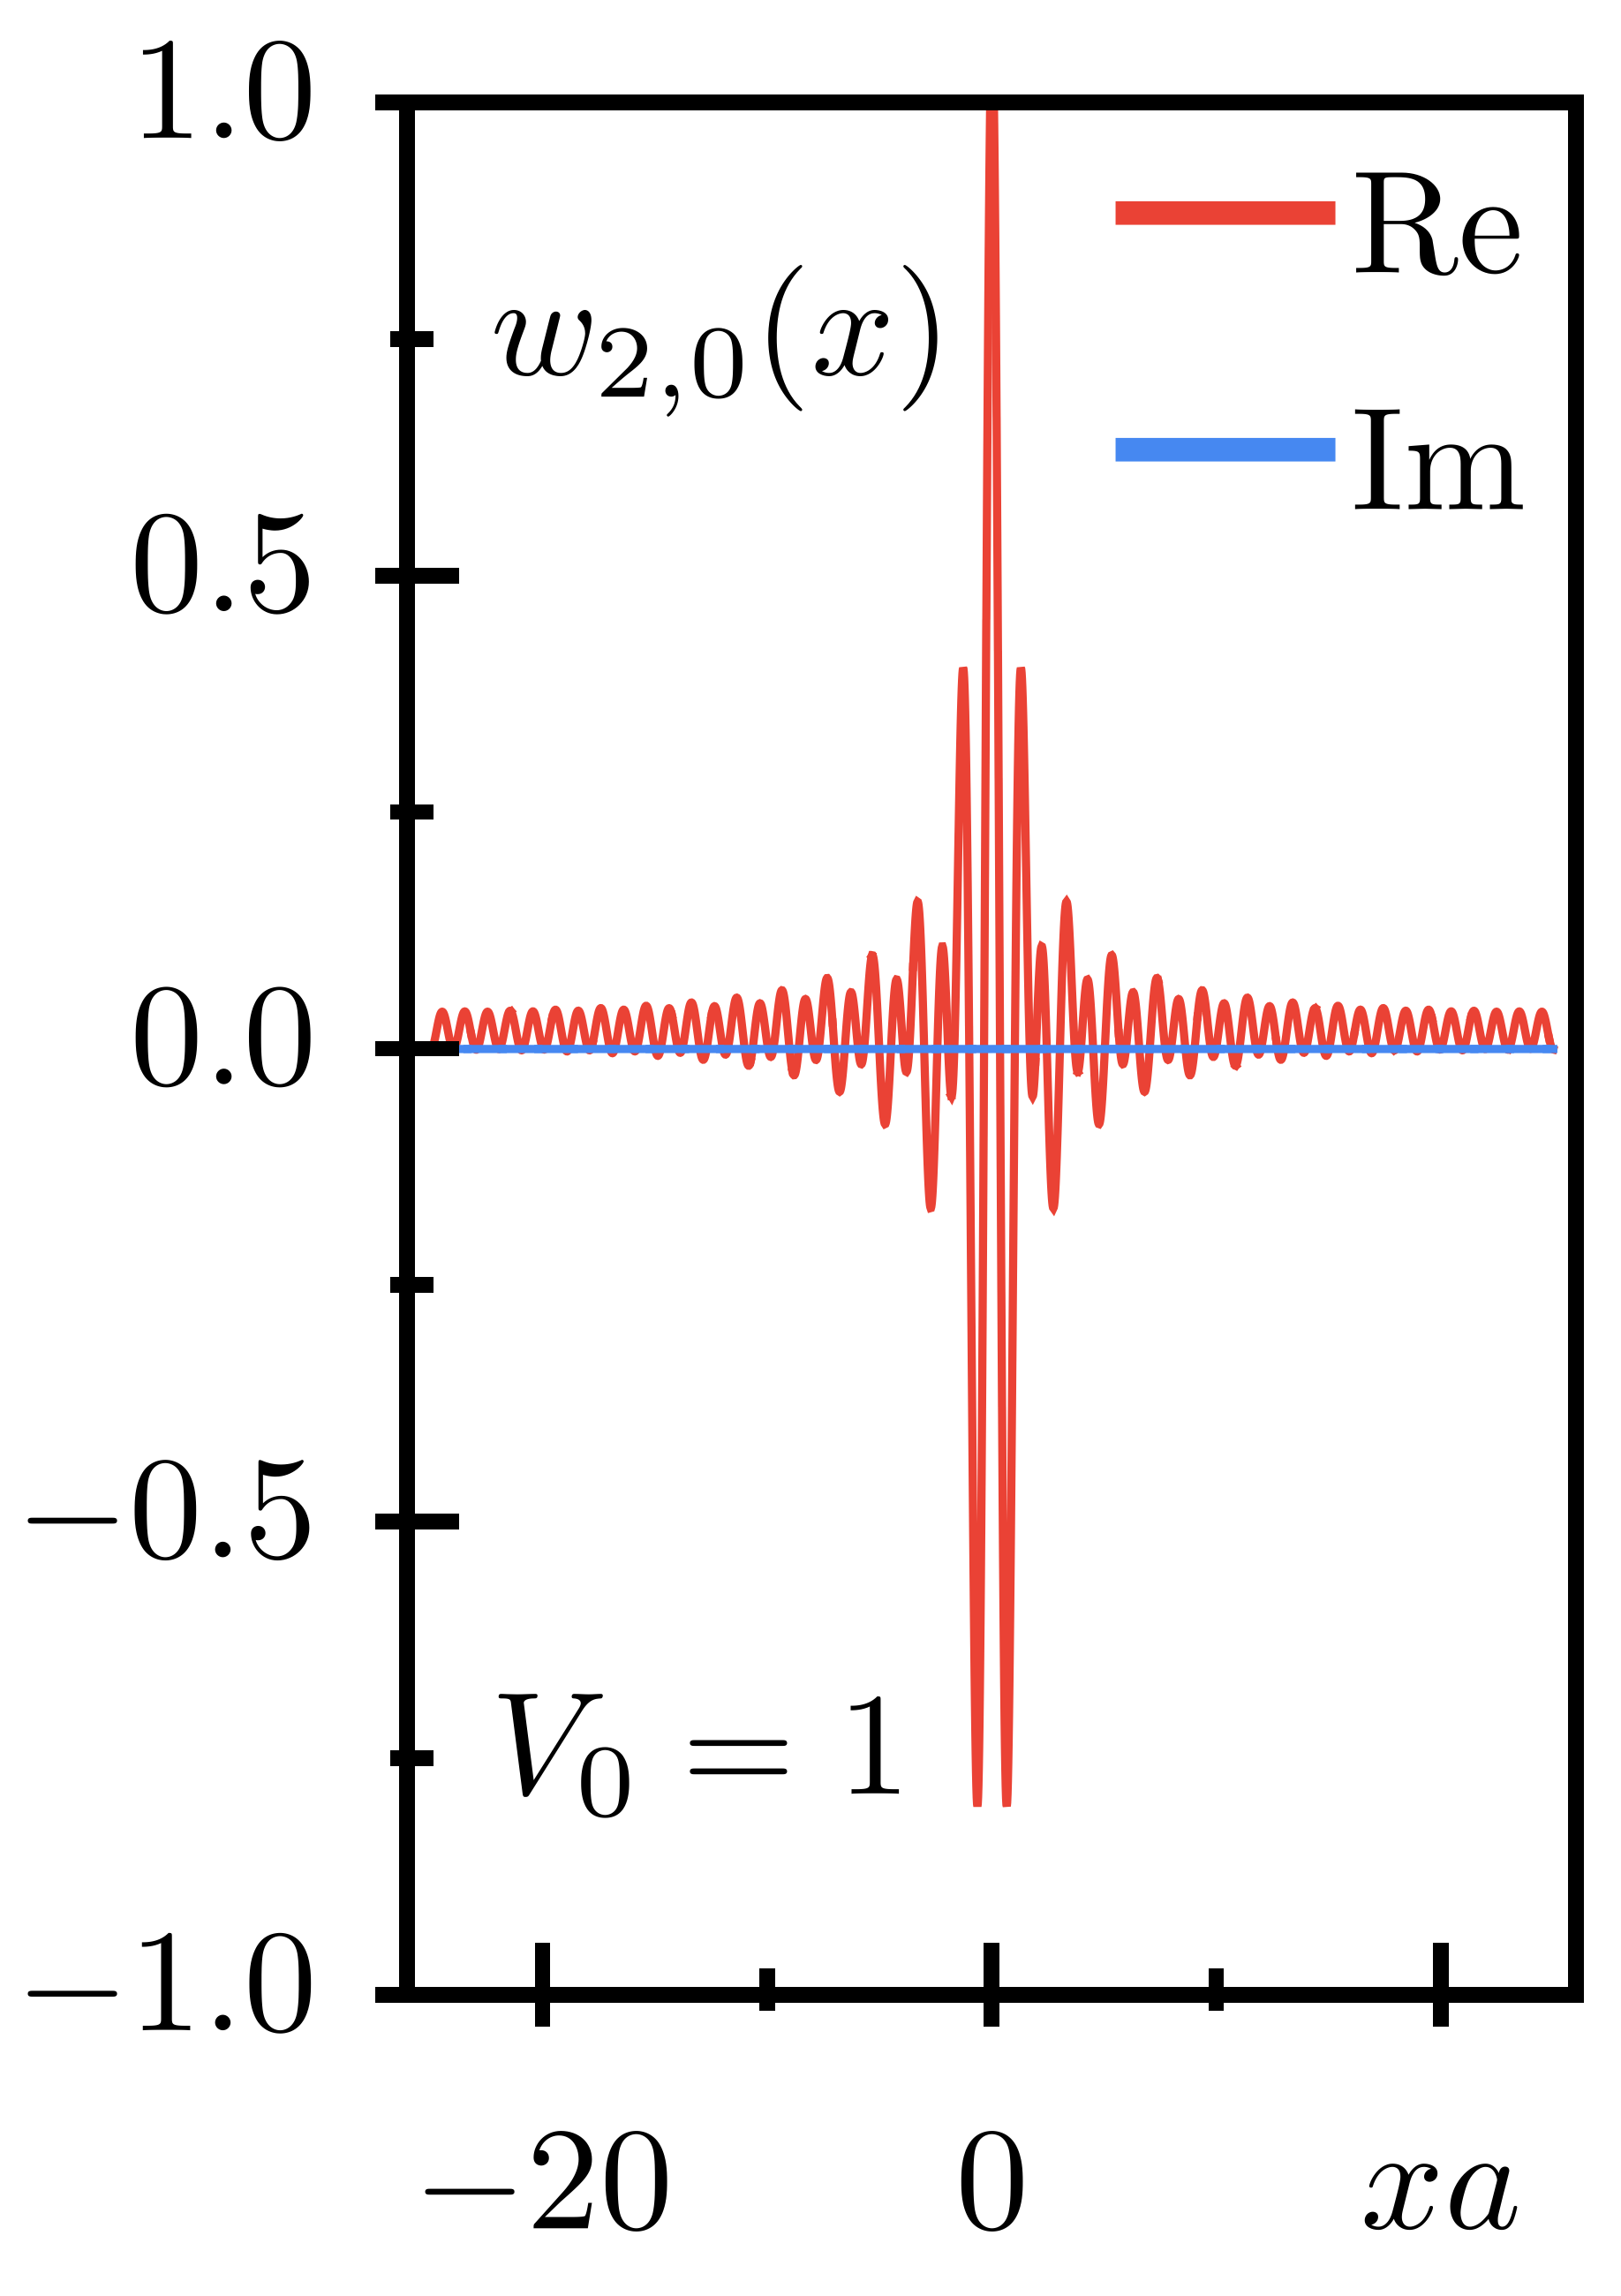
\includegraphics{figures/wannier2_1.png}}
    \subfigure[]{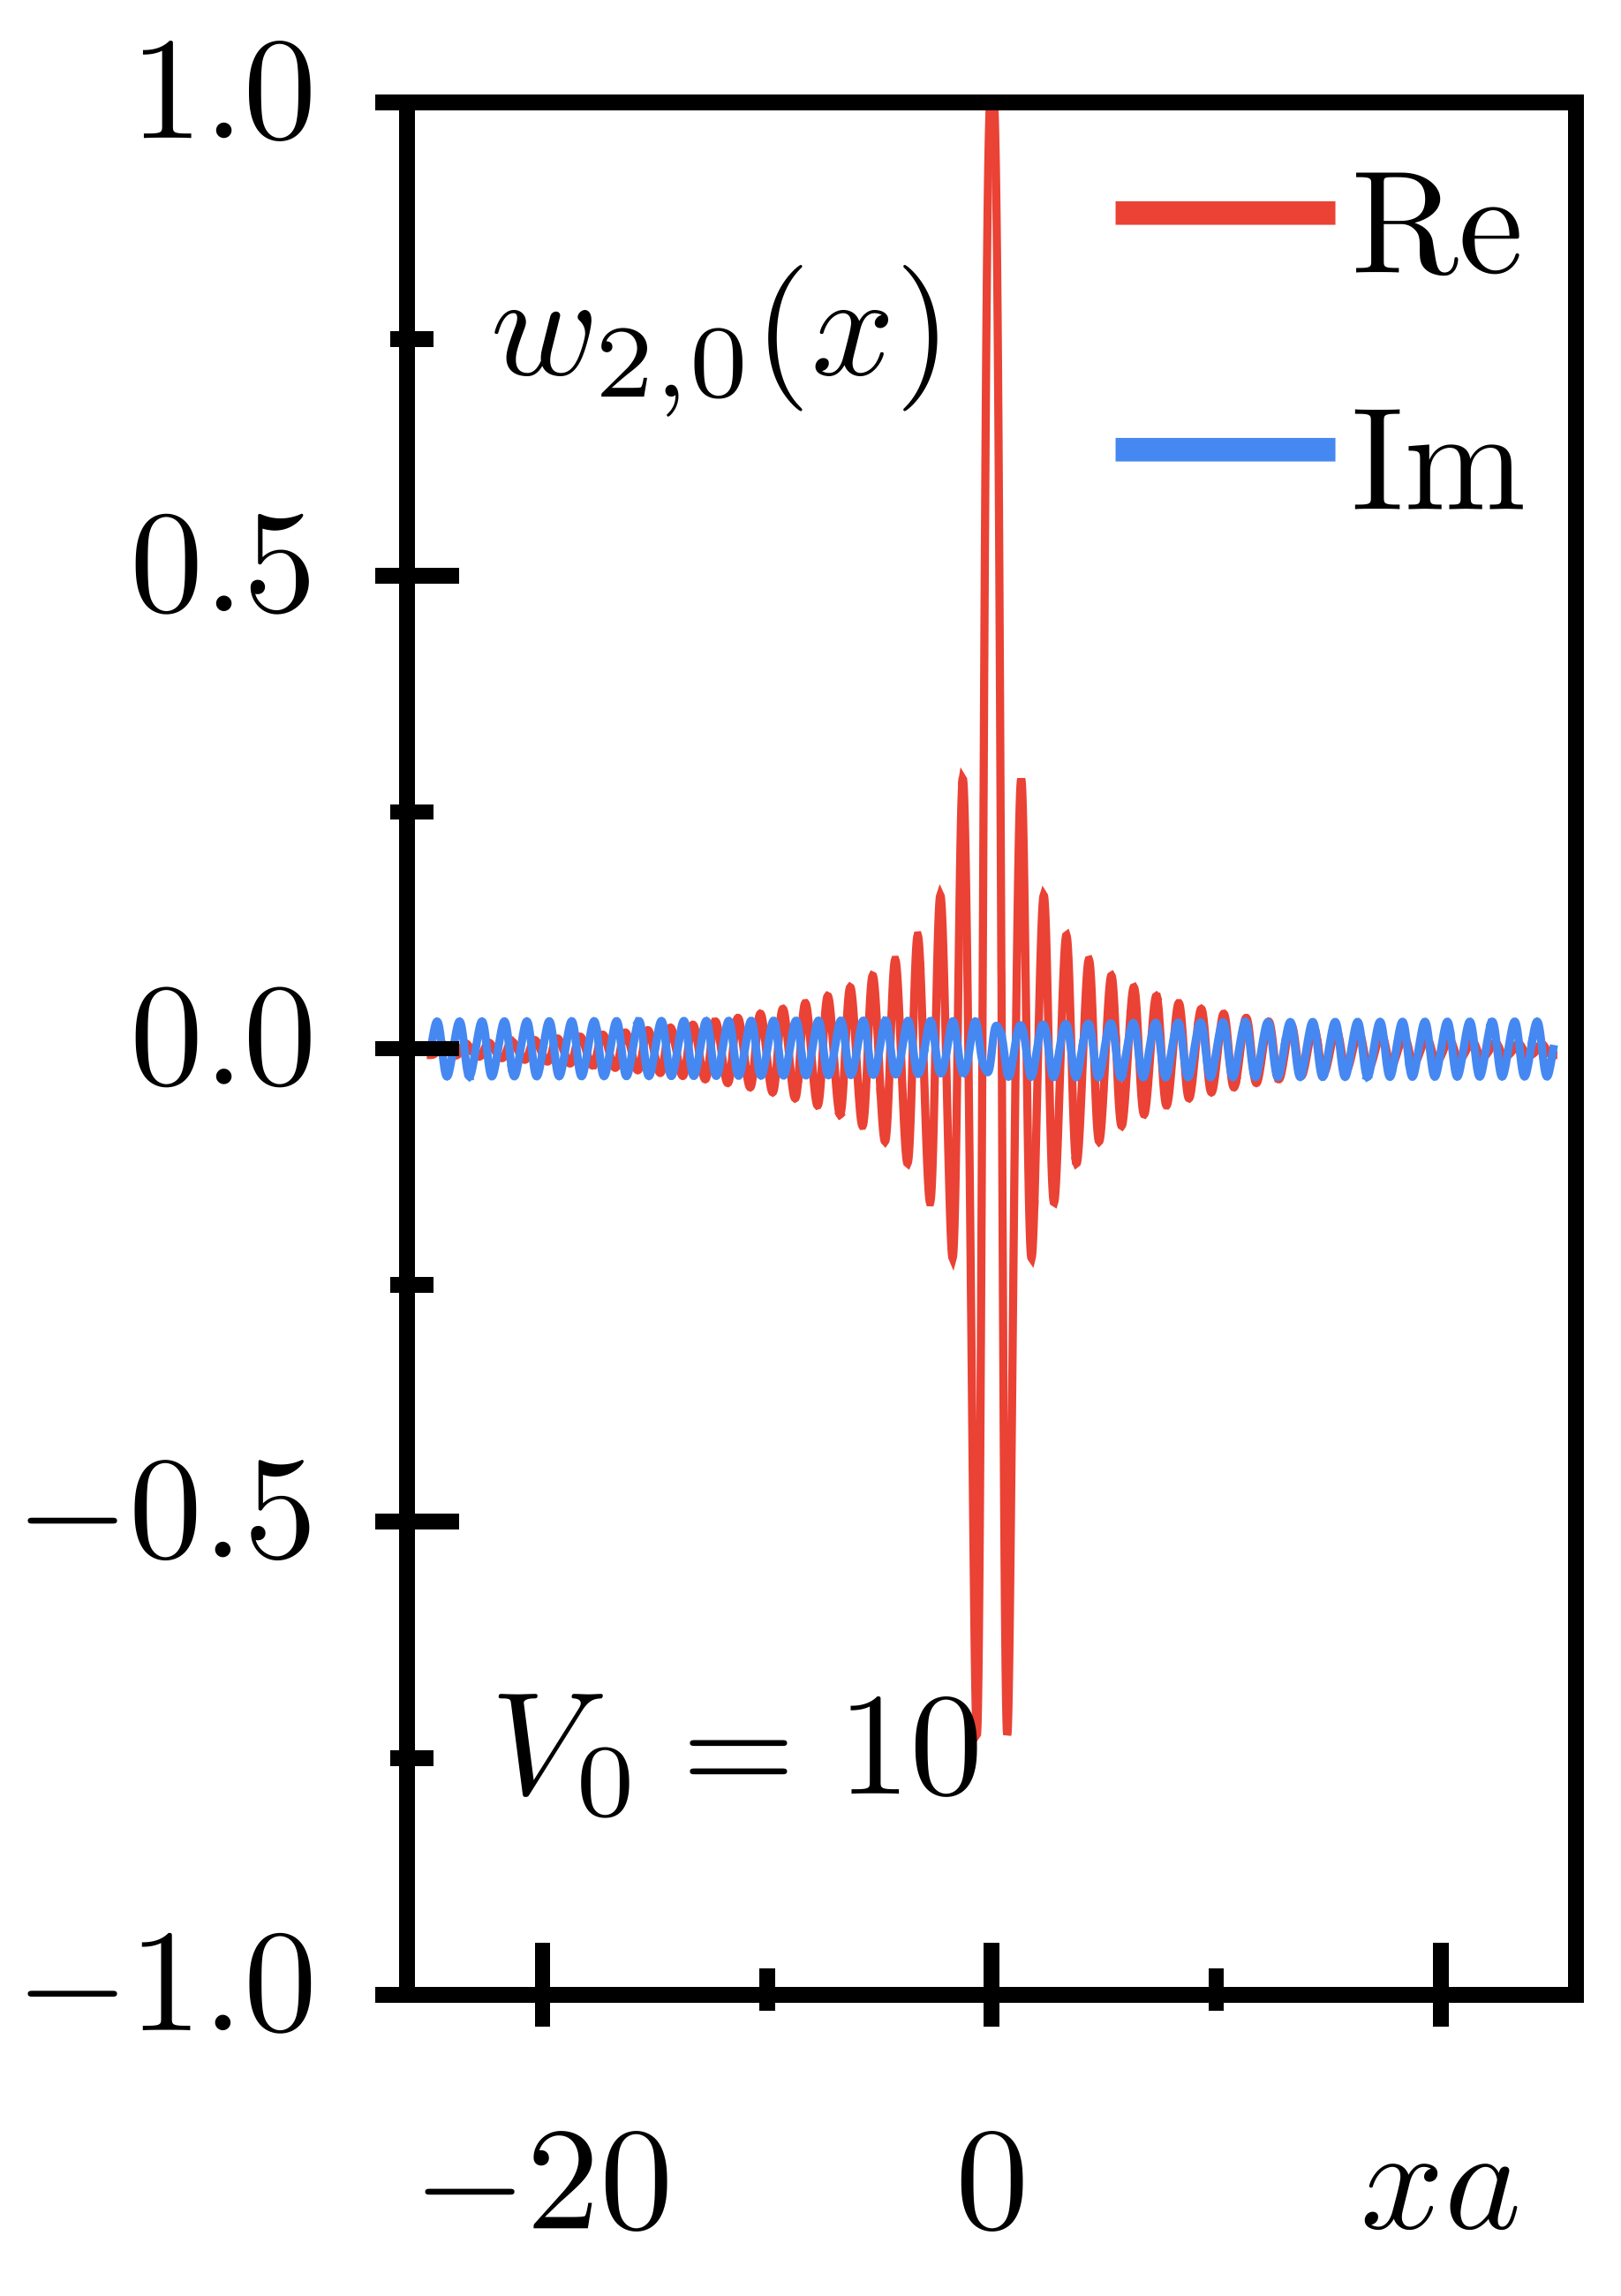
\includegraphics{figures/wannier2_10.png}}
    \subfigure[]{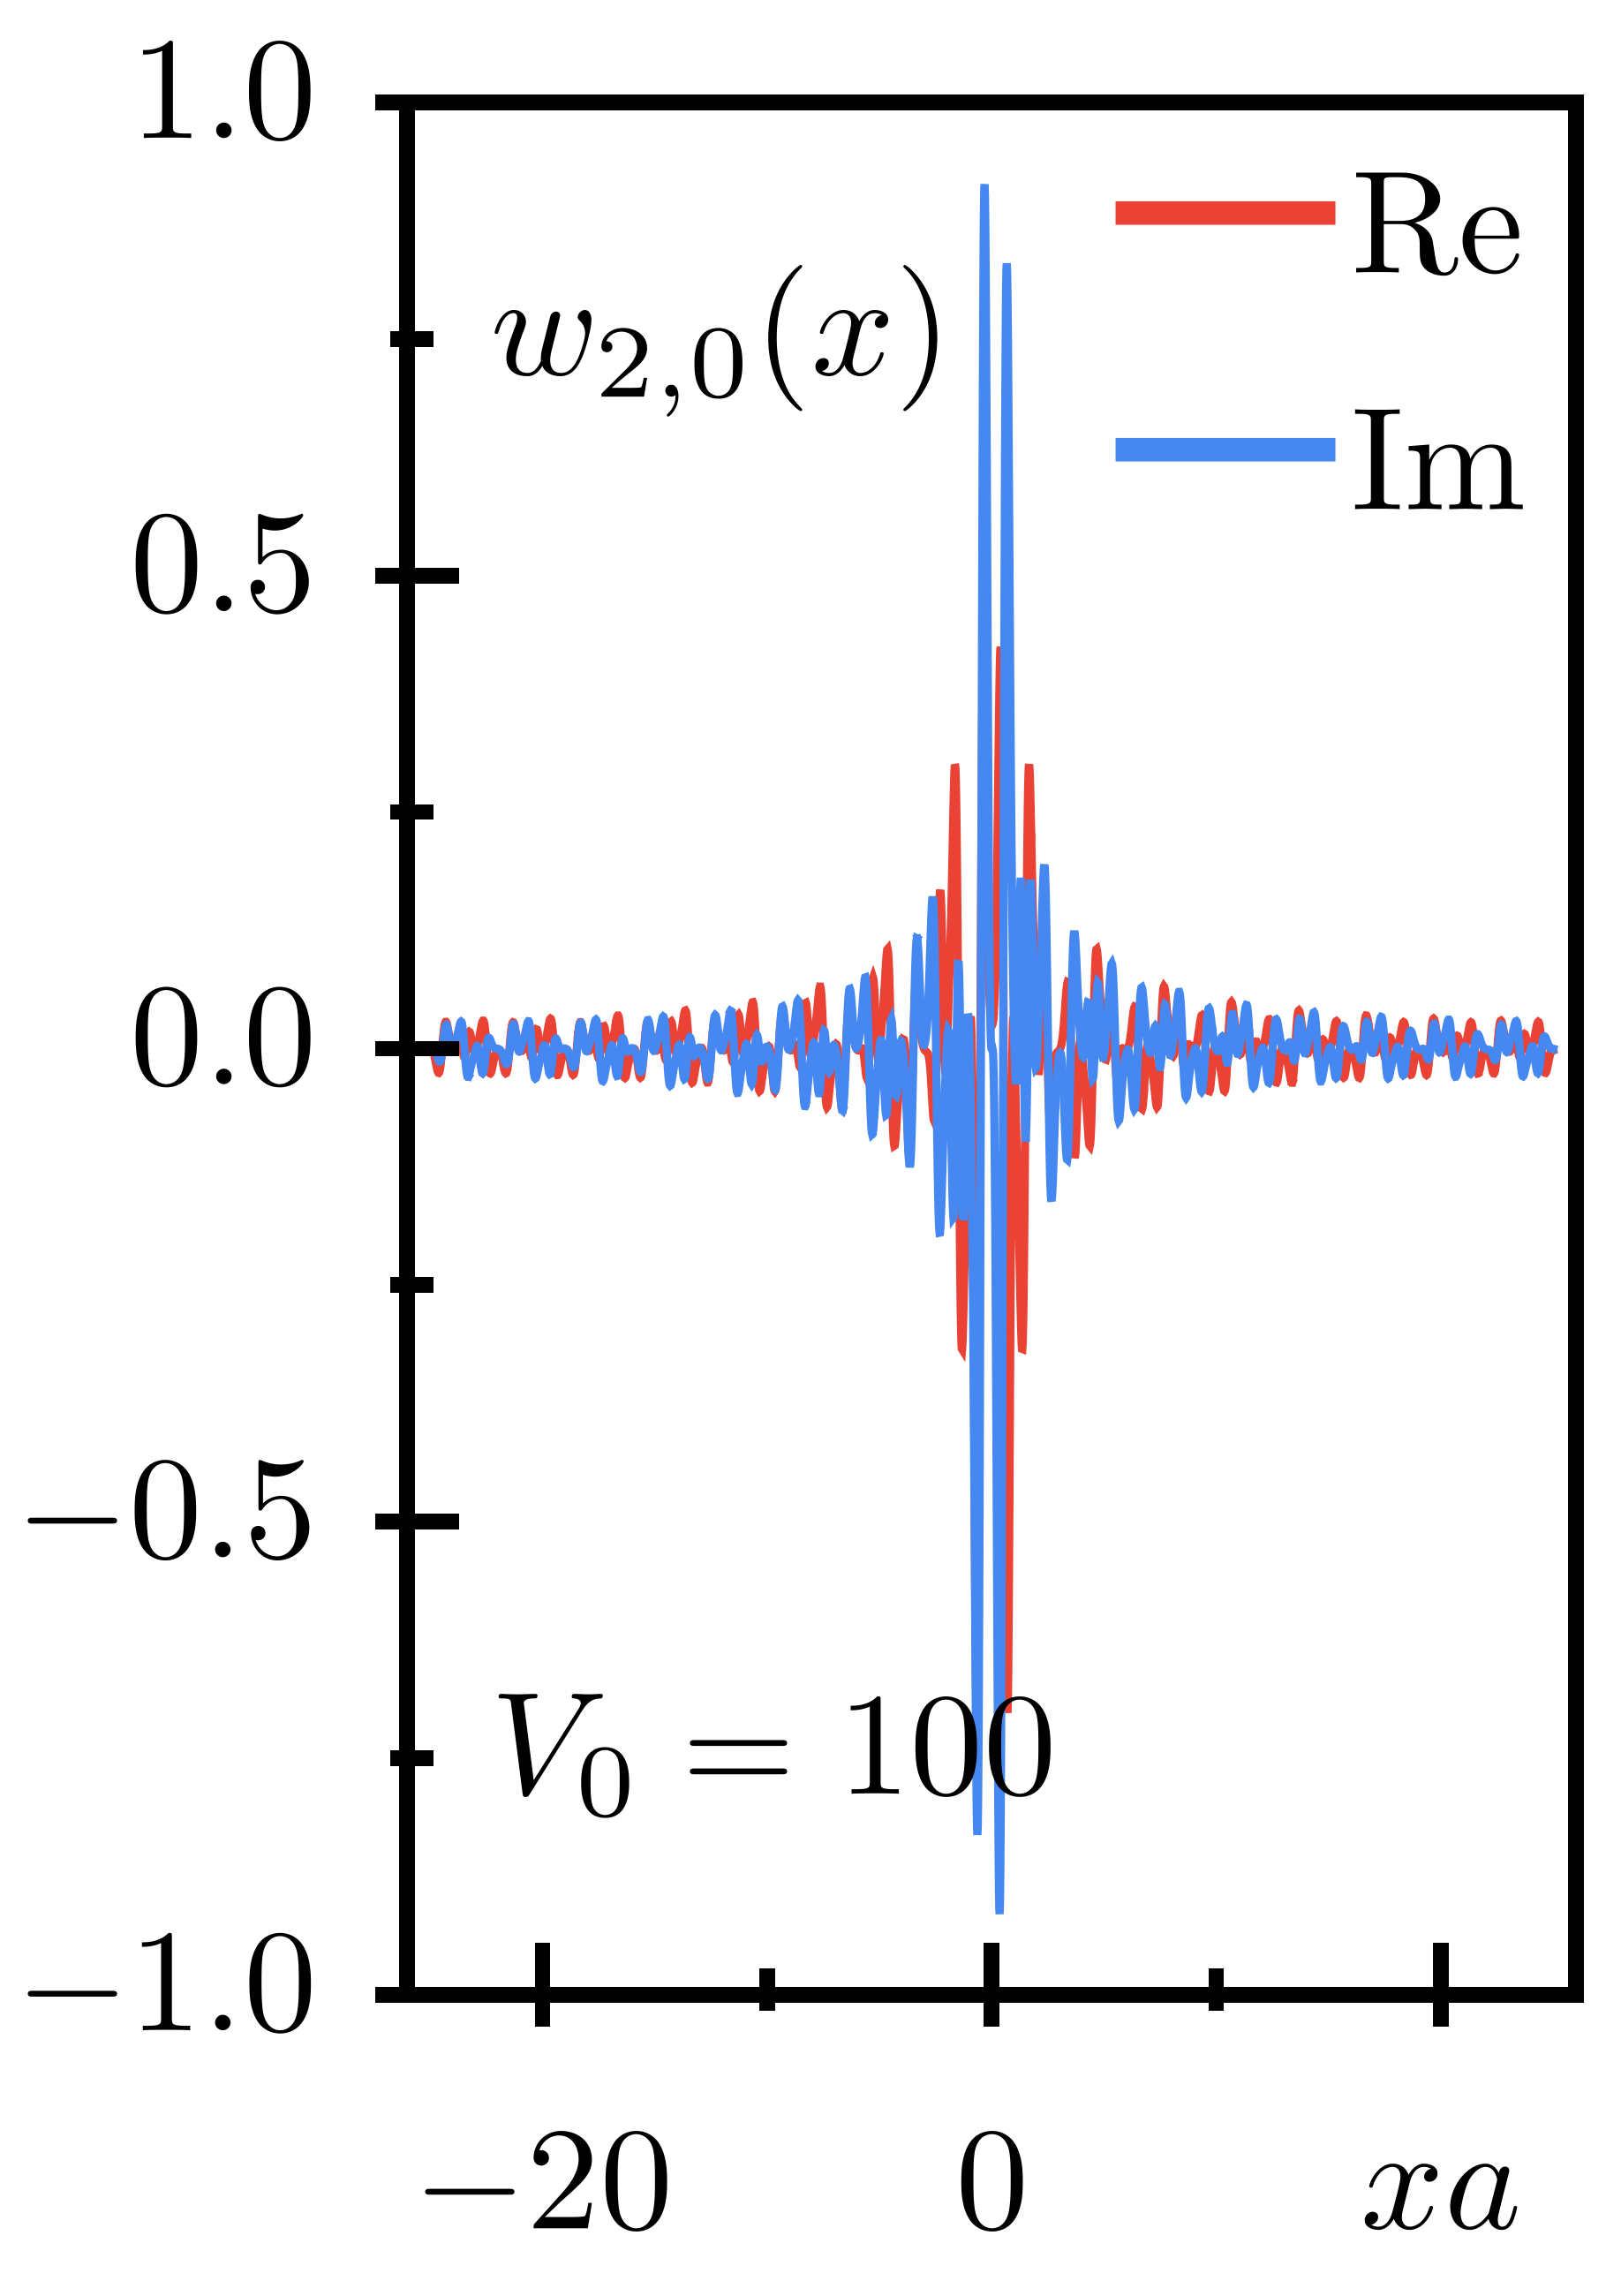
\includegraphics{figures/wannier2_100.png}}\\
    \caption{Example Wannier functions of the first two bands for a periodic potential of the form $V_{ae}(x)=V_0\sin(2\pi/ax)$ for different potential depth. The integration of the Bloch states was performed by assuming a periodicity over $L=50$ lattice translations.}
    \label{fig:tight_binding_wanniers}
\end{figure}

For this purpose, we assume the problem of the single-particle Hamiltonian $\hat H_0$ to be fully solved, such that the Bloch states $\psi_{\alpha{\bf k}}$ are determined, diagonalize $\hat H_0$ and have energy eigenvalues $\varepsilon_{\alpha{\bf k}}$.
This allows to introduce the Wannier basis -- a localized basis composed of the Bloch states and defined as
\begin{align}
    \ket{w_{\alpha{\bf R}}} = \frac1{\sqrt N}\sum_{\bf k}\re^{-\ri{\bf k}{\bf R}}\ket{\psi_{\alpha{\bf k}}}.
    \label{eq:wannier_states}
\end{align}
Note that every momentum-resolved Bloch function can be multiplied with a complex phase without changing its properties.
This naturally provides a gauge freedom to optimize the Wannier function's properties -- for instance, the construction of a maximally localized basis~\cite{Marzari2012}.
Without going into details of optimizing Wannier functions, I want to present a basic visualization of these localized states.
For this purpose, let us consider a cosine periodic potential
\begin{align}
    V_{ae}(x) = V_0\cos\brlr{\frac{2\pi}a x}
\end{align}
which yield a particular easy (a tridiagonal Toeplitz) matrix equation for the Bloch vectors presented in \cref{eq:periodic_lattices_numerics}.
To obtain the Wannier functions, we gauge every Bloch function to be purely real at $x=0$, resulting in the examples displayed in \cref{fig:tight_binding_wanniers}.
\\

The existence of localized Wannier states is translated to the language of second quantization by the notion that transformations between a Bloch and Wannier basis is always unitary.
Hence, annihilation and creation operators of Wannier and Bloch states are set in relation by
\begin{align}
    a^\dag_{\alpha{\bf R}s} = \frac1{\sqrt N}\sum_{\bf k}\re^{-\ri{\bf k}{\bf R}}a^\dag_{\alpha{\bf k}s},
    \quad
    a^\dag_{\alpha{\bf k}s} = \frac1{\sqrt N}\sum_{\bf R}\re^{+\ri{\bf k}{\bf R}}a^\dag_{\alpha{\bf R}s}.
    \label{eq:wannier_states_2}
\end{align}
Since the non-interacting Hamiltonian is diagonal in the Bloch basis, the Bloch basis are eigenfunctions with energies $\varepsilon_{\alpha{\bf k}} = \int\rd^dr\, \psi_{\alpha{\bf k}}^* \hat H_0 \psi_{\alpha{\bf k}}$.
In particular, the Hamiltonian is readily cast into the localized basis according to
\begin{align}
    \hat H_0
    =
    \sum_{{\bf k},s}\varepsilon_{\alpha{\bf k}}a^\dag_{\alpha{\bf k}s}a^\pdag_{\alpha{\bf k}s}
    \overset{\text{\cref{eq:wannier_states_2}}}{=}
    \frac1N\sum_{\bf R, R', k}
    \re^{\ri{\bf k}\brlr{{\bf R}-{\bf R'}}}
    \varepsilon_{\alpha{\bf k}}
    a^\dag_{\alpha{\bf R}s}a^\pdag_{\alpha{\bf R'}s}
    =
    \sum_{i, j}T_{\alpha,i,j}
    a^\dag_{\alpha{\bf R}_is}a^\pdag_{\alpha{\bf R}_js}.
    \label{eq:tight_binding_hamiltonian}
\end{align}
The matrix $T_{\alpha}$ contains all amplitudes of transition processes between two lattice centers, to be determined through the dispersion relation of the $\alpha$-band
\begin{align}
    T_{\alpha,i,j} \coloneqq \frac1N\sum_{\bf k}\re^{\ri{\bf k}\brlr{{\bf R}_i-{\bf R}_j}}\varepsilon_{\alpha{\bf k}}.
\end{align}
On an abstract level, the tight binding Hamiltonian denotes quantum particles hopping between lattice sites, connected through the matrix elements $T_{\alpha,i,j}$.
Without quantitative computations of the transition probabilities, we can fix the matrix to $T_{\alpha,i,j}=\sum_rt_{\alpha,r}\delta_{i-r,j} + \hc$ with some constants $t_{\alpha,r}$.
The relation \cref{eq:tight_binding_hamiltonian} has strong implications on the analytic form of the dispersion relation $\varepsilon_{\alpha{\bf k}}$ -- it is fully determined through the geometry of the crystal lattice.
For instance, one-dimensional lattices with single atom unit cells and lattice spacing $a$ have the particularly easy solution
\begin{align}
    \varepsilon_{\alpha k} = \sum_r 2t_r\cos(r ka).
    \label{eq:1D_tight_binding_dispersion}
\end{align}
Note that this equation is consistent with the Kronig-Penney dispersion relation in the tight-binding limit, presented in \cref{eq:kronig_penney_tight_binding_dispersion}.
In higher dimensions, the evaluation of the dispersion relation may become lengthy, but remains always analytic.
\\

In the following chapters, I present results for interacting single-band approximations which allows to fix (and drop) the band index $\alpha$.
This situation is achieved in case the bottom band is sufficiently separated from the second (e.g. through a strong on-site lattice potential).
A corresponding two-body interaction $\hat V_{ee}$ in the single-band approximation reads
\begin{align}
    \hat V_{ee} = \frac12\sum_{i,i',j,j'}\sum_{s,s'}V_{i,i',j,j'}a^\dag_{{\bf R}_is}a^\dag_{{\bf R}_{i'}s'}a^\pdag_{{\bf R}_js'}a^\pdag_{{\bf R}_{j'}s}.
\end{align}
The matrix elements of the interaction are given by the integral expressions
\begin{align}
    V_{i,i',j,j'} = \int\rd^dr\int\rd^dr'\,w^*_{{\bf R}_i}({\bf r})w^*_{{\bf R}_{i'}}({\bf r}')w_{{\bf R}_j}({\bf r}')w_{{\bf R}_{j'}}({\bf r})V_{ee}({\bf r-r'}).
    \label{eq:two_body_interaction_transition_rates}
\end{align}
The explicit determination of the matrix elements requires knowledge of the form of the Wannier states which, for real materials, is an active field of research on its own.
However, these states are localized and as such the transition rate integrals are short-ranged in most cases.
For this reason, it is sufficient to account for transitions and interactions up to nearest neighbors
\begin{align}
    T_{i,j} \approx \mu\delta_{i,j} + t\delta_{i-1,j}+t^*\delta_{i+1,j},
    \quad
    V_{i,i',j,j'} \approx U\delta_{i,j'}\delta_{i',j}\delta_{i,i'} + V\delta_{i,j'}\delta_{i',j}(\delta_{i-1,i'}+\delta_{i+1,i'}).
\end{align}
In summary, we are at liberty to simplify a bit the notation and arrive at the family of Hubbard-type models, written in second quantization
\begin{align}
    \hat H_{\rm Hubbard} = \sum_{i,j,s}t_{i,j}a^\dag_{is}a^\pdag_{js} + \frac U2\sum_{i,s,s'}\hat n_{i,s}\hat n_{i,s'} + V\sum_{i,s,s'}\hat n_{i,s}\hat n_{i+1,s'}.
    \label{eq:hubbard_hamiltonian}
\end{align}
The operator $a_{is}$ annihilates a Wannier state of flavor $s$, localized around the $i$'th lattice position.
Perhaps the most successful description of electrons in solids is band theory -- based on screened many-body interactions described by effective one-body potentials.
This results in a form of \cref{eq:hubbard_hamiltonian} without density-density interactions such that a diagonalization of the hopping matrix $T$ solves the problem.
However, due to its intrinsic single-particle character, band theory cannot reliably capture truly many-body features such as band magnetism or Mott to metal-insulator transitions.
This motivates the study of Hubbard-type models: despite being a brutal simplification of the true two-body interaction, they are the easiest systems that provide an explanation of such interaction-driven features.
Although its apparent innocence, there is no universal treatment of Hubbard models in general.
In one spacial dimension, the Hamiltonian can be solved analytically and thus falls in the category of being ``integrable''~\cite{Essler2005}.
In general, integrability is a quite fragile property and even slight perturbations will break it in general.
The models we study in the next chapters, albeit closely related to the one-dimensional Hubbard model, do not categorize as integrable due to the presence of additional terms that break some of its fundamental symmetries (e.g. the conservation of the particle flavor).
This motivates the use of alternative methods to study the properties of interacting tight binding models.
One of the most prominent and useful analytic concepts in one dimension is the theory of Luttinger liquids (paired with renormalization group theory) which approximates the microscopic model in the low temperature limit.
%
%
%%%%%%%%%%%%%%%%%%%%%%%%%%%%%%
\section{Luttinger liquids}
\label{sec:luttinger_liquids}
%%%%%%%%%%%%%%%%%%%%%%%%%%%%%%
Luttinger liquids provide a viable tool to study the low-temperature properties of many systems in one and two dimensions.
I start by giving a basic overview on the mapping from spinless fermions to particle-hole excitations in the vicinity of the Fermi points before I introduce the more general formulas for spinful models.
\subsection{The Tomonaga Luttinger model}
We are interested to build an effective model in one dimension capturing the relevant degrees of freedom at low temperatures.
With that purpose, let us start by the free fermionic 1D Hamiltonian $\hat H_0$ denoted by the following (diagonal) representation in momentum space
\begin{align}
    \hat H_0 = \sum_k \frac{(\hbar k)^2}{2m}\hat n_k
    \label{eq:hamiltonian_free_particles}
\end{align}
with dispersion relation $\varepsilon_k =\frac{k^2}{2m}$ depicted in \cref{fig:1D_quadratic_dispersion}.
\begin{figure}
    \centering
    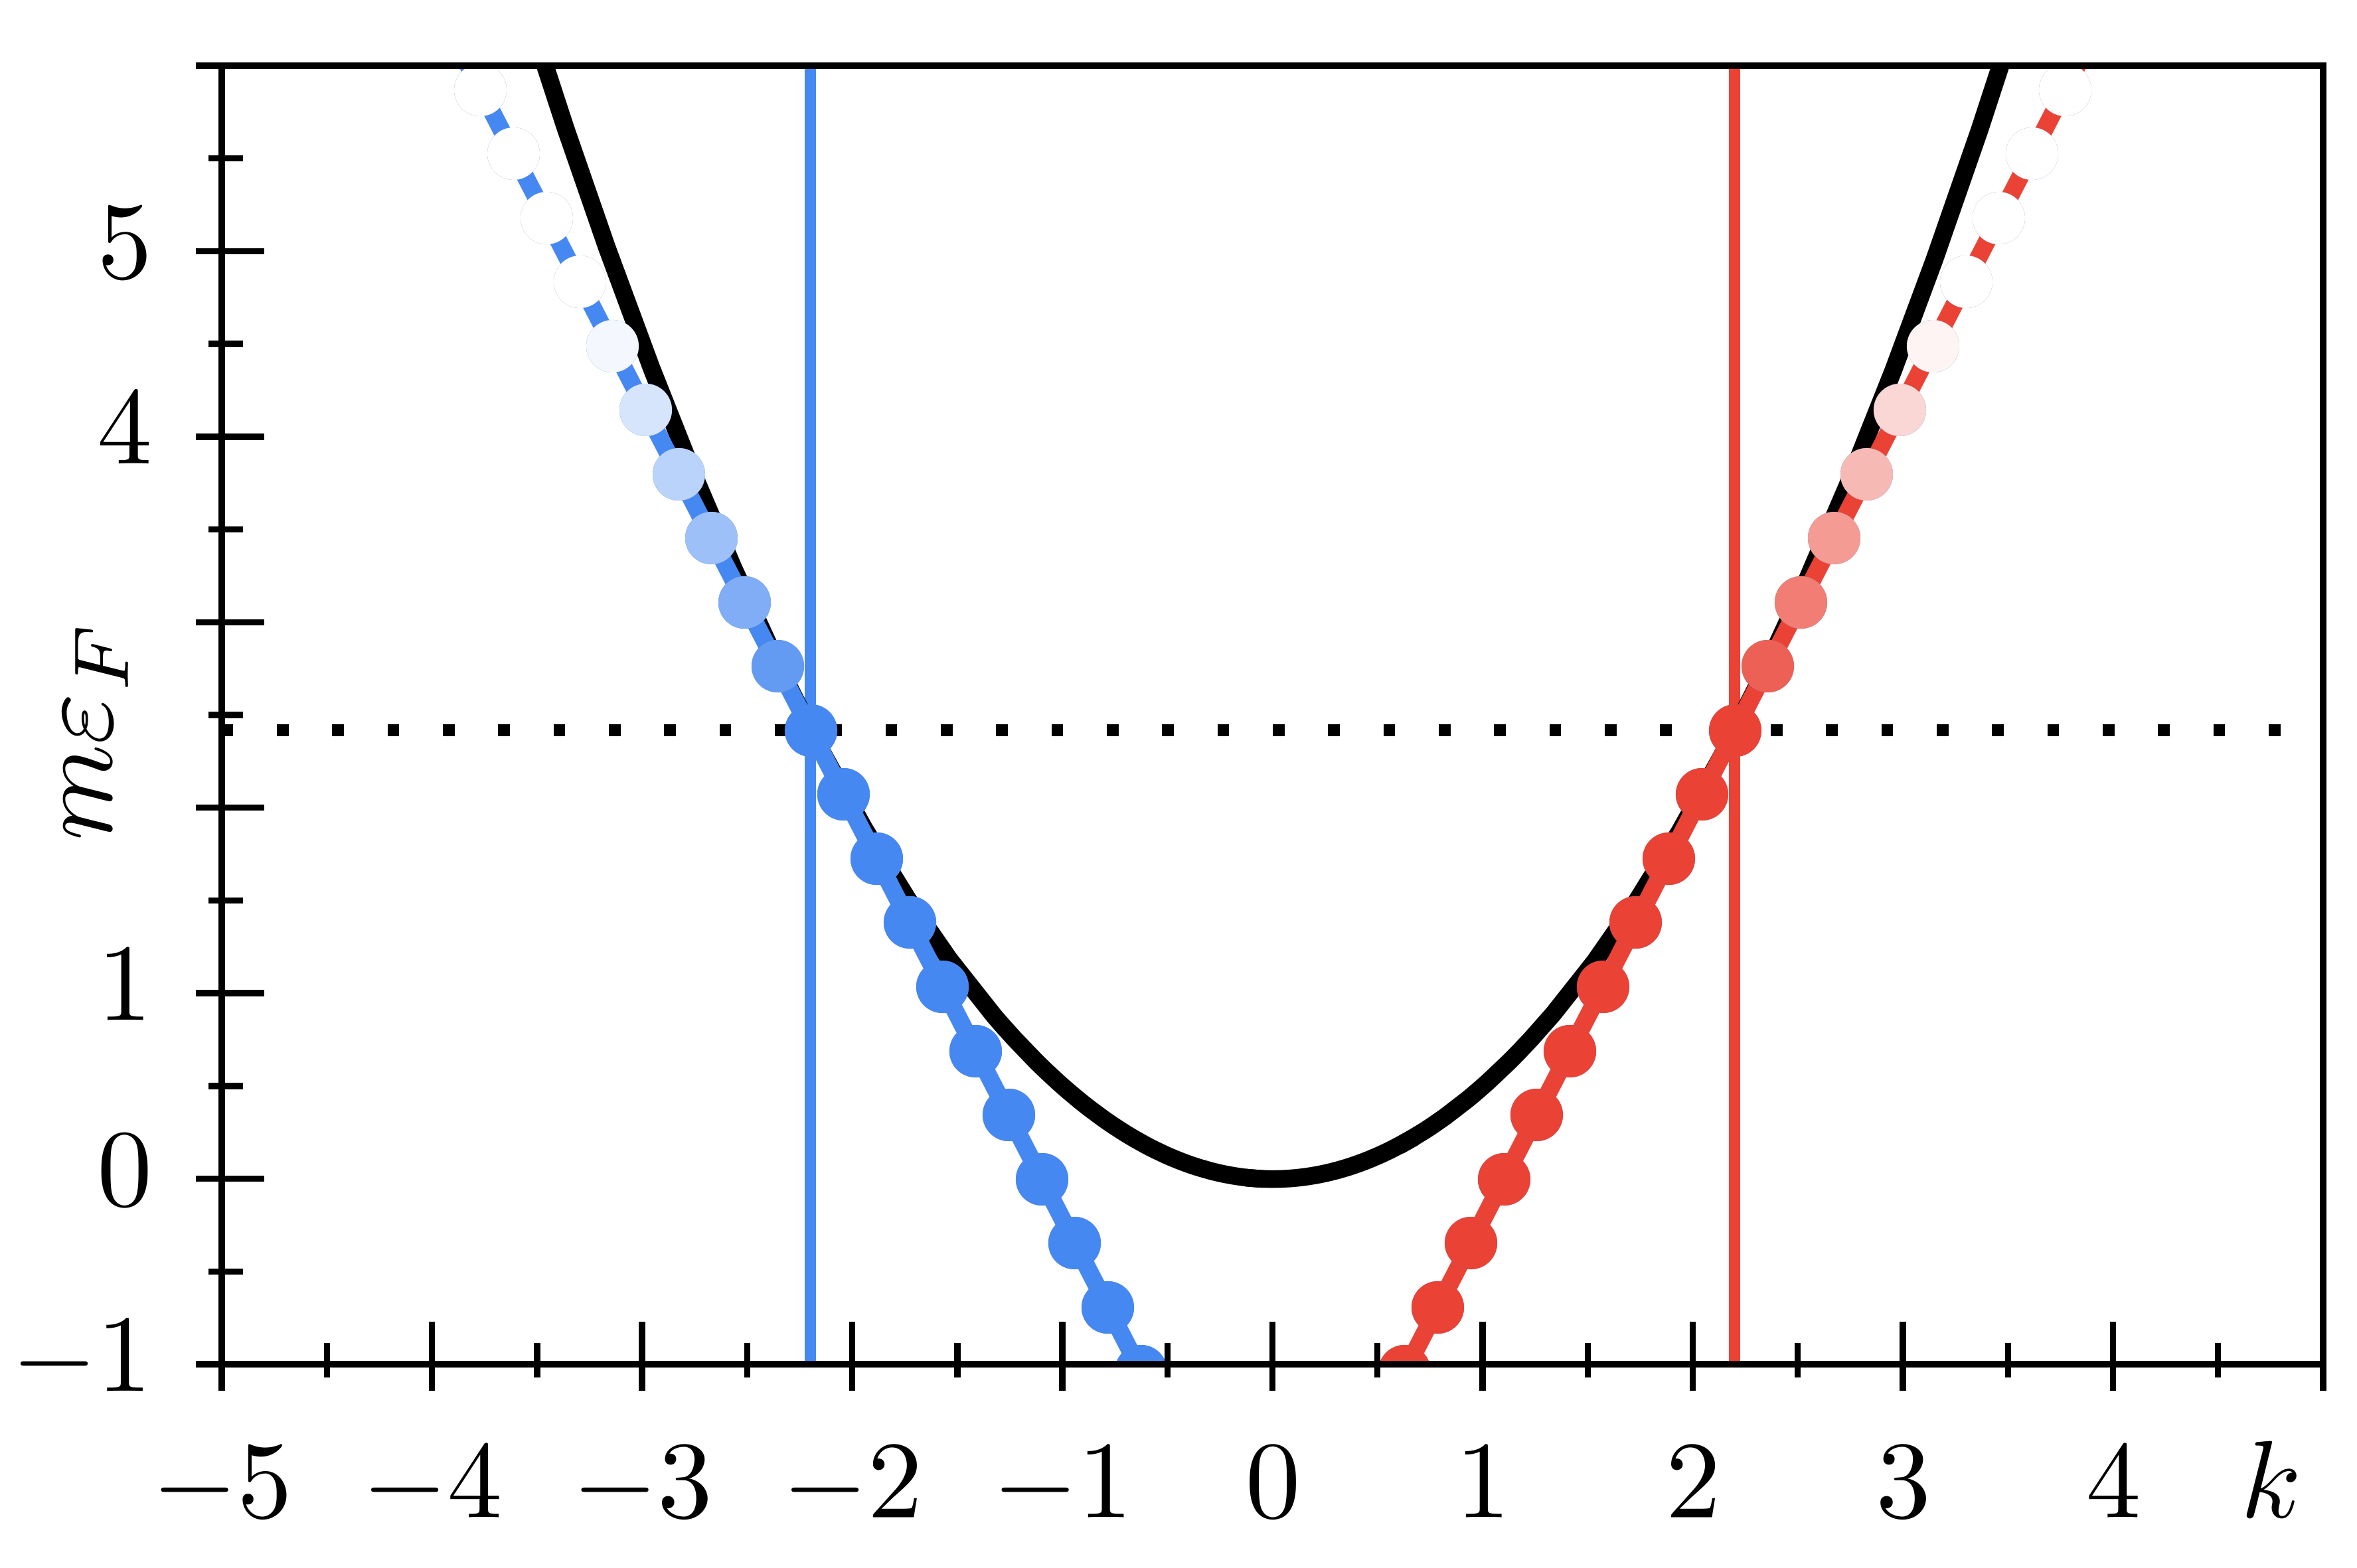
\includegraphics{figures/1D_quadratic_dispersion.png}
    \caption{Quadratic dispersion relation with approximations close to the Fermi energy $\varepsilon_F$.}
    \label{fig:1D_quadratic_dispersion}
\end{figure}
Close to the Fermi energy $\varepsilon_F\coloneqq\varepsilon_{\pm k_F}$, we can approximate the free dispersion and obtain a system of two different species
\begin{align}
    \hat H_0
    &= \sum_k \hbar^2\brlr{\varepsilon_F \pm \frac{k_F}{m}(k\mp k_F) + \mathcal{O}(k^2)}\hat n_k
    \\
    &= \sum_q \hbar^2\brlr{\varepsilon_F + \frac{k_F}{m}q\brlr{\hat n_{q+k_F}-\hat n_{q-k_F}} + \mathcal{O}(k^2)}
    \approx \sum_{q} v_F \hbar q \brlr{c^\dag_{q,R}c^\pdag_{q,R} - c^\dag_{q,L}c^\pdag_{q,L}}
    \label{eq:dispersion_linearization}
\end{align}
which implies a restriction of $q$ to a small window $|q|<\Gamma\ll m\varepsilon_F$ beyond which \cref{eq:dispersion_linearization} is considered to be invalid.
Note the introduction of the so-called right and left operators $c_{R/L,q}$ which annihilate particles propagating to the left/right with Fermi velocity $\pm v_F=\hbar k_F/m$.
\\

For the next part, it will be convenient to understand the meaning of the local density in momentum space, i.e.
\begin{align}
    \hat n(x) = c^\dag_x c^\pdag_x = \frac1L\sum_{k,q}\re^{-\ri x q}c^\dag_{k+q}c^\pdag_{k}.
    \label{eq:local_density}
\end{align}
$\hat n(x)$ thus creates a superposition of particle-hole pairs with characteristic wavelength $q^{-1}$.
The number of particle-hole pairs can be counted through the operator
\begin{align}
    \hat \rho_{-q}\coloneqq \sum_k c^\dag_{k-q}c^\pdag_{k}.
\end{align}
Note further that $\hat\rho_q^\dag = \hat\rho_{-q}$.
By confining the theory close to the Fermi points, there are only two different classes of particle-hole excitations with $q\approx 0$ and $q\approx2k_F$.
The long-wavelength excitations $q\approx0$ are particle-hole pairs of the same species (left or right movers), and excitations of $q\approx2k_F$ are particle-hole pairs of a mixture of the two.
This implies drastic consequences on the relevant action of operators, which we will see in the following.
Let us note here that the density operator of the left/right species $\hat\rho_{\tau,q}$, $\tau\in\{L,R\}$ applied to a Fermi sea creates stable particle-hole excitations (i.e. particles and holes propagate with the same velocity $\pm v_F$) and can thus be used to construct a complete basis of the subspace $\FS^N$ -- for this rather dry discussion, I refer to~\cite{vonDelft1998}.
The consequences of the approximation in \cref{eq:dispersion_linearization} is easily understood in the single-particle operators
\begin{align}
    c^\dag_x = \frac1{\sqrt L}\sum_k \re^{-\ri k x}c^\dag_k \approx \frac1{\sqrt L}\sum_{|q|<\Gamma}\re^{-\ri (q+k_F) x}c^\dag_{R, q} + \re^{-\ri (q-k_F) x}c^\dag_{L, q}
\end{align}
which is then used to find the local density
\begin{align}
    \hat n(x)
    &\approx \frac1L\sum_{q,q'}\brlr{\re^{-\ri (q+k_F) x}c^\dag_{R, q} + \re^{\ri (k_F-q) x}c^\dag_{L, q}}\brlr{\re^{\ri (k_F+q') x}c^\pdag_{R, q'} + \re^{-\ri (k_F-q') x}c^\pdag_{L, q'}},
    \\
    &= \hat \rho_R(x) + \hat \rho_L(x) + \re^{-2\ri k_F}c^\dag_{R}(x)c^\pdag_{L}(x) + \re^{2\ri k_F}c^\dag_{L}(x)c^\pdag_{R}(x).
\end{align}
The first two terms correspond to the $q\approx0$ part of the density, and scattering occurs on the same side of the dispersion relation.
The last two terms scatters right with left movers and transfers particles from one side to the other, which appears at $q\approx2k_F$.
\\

We now turn to an arbitrary two-body interaction of the form~\cref{eq:two_point_interaction} which reads
\begin{align}
    \hat V
    % &= \frac12\int\rd x'\int\rd x V(x'-x)c^\dag(x')c^\dag(x)c^\pdag(x)c^\pdag(x')
    % \\
    &= \frac12\int\rd r\int\rd x V(r)c^\dag(r+x)c^\dag(x)c^\pdag(x)c^\pdag(r+x),
    \\
    &= \frac1{2L^2}\sum_{kk'll'}\int\rd r\int\rd x V(r)\re^{-\ri r(k-l')}\re^{-\ri x(k-l'+k'-l)}c^\dag_kc^\dag_{k'}c^\pdag_lc^\pdag_{l'},
    % \\
    % &= \frac1{2L}\sum_{kk'lq}\int\rd r V(r)\re^{-\ri rq}\delta_{l,k'+q}c^\dag_kc^\dag_{k'}c^\pdag_lc^\pdag_{k-q}
    \\
    &= \frac1{2L}\sum_{kk'q}V(q)c^\dag_kc^\dag_{k'}c^\pdag_{k'+q}c^\pdag_{k-q}
    = \frac1{2L}\sum_{q}V(q)\hat\rho_q\hat\rho^\dag_{q} - \mu.
    \label{eq:two_body_interaction_momentum_space}
\end{align}
The last term is just a constant $\mu = \frac N{2L}\sum_qV(q)$ and can thus be neglected.
By imposing that relevant contributions act close to the Fermi energy involving only momenta in the interval $|k|\in\{k_F\pm\Gamma\}$, we can split the sum in two contributions, one involving scattering processes at small and the other scattering at large momenta
\begin{align}
    \hat V \approx \frac1{2L}\sum_{q\approx0}V(q)\hat\rho_{q}\hat\rho^\dag_{q} + \sum_{q\approx2k_F}V(q)\hat\rho_{q}\hat\rho^\dag_{q}.
\end{align}
For a later study is important to note that the amplitude of the two different $q\approx0$ processes, denoted by $V(q\approx0)$, is equal and independent on the form of the interaction.
A full classification of hypothetical scattering processes is given in~\cref{fig:scattering_processes}.
\begin{figure}
    \centering
    \subfigure[]{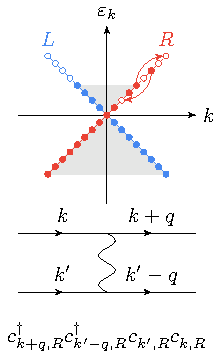
\includegraphics[width=0.328\textwidth]{figures/g4_R.pdf}}
    \subfigure[]{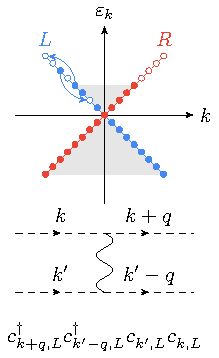
\includegraphics[width=0.328\textwidth]{figures/g4_L.pdf}}
    \subfigure[]{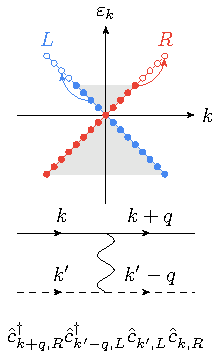
\includegraphics[width=0.328\textwidth]{figures/g2.pdf}}
    \subfigure[]{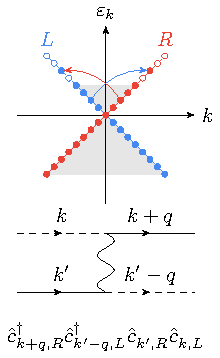
\includegraphics[width=0.328\textwidth]{figures/g1.pdf}}
    \subfigure[]{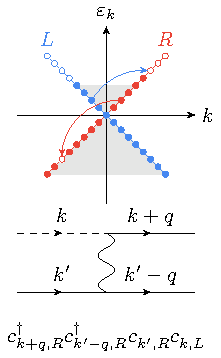
\includegraphics[width=0.328\textwidth]{figures/g13.pdf}}
    \subfigure[]{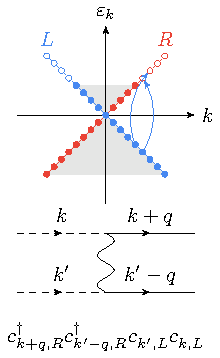
\includegraphics[width=0.328\textwidth]{figures/g22.pdf}}
    \caption{Relevant scattering processes of a generic density-density interaction in one-dimensional quantum systems. (a)/(b) The depicted scattering is commonly referred to as ``forward scattering'' $g_4$ process ($4$ right/left operators, $q\approx0$), (c) as ``backscattering'' $g_2$ process (containing $2$ pairs of right and left operators, $q\approx0$) and (d) as ``Umklapp'' process $g_1$ with momentum transfer $q\approx 2k_F$. Other possible scatterings like the ones depicted in (e) and (f) require the existence of high-energy excitations and are thus exponentially suppressed at low temperatures.}
    \label{fig:scattering_processes}
\end{figure}
This simple argumentation allows to consider only the most relevant processes at low temperatures, i.e. those presented in panels (a) - (d).
We will call those processes forward scattering (note that we are discarding chemical potentials on the right hand side of the following equations)
\begin{align}
    g_4\sum_{k,k',q}c^\dag_{k+q,\tau}c^\dag_{k'-q,\tau}c^\pdag_{k',\tau}c^\pdag_{k,\tau} = g_4 \sum_q\hat\rho^\pdag_{q,\tau}\hat\rho^\dag_{q,\tau},
\end{align}
backscattering
\begin{align}
    g_2\sum_{k,k',q}c^\dag_{k+q,\tau}c^\dag_{k'-q,\overline\tau}c^\pdag_{k',\overline\tau}c^\pdag_{k,\tau} = g_2\sum_q \hat\rho^\pdag_{q,\tau}\hat\rho^\dag_{q,\overline\tau}
\end{align}
and Umklapp scattering
\begin{align}
    g_1\sum_{k,k',q} c^\dag_{k+q,\tau}c^\dag_{k'-q,\overline\tau}c^\pdag_{k',\tau}c^\pdag_{k,\overline\tau}.
\end{align}
I make one important remark on the Umklapp scattering of spinless fermions, that is
\begin{align}
    \sum_{k,k',q}
    c^\dag_{k+q,\tau}c^\dag_{k'-q,\overline\tau}c^\pdag_{k',\tau}c^\pdag_{k,\overline\tau}
    &=
    \sum_{k,k',q,q'} \delta_{q,q'-k+k'}
    c^\dag_{k'+q',\tau}c^\dag_{k-q',\overline\tau}c^\pdag_{k',\tau}c^\pdag_{k,\overline\tau}
    \\
    &=
    -\sum_{k,k',q}c^\dag_{k+q,\tau}c^\dag_{k'-q,\overline\tau}c^\pdag_{k',\overline\tau}c^\pdag_{k,\tau}
    = -\sum_q\hat\rho^\pdag_{q,\tau}\hat\rho^\dag_{q,\overline\tau}.
\end{align}
This proofs that Umklapp terms are up to a sign equivalent to backscattering terms in case of indiscernible particles.
% Umklapp terms cannot be expressed in the density operators of the moving modes $\hat\rho_{q,\tau}$ and, for this reason, are discarded here\footnote{Later, we will see that the Umklapp term in the spinless case are ``marginal'' and can be disregarded under certain conditions.}.
Other processes like those depicted in \cref{fig:scattering_processes} (e) and (f) require the existence of high-energy excitations and can thus be neglected for the effective low temperature theory developed here.
In summary, we can express the interaction in terms of the density-density operators as
\begin{align}
    \hat V \approx \frac{\hbar}{2L}\sum_{q,\tau}\brlr{g_4\hat\rho^\pdag_{q,\tau}\hat\rho^\dag_{q,\tau} + g_2\hat\rho^\pdag_{q,\tau}\hat\rho^\dag_{q,\overline\tau}}
    =
    \frac{\hbar}{L}\sum_{q>0}
    \begin{pmatrix}
        \hat\rho^\pdag_{q,R} & \hat\rho^\pdag_{q,L}
    \end{pmatrix}
    \begin{pmatrix}
        g_4 & g_2 \\
        g_2 & g_4
    \end{pmatrix}
    \begin{pmatrix}
        \hat\rho_{-q,R} \\ \hat\rho_{-q,L}
    \end{pmatrix}
    .
    \label{eq:interaction_densities}
\end{align}
\\

To proceed further, it will be useful to compute the commutation of the density operators
\begin{align}
    \commutator{\hat\rho_{q,\tau},\hat\rho_{q',\tau'}}
    =
    \delta_{\tau,\tau'}\sum_k\brlr{c^\dag_{k+q,\tau}c^\pdag_{k-q',\tau}-c^\dag_{k+q+q',\tau}c^\pdag_{k,\tau}}
    \approx
    -\sigma_\tau\delta_{\tau,\tau'}\delta_{q,-q'}\frac{qL}{2\pi}
    \label{eq:chiral_density_commutation}
\end{align}
in which $\sigma_\tau=\pm1$ for $\tau=R/L$, respectively, and the right hand side is obtained through a projection on the ground state\footnote{This is a reasonable approximation for small interactions only (as a result from a first order perturbative expansion). For a more thorough discussion of \cref{eq:chiral_density_commutation}, see~\cite{Giamarchi2003}.}.
We are now in shape to define canonical bosonic operators representing the interaction degrees of freedom for $q>0$
\begin{align}
    b^\dag_{+q} \coloneqq \sqrt\frac{2\pi}{qL}\hat\rho_{-q,L},
    \quad
    b^\pdag_{+q} \coloneqq \sqrt\frac{2\pi}{qL}\hat\rho_{+q,L},
    \\
    b^\dag_{-q} \coloneqq \sqrt\frac{2\pi}{qL}\hat\rho_{+q,R},
    \quad
    b^\pdag_{-q} \coloneqq \sqrt\frac{2\pi}{qL}\hat\rho_{-q,R},
    \label{eq:canonical_bosonic_operators}
\end{align}
that satisfy the commutation relation $\commutator{b_q^\pdag,b_{q'}^\dag} = \delta_{q,q'}$.
Using \cref{eq:canonical_bosonic_operators} results in a familiar expression for the interaction written in \cref{eq:interaction_densities}, i.e.
\begin{align}
    \hat V \approx\sum_{q>0}\frac{\hbar q}{2\pi}
    \begin{pmatrix}
        b_q & b^\dag_{-q}
    \end{pmatrix}
    \begin{pmatrix}
        g_4 & g_2 \\
        g_2 & g_4
    \end{pmatrix}
    \begin{pmatrix}
        b^\dag_q \\ b_{-q}
    \end{pmatrix}
    .
    \label{eq:quadratic_interactions}
\end{align}
The interaction, originally quartic in the fermionic degrees of freedom, can be cast into a (quadratic) sum of bosonic operators which are the low-energy excitations of the original model.
All that is left to do is to cast the kinetic term into this new basis, which is actually a quite lengthy calculation if we were to approach it by brute-force.
There is an indirect reasoning through Schur's lemma: if two operators $\hat H$ and $\hat H'$ have identical commutation relations with all $\{c^\pdag_\alpha,c^\dag_\alpha\}$, then the two operators are equal up to a chemical potential.
One can easily verify the commutator of the mover-density with the kinetic Hamiltonian
\begin{align}
    \commutator{\hat H_0, \hat\rho_{q,\tau}}
    =
    \sum_{p,\tau'}v_F\sigma_{\tau'}\hbar \commutator{\hat n_{p,\tau'},\hat\rho_{q,\tau}}
    =
    \sigma_\tau v_F \hbar q \hat\rho_{q,\tau}
\end{align}
and find its equivalent expression in bosonic degrees of freedom to be
\begin{align}
    \hat H_0' = \frac{\hbar \pi v_F}L\sum_{q,\tau}\hat\rho_{q,\tau}\hat\rho_{-q,\tau} = \frac{2\hbar\pi v_F}L\sum_{q>0,\tau}\hat\rho_{q,\tau}\hat\rho_{-q,\tau},
\end{align}
which can be verified through evaluation of
\begin{align}
    \commutator{\hat H_0',\hat\rho_{q,\tau}}
    \overset{\text{\cref{eq:recursive_commutation}}}{=}
    -\frac{\hbar \pi v_F}L
    \sum_{p,\tau'}
    \brlr{
    \commutator{\hat\rho_{q,\tau},\hat\rho_{p,\tau'}}\hat\rho_{-p,\tau'}
    -
    \hat\rho_{p,\tau'}\commutator{\hat\rho_{q,\tau},\hat\rho_{-p,\tau'}}
    }
    =
    \sigma_\tau v_F \hbar q\hat\rho_{q,\tau}
\end{align}
and thus we conclude our previous statement $\hat H_0' = \hat H_0 + \mu$ with an irrelevant constant $\mu$.
The effective low energy Hamiltonian containing kinetic and interaction energy satisfies the following matrix equation
\begin{align}
    \hat H = \hat H_0 + \hat V \approx
    \sum_{q>0}\frac{\hbar q}{2\pi}
    \begin{pmatrix}
        b_q & b^\dag_{-q}
    \end{pmatrix}
    \begin{pmatrix}
        2\pi v_F + g_4 & g_2 \\
        g_2 & 2\pi v_F + g_4
    \end{pmatrix}
    \begin{pmatrix}
        b^\dag_q \\ b_{-q}
    \end{pmatrix}
    .
    \label{eq:luttinger_hamiltonian_nondiagonal}
\end{align}
As a final step, we want to find the spectrum of the previous Hamiltonian through a basis transformation $B_q = T B'_q$\footnote{The matrix coupling the dot product of the operator spinors $B_q$ is independent on the momentum $q$ and as such the basis transformation $T$ will not depend on $q$ as well.} with $B_q = (b_q^\dag, b_{-q})^T$ such that
\begin{align}
    \hat H = \sum_{q>0}\hbar qB^\dag_q H B^\pdag_q = \sum_{q>0}\hbar qB'^\dag_q T^\dag H T B'^\pdag_q
\end{align}
is in its diagonal form.
Naive (unitary) rotations do not preserve the commutators of the spinor $B$, defined through
\begin{align}
    \commutator{B_{q,i}^\pdag,B^\dag_{q,j}} = \commutator{B_{q,i}'^\pdag,B'^\dag_{q,j}} = (-\sigma_z)_{i,j}
\end{align}
which imposes an additional constraint on the transformation $T$ according to
\begin{align}
    T^\dag\sigma_z T = \sigma_z,
    \quad
    T^\dag = \sigma_zT^{-1}\sigma_z.
\end{align}
We thus find the similarity relation between the original and the rotated basis according to
\begin{align}
    H'=T^\dag HT =\sigma_z T^{-1}\sigma_z H T,
\end{align}
which allows us to solve the eigenvalue equation of $\sigma_z H$ without knowing the explicit form of $T$.
Since $\sigma_zH$ has vanishing trace, its spectrum is symmetric $\pm E$ and we arrive at the appealing result $H' = u\mathbb1$ with the $2\times2$ unit matrix $\mathbb1$ and scalar eigenvalue
\begin{align}
    u = \frac1{2\pi}\sqrt{\brlr{2\pi v_F + g_4}^2 - g_2^2}
\end{align}
leading to the identity
\begin{align}
    \hat H = \sum_{q>0} u\hbar q B'^\dag_q B'^\pdag_q = \sum_{q>0} \hbar \omega_q B'^\dag_q B'^\pdag_q = \sum_q \hbar  \omega_q b'^\dag_qb'^\pdag_q.
\end{align}
Notice that we succeeded to rewrite the original problem to a sum of decoupled Harmonic oscillators with frequencies $\omega_q\coloneqq u|q|$.
In particular, assuming two canonically conjugate fields $\commutator{\phi_{k},\pi_{k'}} = \ri\hbar\delta_{k,k'}$, the following substitution of ladder operators, i.e.
\begin{align}
    b'_q = \sqrt{\frac{mw_q}{2\pi\hbar}}\brlr{\hat\phi_q + \frac{\ri}{mw_q}\hat\pi_{-q}},
    \quad
    b'^\dag_q = \sqrt{\frac{mw_q}{2\pi\hbar}}\brlr{\hat\phi_{-q} - \frac{\ri}{mw_q}\hat\pi_{q}},
\end{align}
brings the diagonalized Hamiltonian to the more traditional form
\begin{align}
    \hat H = \sum_q \frac{\hat\pi_q\hat\pi_{-q}}{2\pi m} + \frac{m\omega_q^2}{2\pi}\hat\phi_q\hat\phi_{-q}
    =
    \int\frac{\rd x}{2\pi}\, \brlr{\hat\pi^2/m + {Da^2}(\partial_x\hat\phi)^2}.
\end{align}
In the above, I introduced an effective spring constant through the velocity and lattice spacing $D=mu^2/a^2$.
In particular, the field $\partial_x\hat\phi$ can be interpreted as the position offset from the quasiparticle's equilibrium position and $\hat\pi$ is its effective momentum.
Moving to dimensionless units (by imposing $\hbar=c=1$ and requiring a unit mass) and rescaling the fields $\hat\phi\rightarrow \frac1{uK}\hat\phi$, $\hat\pi\rightarrow uK\hat\pi$ results in the standard Luttinger liquid Hamiltonian
\begin{align}
    \hat H = \int\frac{\rd x}{2\pi}\, \brlr{uK\hat\pi^2 + \frac uK(\partial_x\hat\phi)^2},
\end{align}
in which the couplings are encoded in the dimensionless Luttinger parameters
\begin{align}
    u = v_F\sqrt{\brlr{1 + y_4}^2 - y_2^2},
    \quad
    K = \sqrt{\frac{1+y_4-y_2}{1+y_4+y_2}},
    \quad
    y_4=g_4/(2\pi v_F),
    \quad
    y_2=g_2/(2\pi v_F).
\end{align}
The expressions of the effective fields (after the particular choice of the rescaling by a factor $uK$) in terms of the local creation and annihilation operators result from a quite involved calculation which is particularly clearly presented in several excellent books on the topic~\cite{Bruus2004,Giamarchi2003,Gogolin2004}.
On an intuitive level (given the demonstrated equivalence to the quantum harmonic oscillator), the relation to the local densities is straightforward:
\begin{align}
    \partial_x\hat\phi(x)=-\pi[\hat\rho_R(x)+\hat\rho_L(x)],
    \quad
    \hat\pi(x)=\partial_x\hat\theta=\pi[\hat\rho_R(x)-\hat\rho_L(x)].
\end{align}
The relation to the annihilation operators (in the continuum) are maybe less obvious
\begin{align}
    c_{R/L}(x) = \frac1{\sqrt{2\pi\alpha}}\eta_{R/L}\re^{\pm\ri k_F x}\re^{\mp\ri\phi(x) + \ri\theta(x)}
\end{align}
in which the operator identity is to be understood in the limit $\alpha\rightarrow0$\footnote{This limit arises from the fact that the fermionic creation operators are only defined in case of a finite momentum cutoff which is controlled by $\alpha$. For a detailed discussion, I refer to~\cite{Bruus2004}.}.
However, we are able to understand it again from a more intuitive viewpoint:
the operators $\eta$ are called Klein factors which are needed to connect the different subspaces $\FS^N$ of fixed particle number $N$.
The factors $\re^{\pm\ri k_Fx}$ are readily obtained from the confinement of the right/left operators at the two Fermi points.
The last exponential can be understood as a (Grassmann) coherent state composed of (right/left dispersing) particle-hole excitations.
\\

\todo{Add paragraph about correlation functions here}
\\

Lastly, I want to stress that the results presented here are actually independent of the original starting point, i.e. \cref{eq:hamiltonian_free_particles}.
The only microscopic parameter entering in the final theory is $v_F$, which can be replaced by arbitrary group velocities evaluated on the Fermi surface $v_F=(\partial_k\varepsilon_k)_{k=k_F}$.
Significant deviations are then expected in case of flat bands (to be more precise, in case of strong interactions comparable with the bandwidth of the kinetic Hamiltonian), in which case all scattering processes of \cref{fig:scattering_processes} have to be accounted for.
On a practical level, the evaluation of all scattering processes is a tough task and regularly neglected in the vast literature on the theoretical research of one-dimensional models, which then leads to expected quantitative deviations.
However, on a qualitative viewpoint, the neglected scatterings (whenever they are irrelevant in a sense of not opening energy gaps) are widely accepted to change only the effective couplings such that physical consequences predicted from the Luttinger liquid theory [like the asymptotic decay of correlation functions] remain valid.

\subsection{Models with spin}
For spinful systems, we must first require that the kinetic Hamiltonian is fully decoupled, i.e.
\begin{align}
    \hat H_0 = \hat H_{0,\uparrow}+\hat H_{0,\downarrow}
    = \frac{2\hbar\pi v_F}L\sum_{q>0,\tau,s\in\{\uparrow,\downarrow\}}\hat\rho^\pdag_{q,\tau,s}\hat\rho^\dag_{q,\tau,s}
\end{align}
which allows to introduce a pair of conjugate fields $(\phi_s,\theta_s)$ for each spin flavor $s$.
The scattering processes $g_4$ and $g_2$ can be generalized in a straightforward manner, and we achieve
\begin{align}
  \hat V \approx
  \sum_{q,\tau,s}
  g_{4\parallel}\hat\rho^\pdag_{q,\tau,s}\hat\rho^\dag_{q,\tau,s}
  +
  g_{4\perp}\hat\rho^\pdag_{q,\tau,s}\hat\rho^\dag_{q,\tau,\overline s}
  +
  g_{2\parallel}\hat\rho^\pdag_{q,\tau,s}\hat\rho^\dag_{q,\overline\tau,s}
  +
  g_{2\perp}\hat\rho^\pdag_{q,\tau,s}\hat\rho^\dag_{q,\overline\tau,\overline s}
\end{align}
To account for the scattering among different spins, it is customary to write the model in terms of a charge and spin degree of freedom, defined as
\begin{align}
    \hat f_+=\frac1{\sqrt2}\brlr{\hat f_\uparrow + \hat f_\downarrow},
    \quad
    \hat f_-=\frac1{\sqrt2}\brlr{\hat f_\uparrow - \hat f_\downarrow}.
\end{align}
This rotation is trivial on the level of the kinetic Hamiltonian and
\begin{align}
    \hat H_0 = \frac{2\hbar\pi v_F}L\sum_{q>0,\tau,s\in\{+,-\}}\hat\rho^\pdag_{q,\tau,s}\hat\rho^\dag_{q,\tau,s}.
\end{align}
Things are different for the forward and backscattering processes $g_{2/4}$.
In the spinful scenario, it is necessary to distinguish between intra-spin and inter-spin scattering, such that
\begin{align}
  \sum_{s\in\{\uparrow,\downarrow\}}
  \brlr{
  g_{4\parallel}\hat\rho^\pdag_{q,\tau,s}\hat\rho^\dag_{q,\tau,s}
  +
  g_{4\perp}\hat\rho^\pdag_{q,\tau,s}\hat\rho^\dag_{q,\tau,\overline s}
  +
  g_{2\parallel}\hat\rho^\pdag_{q,\tau,s}\hat\rho^\dag_{q,\overline\tau,s}
  +
  g_{2\perp}\hat\rho^\pdag_{q,\tau,s}\hat\rho^\dag_{q,\overline\tau,\overline s}
  }
  \\
  =
  \frac12
  \sum_{i\in\{2,4\}}
  \brlr{
  [g_{i\parallel}+g_{i\perp}]\hat\rho^\pdag_{q,\tau,+}\hat\rho^\dag_{q,\tau,+}
  +
  [g_{i\parallel}-g_{i\perp}]\hat\rho^\pdag_{q,\tau,-}\hat\rho^\dag_{q,\tau,-}
  }.
\end{align}
In case of the Umklapp terms, things become a bit more messy.
While the inter-spin Umklapp terms are again equivalent to backscattering terms (up to a sign), the $g_{1\perp}$ term will be
\begin{align}
    g_{1\perp}\sum_{s\in\{\uparrow,\downarrow\}}c^\dag_{L,s}(x)c^\pdag_{R,s}(x)c^\dag_{R,\overline s}(x)c^\dag_{L,\overline s}(x)
    =
    g_{1\perp}\sum_{s\in\{\uparrow,\downarrow\}}\re^{-2\ri\phi_s(x)}\re^{2\ri\phi_{\overline s}(x)}
    =
    \frac{g_{1\perp}}{2\pi^2\alpha^2}\cos(2\sqrt2\phi_-(x))
\end{align}
and therefore, the total Hamiltonian is of the form
\begin{align}
    \hat H = \sum_{s\in\{+,-\}}\int\frac{\rd x}{4\pi}\brlr{u_s K_s\pi_s^2 + \frac{u_s}{K_s}(\partial_x\phi_s)^2} + \int\rd x\frac{2g_{1\perp}}{(2\pi\alpha)^2}\cos(2\sqrt2\phi_-(x))
\end{align}
with coupling constants
\begin{align}
    u_sK_s = v_F(1+y_{4s}-y_{2s}),
    \quad
    \frac{u_s}{K_s} = v_F(1+y_{4s}+y_{2s}),
    \\
    y_{is} = \frac{g_{i\parallel}+sg_{i\perp}}{2\pi v_F},
    \quad
    i\in\{1,2\},
    \quad
    s\in\{+,-\}.
\end{align}
% %
% %
% %%%%%%%%%%%%%%%%%%%%%%%%%%%%%%%%%%%%
% \section{The harmonic oscillator}
% \label{sec:the_harmonic_oscillator}
% %%%%%%%%%%%%%%%%%%%%%%%%%%%%%%%%%%%%
% %
% %
% %%%%%%%%%%%%%%%%%%%%%%%%%%%%%%%%%
% %%%%%%%%%%%%%%%%%%%%%%%%%%%%%%%%%
% \section{Matrix product states}
% \label{sec:matrix_product_states}
% %%%%%%%%%%%%%%%%%%%%%%%%%%%%%%%%%
% %%%%%%%%%%%%%%%%%%%%%%%%%%%%%%%%%
% %
% %
% %%%%%%%%%%%%%%%%%%%%%%%%%%%%%%%%%%
% \subsection{Exact diagonalization}
% \label{sec:exact_diagonalization}
% %%%%%%%%%%%%%%%%%%%%%%%%%%%%%%%%%%
% %
% %
% %%%%%%%%%%%%%%%%%%%%%%%%%%%%%%%%%%
% \subsection{Schmidt decomposition}
% \label{sec:schmidt_decomposition}
% %%%%%%%%%%%%%%%%%%%%%%%%%%%%%%%%%%
% %
% %
% %%%%%%%%%%%%%%%%%%%%%%%%%%%%%%%%%%%%%%%%%%%%
% \subsection{Variational ground state search}
% \label{sec:variational_ground_state_search}
% %%%%%%%%%%%%%%%%%%%%%%%%%%%%%%%%%%%%%%%%%%%%
% %
% %
% %%%%%%%%%%%%%%%%%%%%%%%%%%%
% \subsection{Time evolution}
% \label{sec:time_evolution}
% %%%%%%%%%%%%%%%%%%%%%%%%%%%
% %
% %
% %%%%%%%%%%%%%%%%%%%%%%%%%%%%%%%%%%%%%%%%
% %%%%%%%%%%%%%%%%%%%%%%%%%%%%%%%%%%%%%%%%
% \section{Topological phases of matter}
% \label{sec:topological_phases_of_matter}
% %%%%%%%%%%%%%%%%%%%%%%%%%%%%%%%%%%%%%%%%
% %%%%%%%%%%%%%%%%%%%%%%%%%%%%%%%%%%%%%%%%
% %
% %
% %%%%%%%%%%%%%%%%%%%%%%%%%%%%%%%%%%%%%%%%%%%
% \subsection{The Su-Schrieffer-Heeger chain}
% \label{sec:the_ssh_chain}
% %%%%%%%%%%%%%%%%%%%%%%%%%%%%%%%%%%%%%%%%%%%
% %
% %
% %%%%%%%%%%%%%%%%%%%%%%%%%%%%%%%%%%%%%%%%%%%%%%%%%%%%%%%%%%
% \subsection{Symmetry classification of topological phases}
% \label{sec:symmetry_classification_of_topological_phases}
% %%%%%%%%%%%%%%%%%%%%%%%%%%%%%%%%%%%%%%%%%%%%%%%%%%%%%%%%%%
%%%%%%%%%%%%%%%%%%%%%%%%%%%%%%%%%%%%%%%%%%%%%%%%%%
%%%%%%%%%%%%%%%%%%%%%%%%%%%%%%%%%%%%%%%%%%%%%%%%%%
\chapter{Topological phases of matter}
\label{ch:topological_phases_of_matter}
%%%%%%%%%%%%%%%%%%%%%%%%%%%%%%%%%%%%%%%%%%%%%%%%%%
%%%%%%%%%%%%%%%%%%%%%%%%%%%%%%%%%%%%%%%%%%%%%%%%%%


%!TEX root = thesis.tex
%%%%%%%%%%%%%%%%%%%%%

\begin{partbacktext}
    \part{Results}
    \label{part:results}
\end{partbacktext}

%!TEX root = thesis.tex
%%%%%%%%%%%%%%%%%%%%%

\chapter{Exploring pretopological phases of matter}
\label{ch:Exploring_pretopological_phases_of_matter}
Write intro
\section{Quantum criticality on a chiral ladder}
Write intro
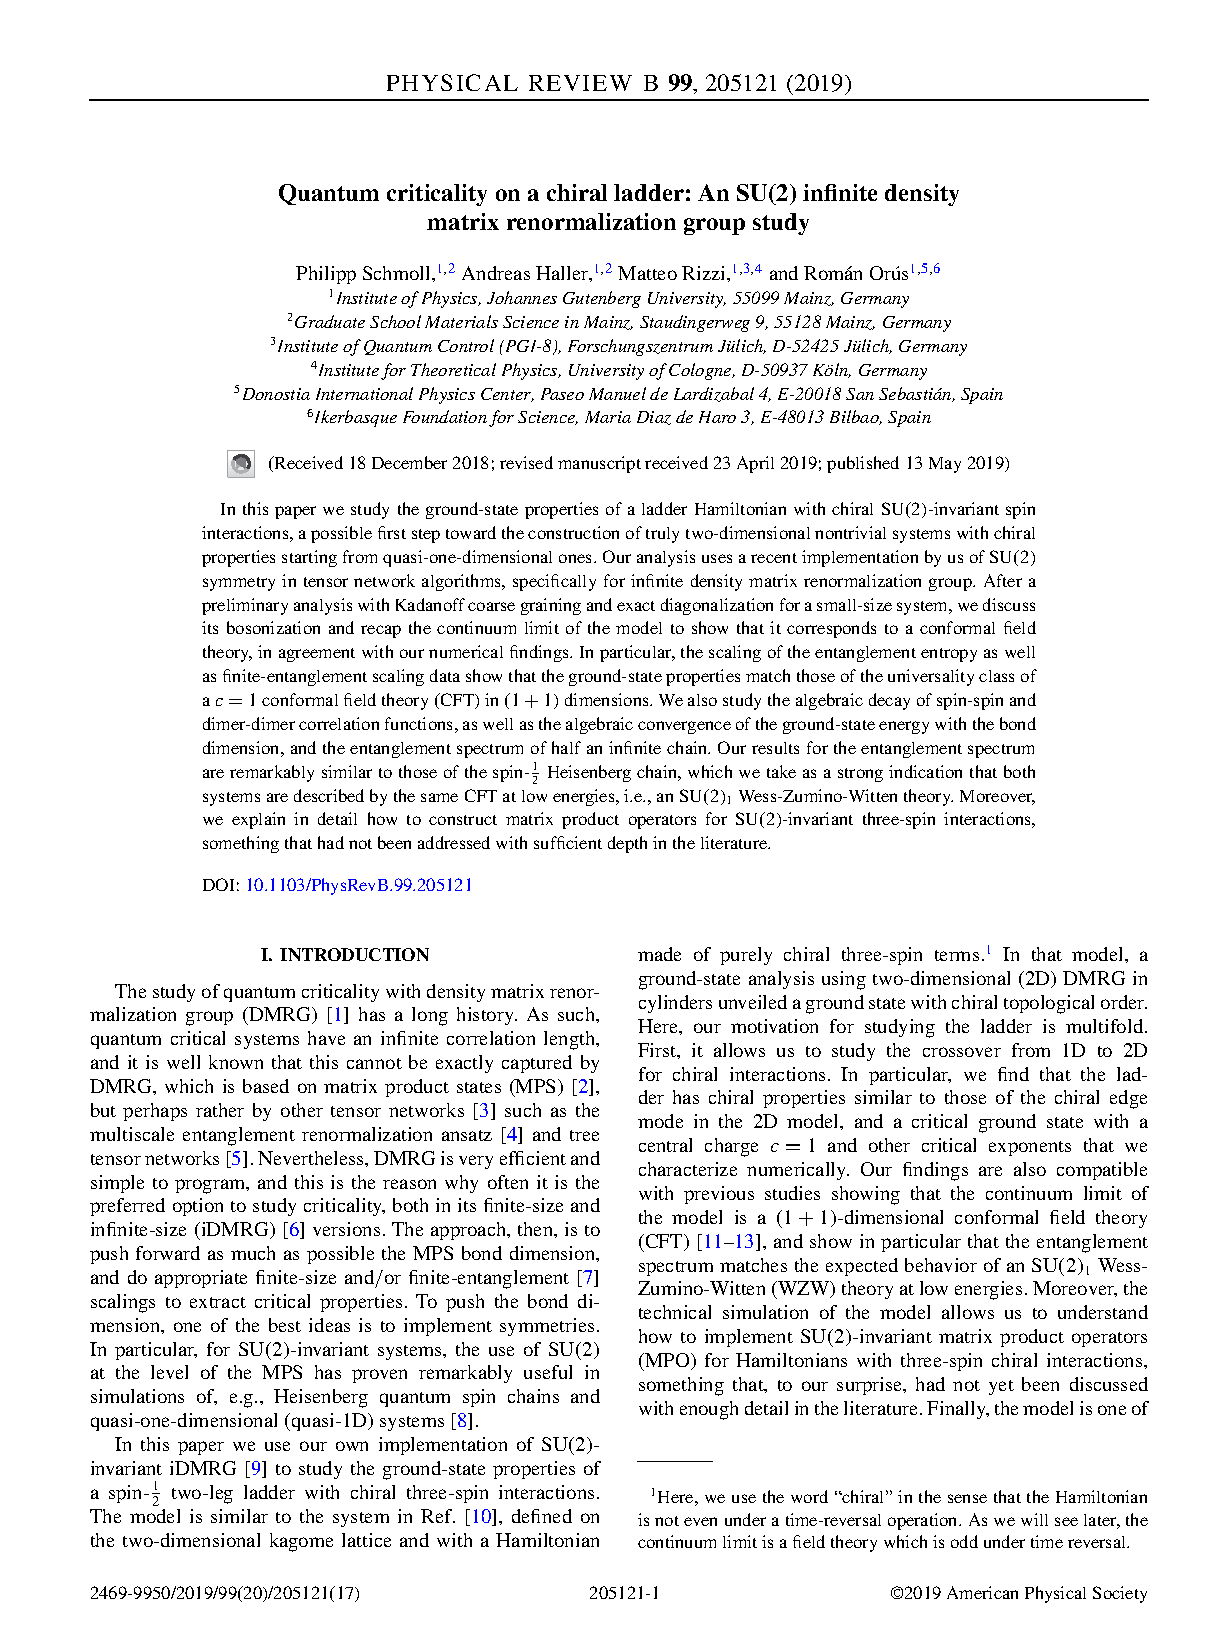
\includepdf[pages={1-}]{Library/spin_chain.pdf}
\section{The resonant state at filling factor \texorpdfstring{$\nu=1/2$}{nu=1/2} in chiral fermionic ladders}
Write intro
\includepdf[pages={2-}]{Library/pretopological_states_fermions.pdf}
\section{Exploring pretopological phases of matter in coupled wires of bosons}
Write intro
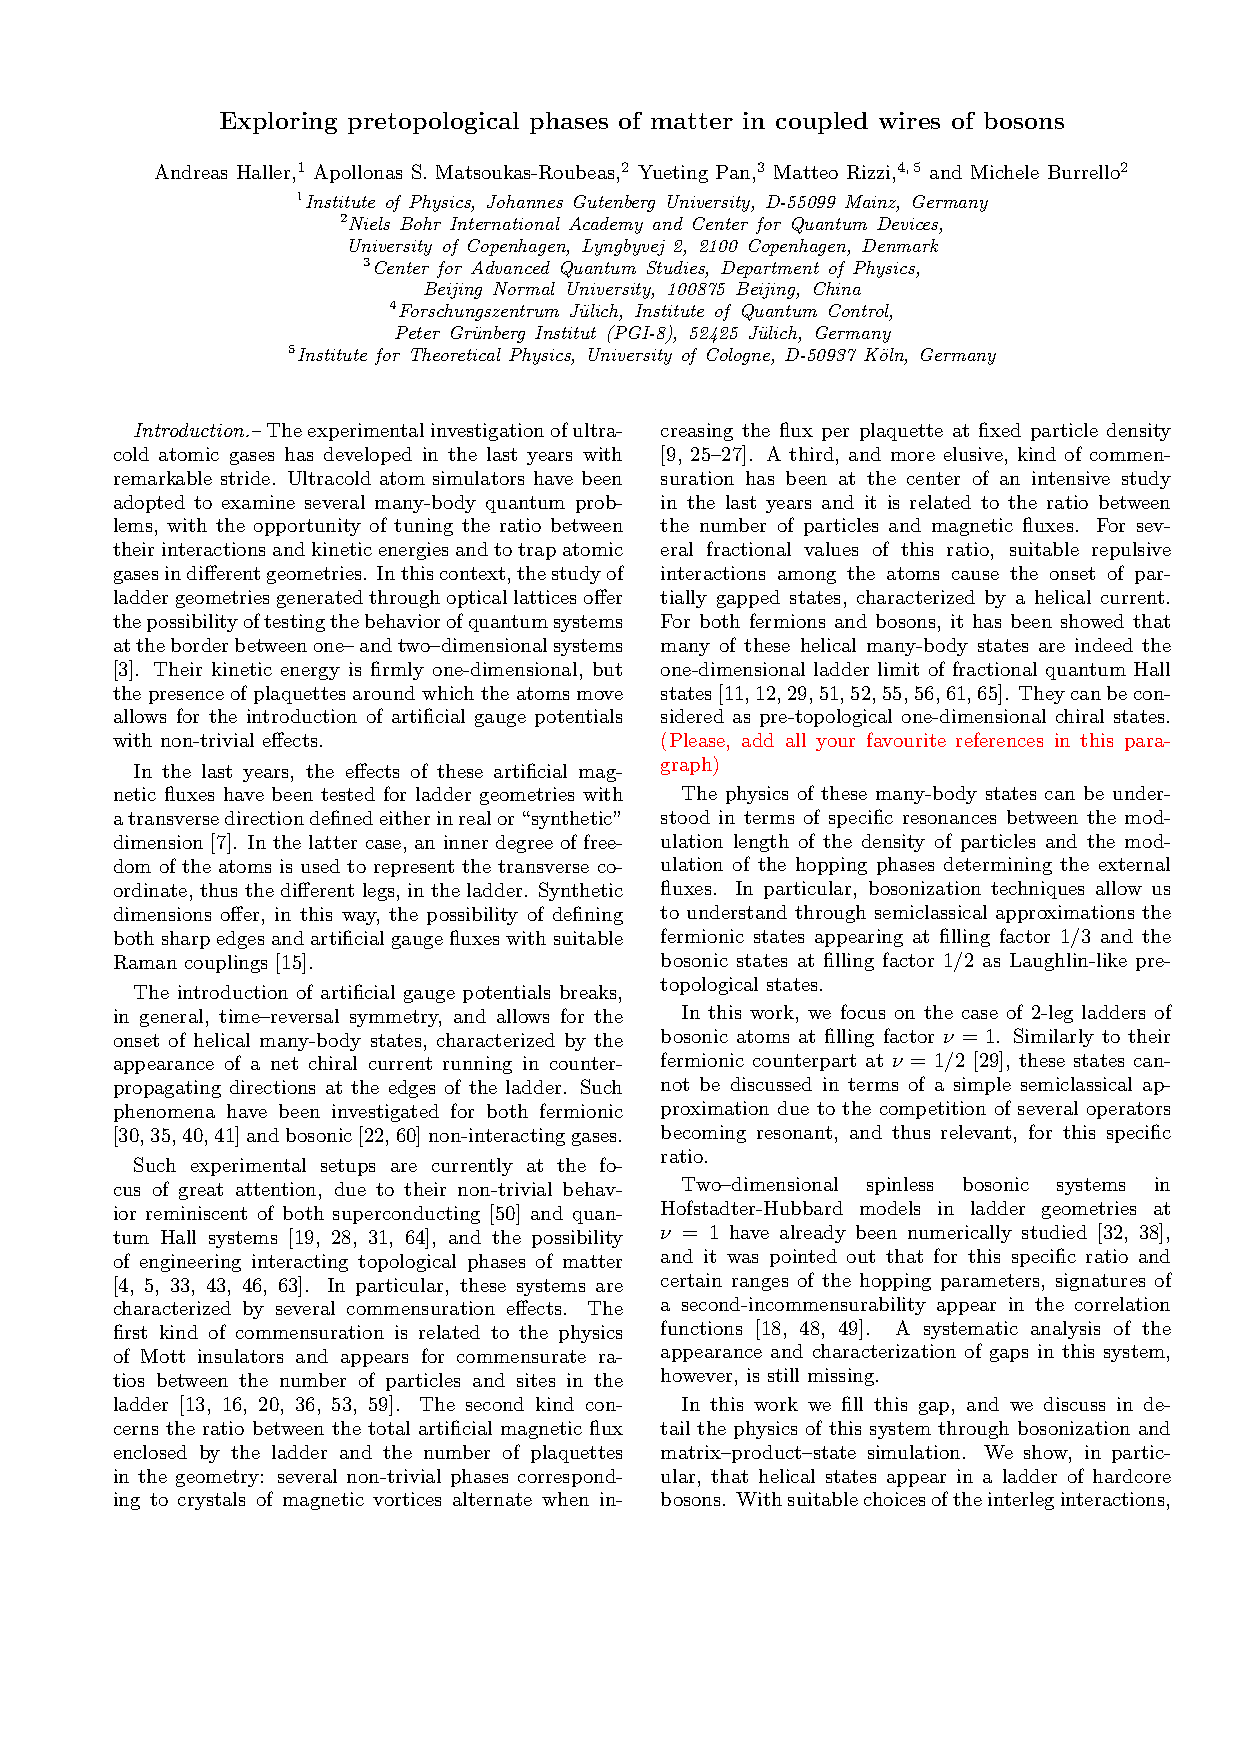
\includepdf[pages={1-}]{Library/pretopological_states_bosons.pdf}

\chapter{Tuning particle transport through interactions}
\label{ch:Tuning_particle_transport_through_interactions}
Write intro
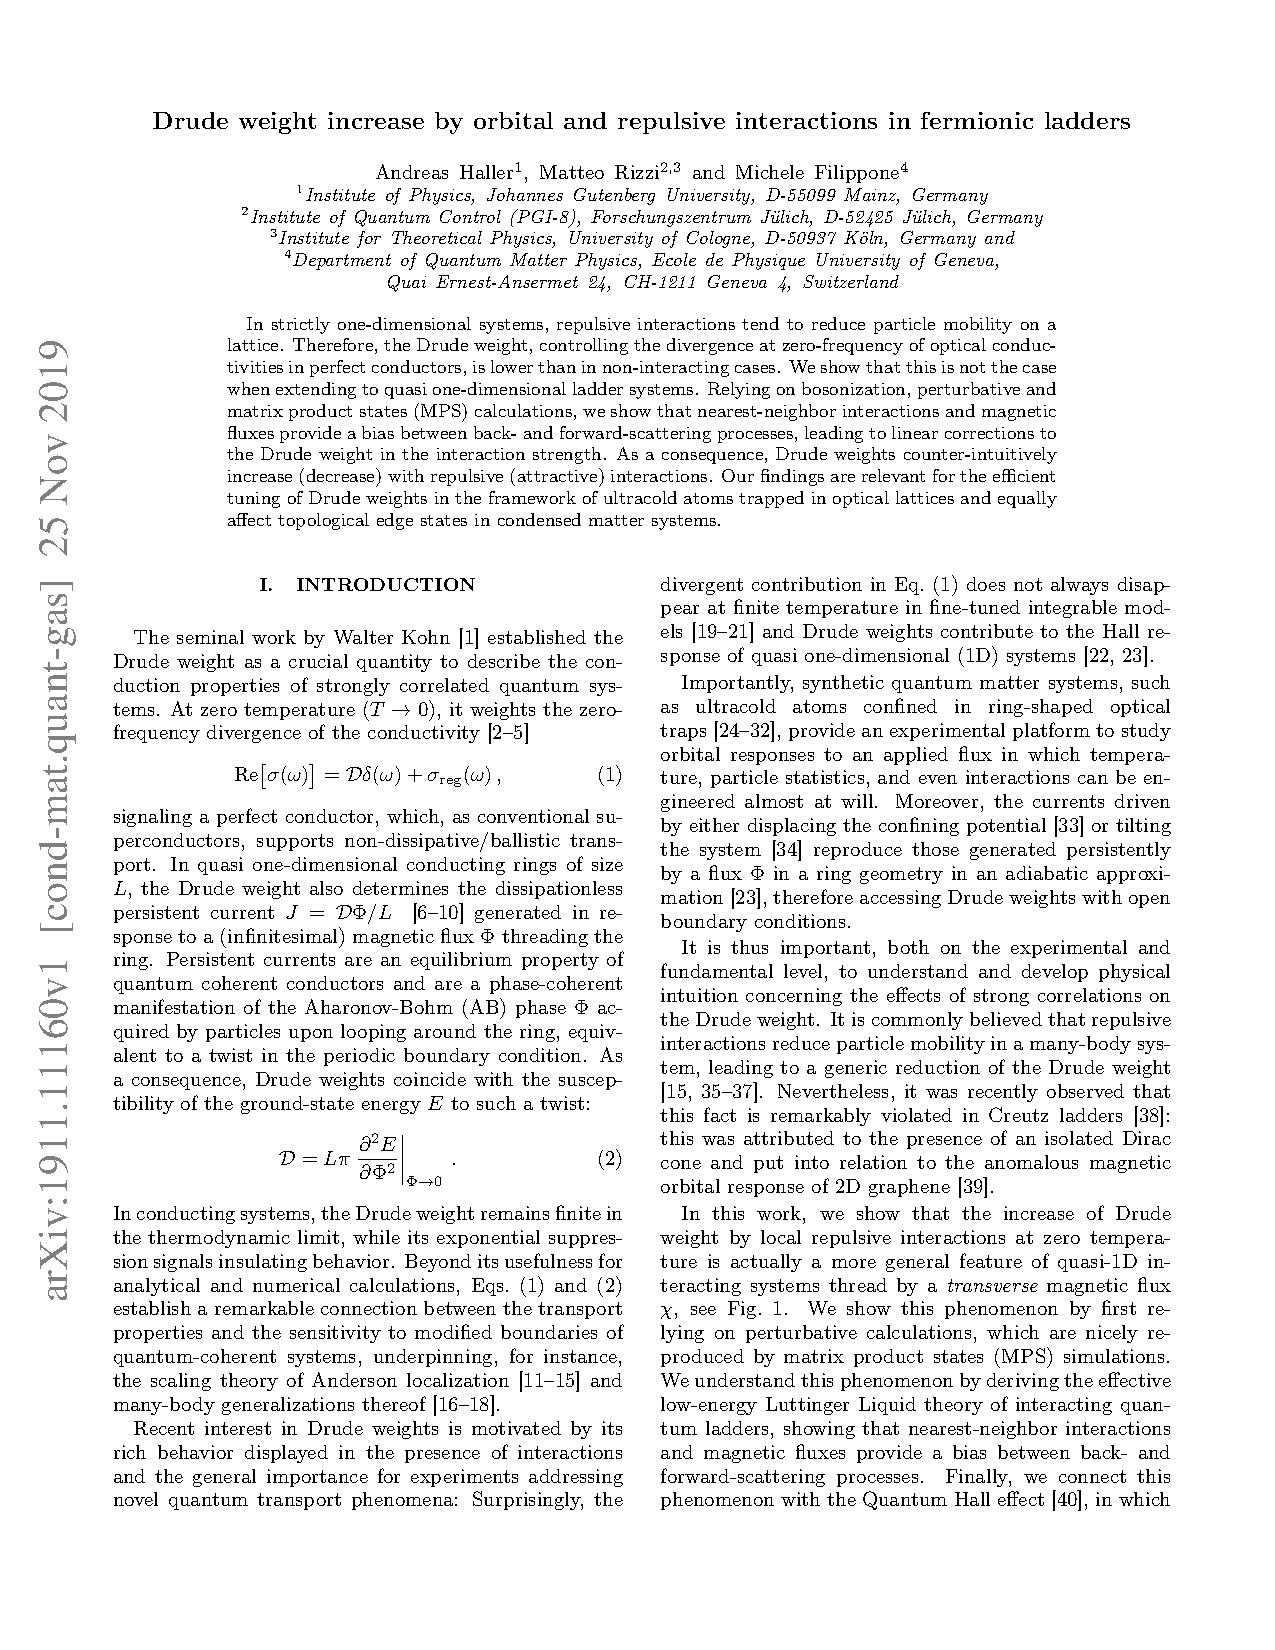
\includepdf[pages={1-}]{Library/drude_increased.pdf}


\chapter{The detection of topological invariants in real space}
\label{ch:The_detection_of_topological_invariants_in_real_space}
Write intro
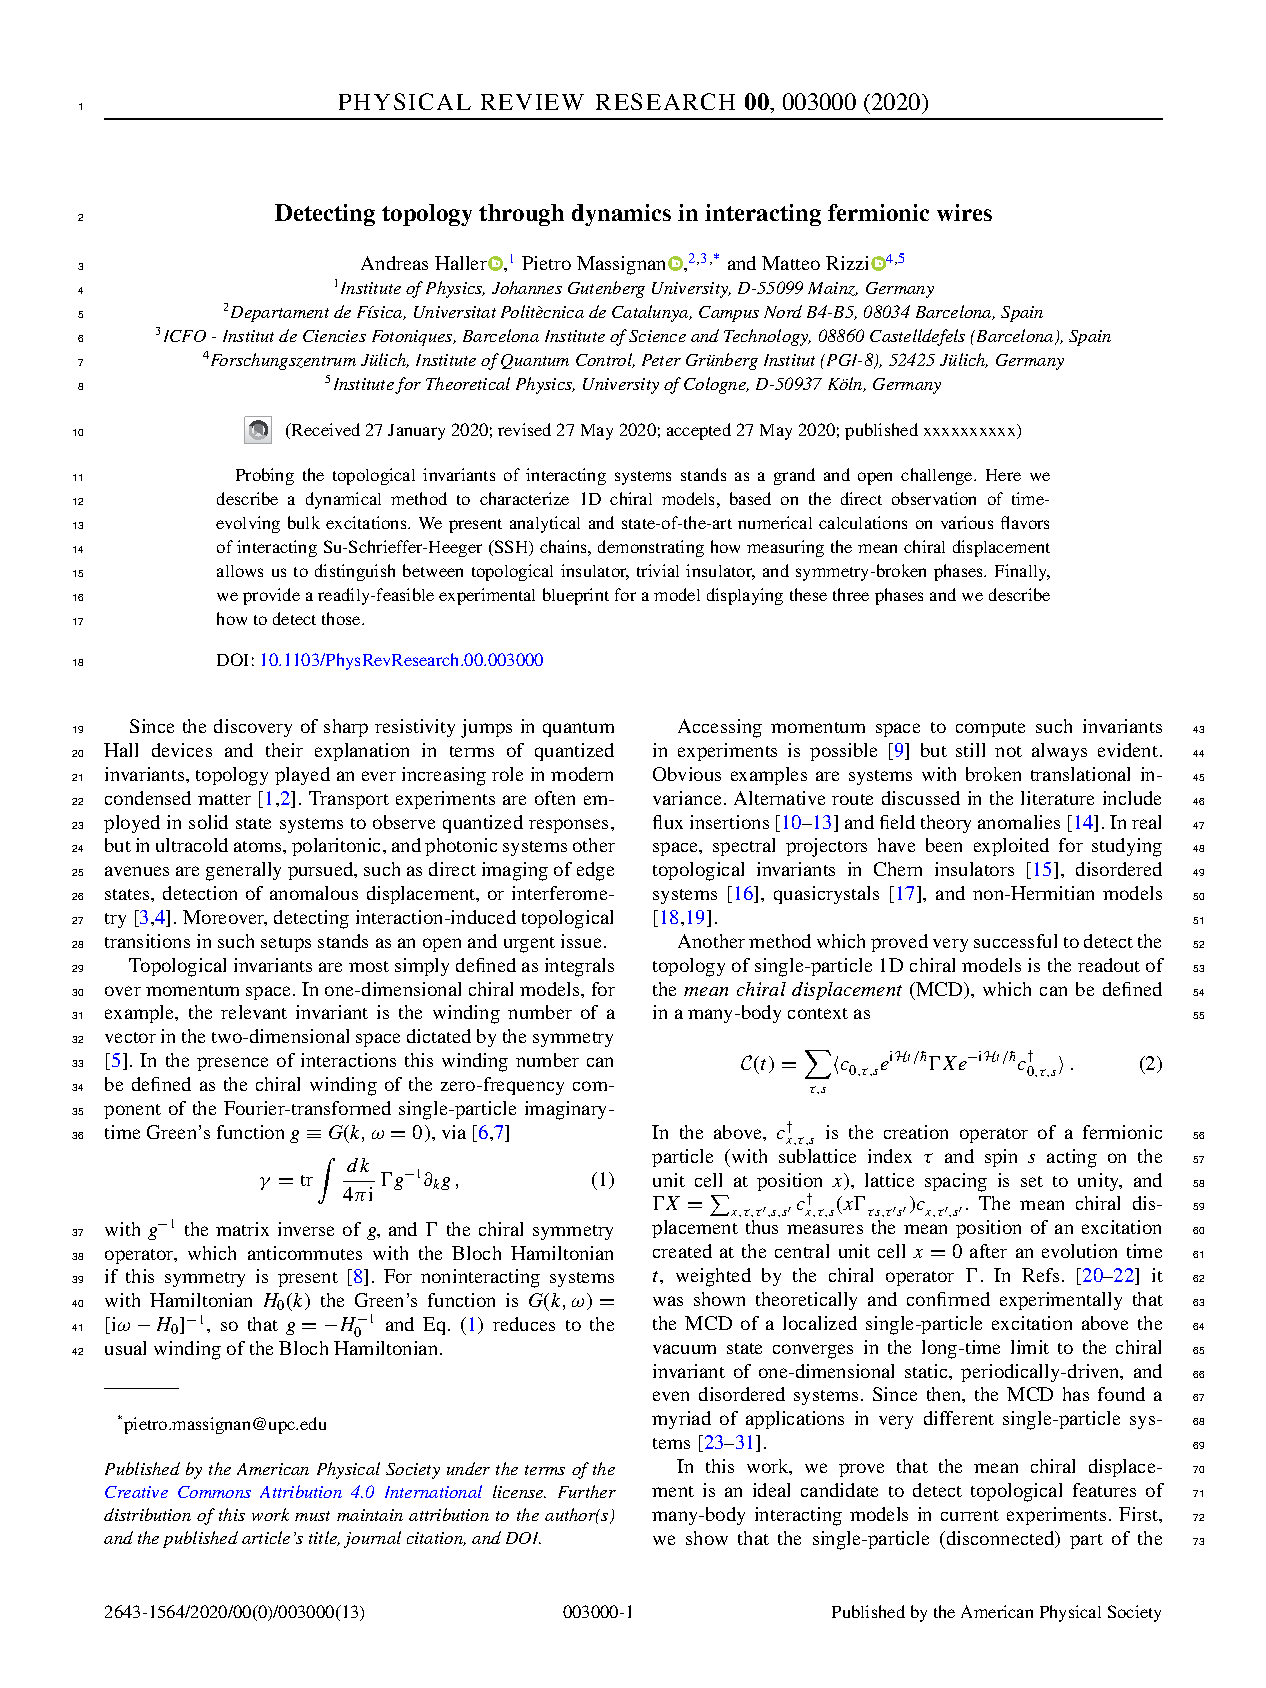
\includepdf[pages={1-}]{Library/mcd.pdf}


%%%%%%%%%%%%%%%%%%%%%%%
%!TEX root = thesis.tex
%%%%%%%%%%%%%%%%%%%%%%%
\begin{partbacktext}
    \part{Summary}
\end{partbacktext}

\include{chapter_conclusions}

%!TEX root = thesis.tex
%%%%%%%%%%%%%%%%%%%%%
\bibliographystyle{abbrvdin}
\bibliography{biblio}

% \biblstarthook{In view of the parallel print and (chapter-wise) online publication of your book at \url{www.springerlink.com} it has been decided that -- as a genreral rule --  references should be sorted chapter-wise and placed at the end of the individual chapters. However, upon agreement with your contact at Springer you may list your references in a single seperate chapter at the end of your book. Deactivate the class option \texttt{sectrefs} and the \texttt{thebibliography} environment will be put out as a chapter of its own.\\\indent
% References may be \textit{cited} in the text either by number (preferred) or by author/year.\footnote{Make sure that all references from the list are cited in the text. Those not cited should be moved to a separate \textit{Further Reading} section or chapter.} If the citatiion in the text is numbered, the reference list should be arranged in ascending order. If the citation in the text is author/year, the reference list should be \textit{sorted} alphabetically and if there are several works by the same author, the following order should be used:
% \begin{enumerate}
% \item all works by the author alone, ordered chronologically by year of publication
% \item all works by the author with a coauthor, ordered alphabetically by coauthor
% \item all works by the author with several coauthors, ordered chronologically by year of publication.
% \end{enumerate}
% The \textit{styling} of references\footnote{Always use the standard abbreviation of a journal's name according to the ISSN \textit{List of Title Word Abbreviations}, see \url{http://www.issn.org/en/node/344}} depends on the subject of your book:
% \begin{itemize}
% \item The \textit{two} recommended styles for references in books on \textit{mathematical, physical, statistical and computer sciences} are depicted in ~\cite{science-contrib, science-online, science-mono, science-journal, science-DOI} and ~\cite{phys-online, phys-mono, phys-journal, phys-DOI, phys-contrib}.
% \item Examples of the most commonly used reference style in books on \textit{Psychology, Social Sciences} are~\cite{psysoc-mono, psysoc-online,psysoc-journal, psysoc-contrib, psysoc-DOI}.
% \item Examples for references in books on \textit{Humanities, Linguistics, Philosophy} are~\cite{humlinphil-journal, humlinphil-contrib, humlinphil-mono, humlinphil-online, humlinphil-DOI}.
% \item Examples of the basic Springer style used in publications on a wide range of subjects such as \textit{Computer Science, Economics, Engineering, Geosciences, Life Sciences, Medicine, Biomedicine} are ~\cite{basic-contrib, basic-online, basic-journal, basic-DOI, basic-mono}.
% \end{itemize}
% }
% %
% \begin{thebibliography}{99.}%
% % and use \bibitem to create references.
% %
% % Use the following syntax and markup for your references if
% % the subject of your book is from the field
% % "Mathematics, Physics, Statistics, Computer Science"
% %
% % Contribution
% \bibitem{science-contrib} Broy, M.: Software engineering --- from auxiliary to key technologies. In: Broy, M., Dener, E. (eds.) Software Pioneers, pp. 10-13. Springer, Heidelberg (2002)
% %
% % Online Document
% \bibitem{science-online} Dod, J.: Effective substances. In: The Dictionary of Substances and Their Effects. Royal Society of Chemistry (1999) Available via DIALOG. \\
% \url{http://www.rsc.org/dose/title of subordinate document. Cited 15 Jan 1999}
% %
% % Monograph
% \bibitem{science-mono} Geddes, K.O., Czapor, S.R., Labahn, G.: Algorithms for Computer Algebra. Kluwer, Boston (1992)
% %
% % Journal article
% \bibitem{science-journal} Hamburger, C.: Quasimonotonicity, regularity and duality for nonlinear systems of partial differential equations. Ann. Mat. Pura. Appl. \textbf{169}, 321--354 (1995)
% %
% % Journal article by DOI
% \bibitem{science-DOI} Slifka, M.K., Whitton, J.L.: Clinical implications of dysregulated cytokine production. J. Mol. Med. (2000) doi: 10.1007/s001090000086
% %
% \bigskip
%
% % Use the following (APS) syntax and markup for your references if
% % the subject of your book is from the field
% % "Mathematics, Physics, Statistics, Computer Science"
% %
% % Online Document
% \bibitem{phys-online} J. Dod, in \textit{The Dictionary of Substances and Their Effects}, Royal Society of Chemistry. (Available via DIALOG, 1999),
% \url{http://www.rsc.org/dose/title of subordinate document. Cited 15 Jan 1999}
% %
% % Monograph
% \bibitem{phys-mono} H. Ibach, H. L\"uth, \textit{Solid-State Physics}, 2nd edn. (Springer, New York, 1996), pp. 45-56
% %
% % Journal article
% \bibitem{phys-journal} S. Preuss, A. Demchuk Jr., M. Stuke, Appl. Phys. A \textbf{61}
% %
% % Journal article by DOI
% \bibitem{phys-DOI} M.K. Slifka, J.L. Whitton, J. Mol. Med., doi: 10.1007/s001090000086
% %
% % Contribution
% \bibitem{phys-contrib} S.E. Smith, in \textit{Neuromuscular Junction}, ed. by E. Zaimis. Handbook of Experimental Pharmacology, vol 42 (Springer, Heidelberg, 1976), p. 593
% %
% \bigskip
% %
% % Use the following syntax and markup for your references if
% % the subject of your book is from the field
% % "Psychology, Social Sciences"
% %
% %
% % Monograph
% \bibitem{psysoc-mono} Calfee, R.~C., \& Valencia, R.~R. (1991). \textit{APA guide to preparing manuscripts for journal publication.} Washington, DC: American Psychological Association.
% %
% % Online Document
% \bibitem{psysoc-online} Dod, J. (1999). Effective substances. In: The dictionary of substances and their effects. Royal Society of Chemistry. Available via DIALOG. \\
% \url{http://www.rsc.org/dose/Effective substances.} Cited 15 Jan 1999.
% %
% % Journal article
% \bibitem{psysoc-journal} Harris, M., Karper, E., Stacks, G., Hoffman, D., DeNiro, R., Cruz, P., et al. (2001). Writing labs and the Hollywood connection. \textit{J Film} Writing, 44(3), 213--245.
% %
% % Contribution
% \bibitem{psysoc-contrib} O'Neil, J.~M., \& Egan, J. (1992). Men's and women's gender role journeys: Metaphor for healing, transition, and transformation. In B.~R. Wainrig (Ed.), \textit{Gender issues across the life cycle} (pp. 107--123). New York: Springer.
% %
% % Journal article by DOI
% \bibitem{psysoc-DOI}Kreger, M., Brindis, C.D., Manuel, D.M., Sassoubre, L. (2007). Lessons learned in systems change initiatives: benchmarks and indicators. \textit{American Journal of Community Psychology}, doi: 10.1007/s10464-007-9108-14.
% %
% %
% % Use the following syntax and markup for your references if
% % the subject of your book is from the field
% % "Humanities, Linguistics, Philosophy"
% %
% \bigskip
% %
% % Journal article
% \bibitem{humlinphil-journal} Alber John, Daniel C. O'Connell, and Sabine Kowal. 2002. Personal perspective in TV interviews. \textit{Pragmatics} 12:257--271
% %
% % Contribution
% \bibitem{humlinphil-contrib} Cameron, Deborah. 1997. Theoretical debates in feminist linguistics: Questions of sex and gender. In \textit{Gender and discourse}, ed. Ruth Wodak, 99--119. London: Sage Publications.
% %
% % Monograph
% \bibitem{humlinphil-mono} Cameron, Deborah. 1985. \textit{Feminism and linguistic theory.} New York: St. Martin's Press.
% %
% % Online Document
% \bibitem{humlinphil-online} Dod, Jake. 1999. Effective substances. In: The dictionary of substances and their effects. Royal Society of Chemistry. Available via DIALOG. \\
% http://www.rsc.org/dose/title of subordinate document. Cited 15 Jan 1999
% %
% % Journal article by DOI
% \bibitem{humlinphil-DOI} Suleiman, Camelia, Daniel C. O'Connell, and Sabine Kowal. 2002. `If you and I, if we, in this later day, lose that sacred fire...': Perspective in political interviews. \textit{Journal of Psycholinguistic Research}. doi: 10.1023/A:1015592129296.
% %
% %
% %
% \bigskip
% %
% %
% % Use the following syntax and markup for your references if
% % the subject of your book is from the field
% % "Computer Science, Economics, Engineering, Geosciences, Life Sciences"
% %
% %
% % Contribution
% \bibitem{basic-contrib} Brown B, Aaron M (2001) The politics of nature. In: Smith J (ed) The rise of modern genomics, 3rd edn. Wiley, New York
% %
% % Online Document
% \bibitem{basic-online} Dod J (1999) Effective Substances. In: The dictionary of substances and their effects. Royal Society of Chemistry. Available via DIALOG. \\
% \url{http://www.rsc.org/dose/title of subordinate document. Cited 15 Jan 1999}
% %
% % Journal article by DOI
% \bibitem{basic-DOI} Slifka MK, Whitton JL (2000) Clinical implications of dysregulated cytokine production. J Mol Med, doi: 10.1007/s001090000086
% %
% % Journal article
% \bibitem{basic-journal} Smith J, Jones M Jr, Houghton L et al (1999) Future of health insurance. N Engl J Med 965:325--329
% %
% % Monograph
% \bibitem{basic-mono} South J, Blass B (2001) The future of modern genomics. Blackwell, London
% %
% \end{thebibliography}


%!TEX root = thesis.tex
%%%%%%%%%%%%%%%%%%%%%
\appendix
\motto{All's well that ends well}
% \chapter{Chapter Heading}
% \label{introA} % Always give a unique label
% % use \chaptermark{}
% % to alter or adjust the chapter heading in the running head
%
% Use the template \emph{appendix.tex} together with the Springer document class SVMono (monograph-type books) or SVMult (edited books) to style appendix of your book.
%
%
% \section{Section Heading}
% \label{sec:A1}
% % Always give a unique label
% % and use \ref{<label>} for cross-references
% % and \cite{<label>} for bibliographic references
% % use \sectionmark{}
% % to alter or adjust the section heading in the running head
% Instead of simply listing headings of different levels we recommend to let every heading be followed by at least a short passage of text. Furtheron please use the \LaTeX\ automatism for all your cross-references and citations.
%
%
% \subsection{Subsection Heading}
% \label{sec:A2}
% Instead of simply listing headings of different levels we recommend to let every heading be followed by at least a short passage of text. Furtheron please use the \LaTeX\ automatism for all your cross-references and citations as has already been described in Sect.~\ref{sec:A1}.
%
% For multiline equations we recommend to use the \verb|eqnarray| environment.
% \begin{eqnarray}
% \vec{a}\times\vec{b}=\vec{c} \nonumber\\
% \vec{a}\times\vec{b}=\vec{c}
% \label{eq:A01}
% \end{eqnarray}
%
% \subsubsection{Subsubsection Heading}
% Instead of simply listing headings of different levels we recommend to let every heading be followed by at least a short passage of text. Furtheron please use the \LaTeX\ automatism for all your cross-references and citations as has already been described in Sect.~\ref{sec:A2}.
%
% Please note that the first line of text that follows a heading is not indented, whereas the first lines of all subsequent paragraphs are.
%
% % For figures use
% %
% \begin{figure}[t]
% \sidecaption[t]
% %\centering
% % Use the relevant command for your figure-insertion program
% % to insert the figure file.
% % For example, with the option graphics use
% \includegraphics[scale=.65]{figure}
% %
% % If not, use
% %\picplace{5cm}{2cm} % Give the correct figure height and width in cm
% %
% \caption{Please write your figure caption here}
% \label{fig:A1}       % Give a unique label
% \end{figure}
%
% % For tables use
% %
% \begin{table}
% \caption{Please write your table caption here}
% \label{tab:A1}       % Give a unique label
% %
% % For LaTeX tables use
% %
% \begin{tabular}{p{2cm}p{2.4cm}p{2cm}p{4.9cm}}
% \hline\noalign{\smallskip}
% Classes & Subclass & Length & Action Mechanism  \\
% \noalign{\smallskip}\hline\noalign{\smallskip}
% Translation & mRNA$^a$  & 22 (19--25) & Translation repression, mRNA cleavage\\
% Translation & mRNA cleavage & 21 & mRNA cleavage\\
% Translation & mRNA  & 21--22 & mRNA cleavage\\
% Translation & mRNA  & 24--26 & Histone and DNA Modification\\
% \noalign{\smallskip}\hline\noalign{\smallskip}
% \end{tabular}
% $^a$ Table foot note (with superscript)
% \end{table}
% %


\backmatter%%%%%%%%%%%%%%%%%%%%%%%%%%%%%%%%%%%%%%%%%%%%%%%%%%%%%%%%%%%%%%%%%%%%%
% \printindex

\end{document}
